\documentclass{article}
\usepackage{amsmath}
\usepackage{listings}
\usepackage{algorithm2e}
\usepackage{enumitem}
\usepackage{graphicx}
\graphicspath{./}
\begin{document}
\title {CS 260 Homework 4}
\author{Semanti Basu}
\maketitle


\section*{Question 1}
The binary trees are:



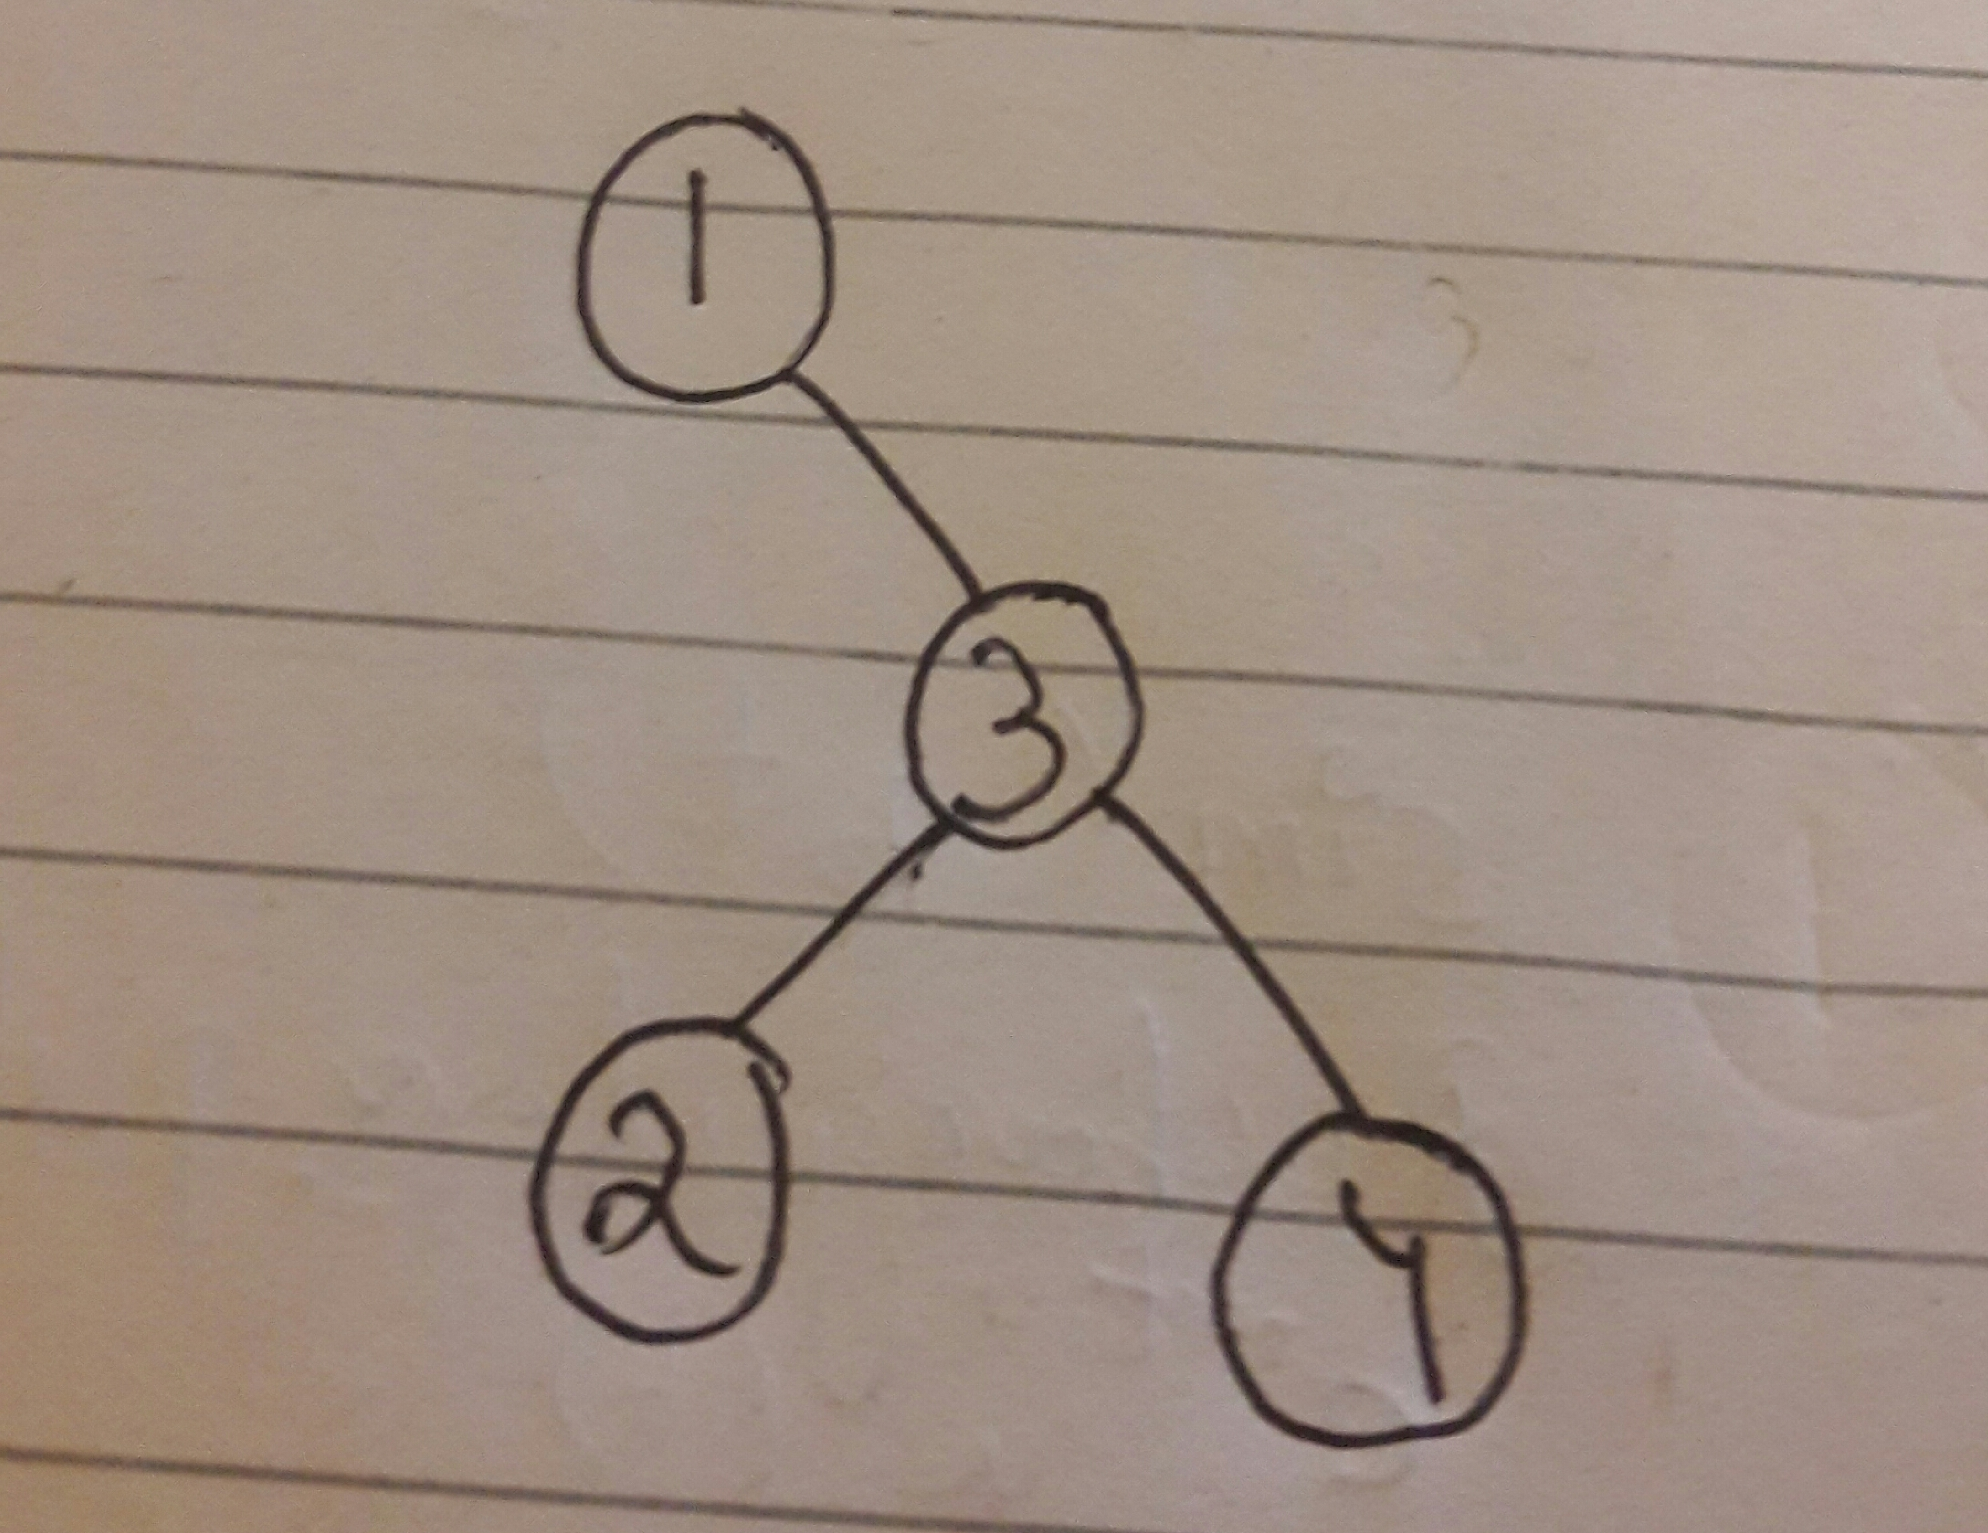
\includegraphics[scale=0.05]{1.jpg}



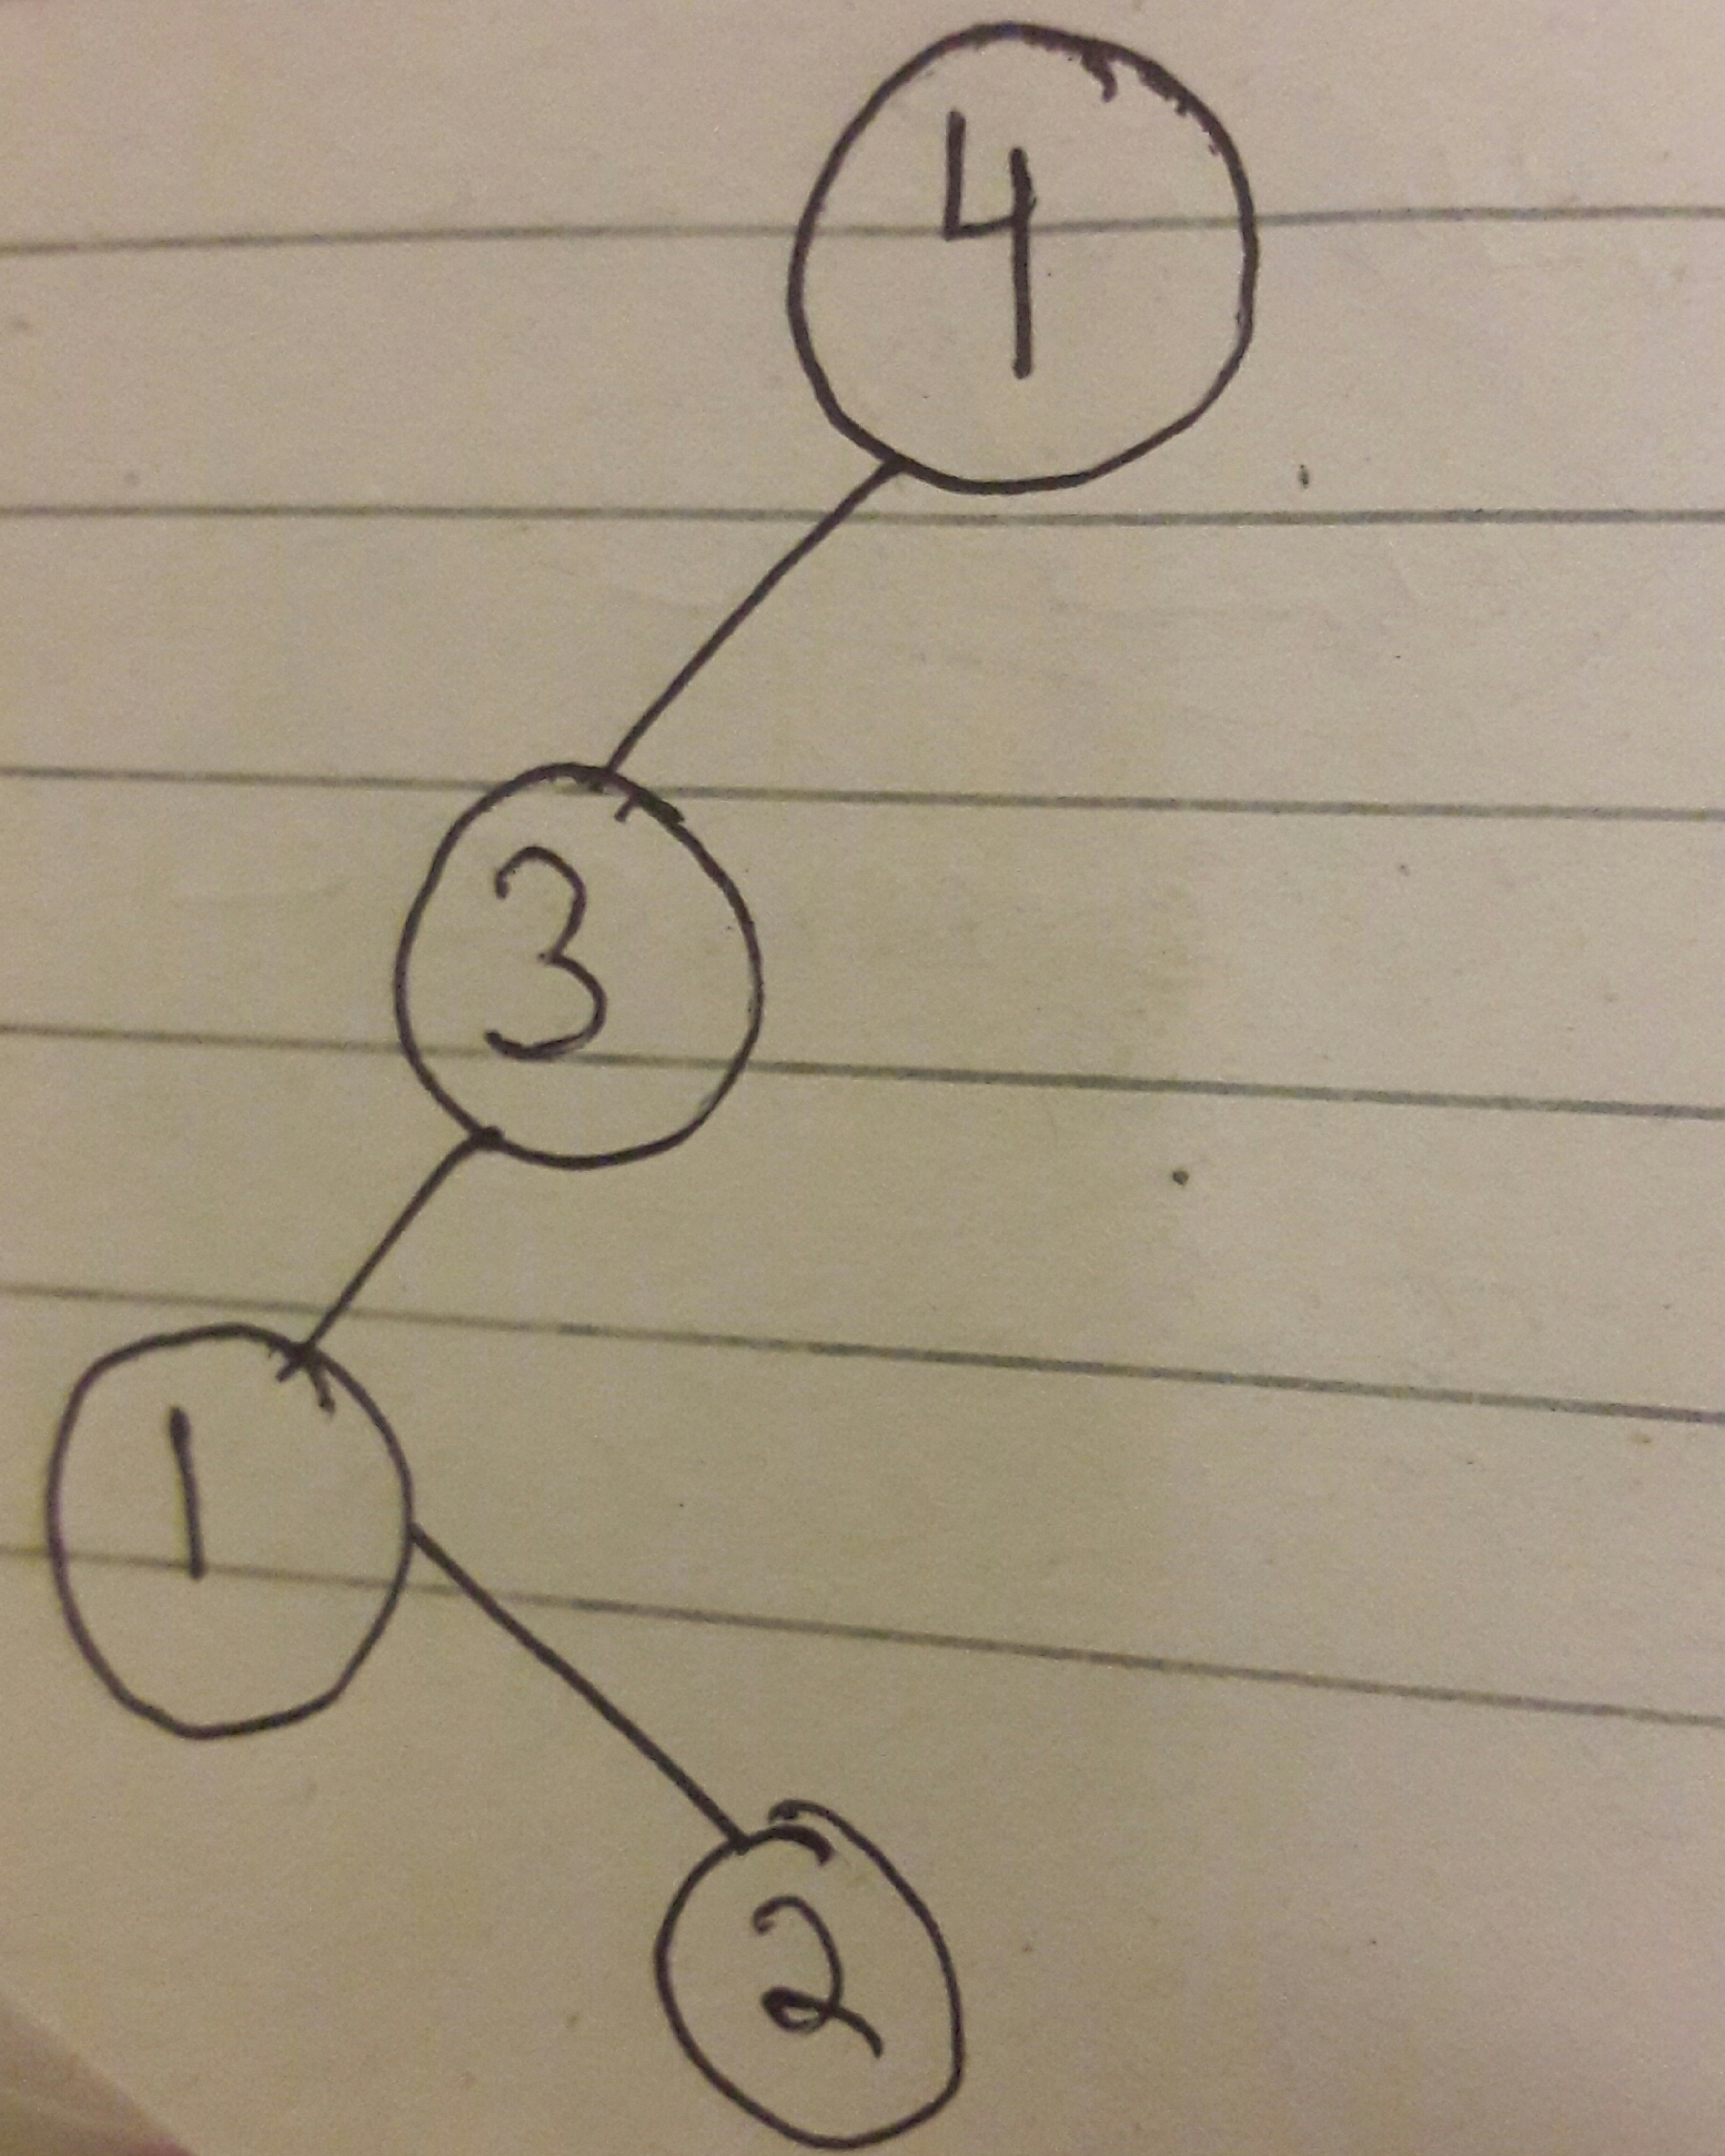
\includegraphics[scale=0.05]{2.jpg}




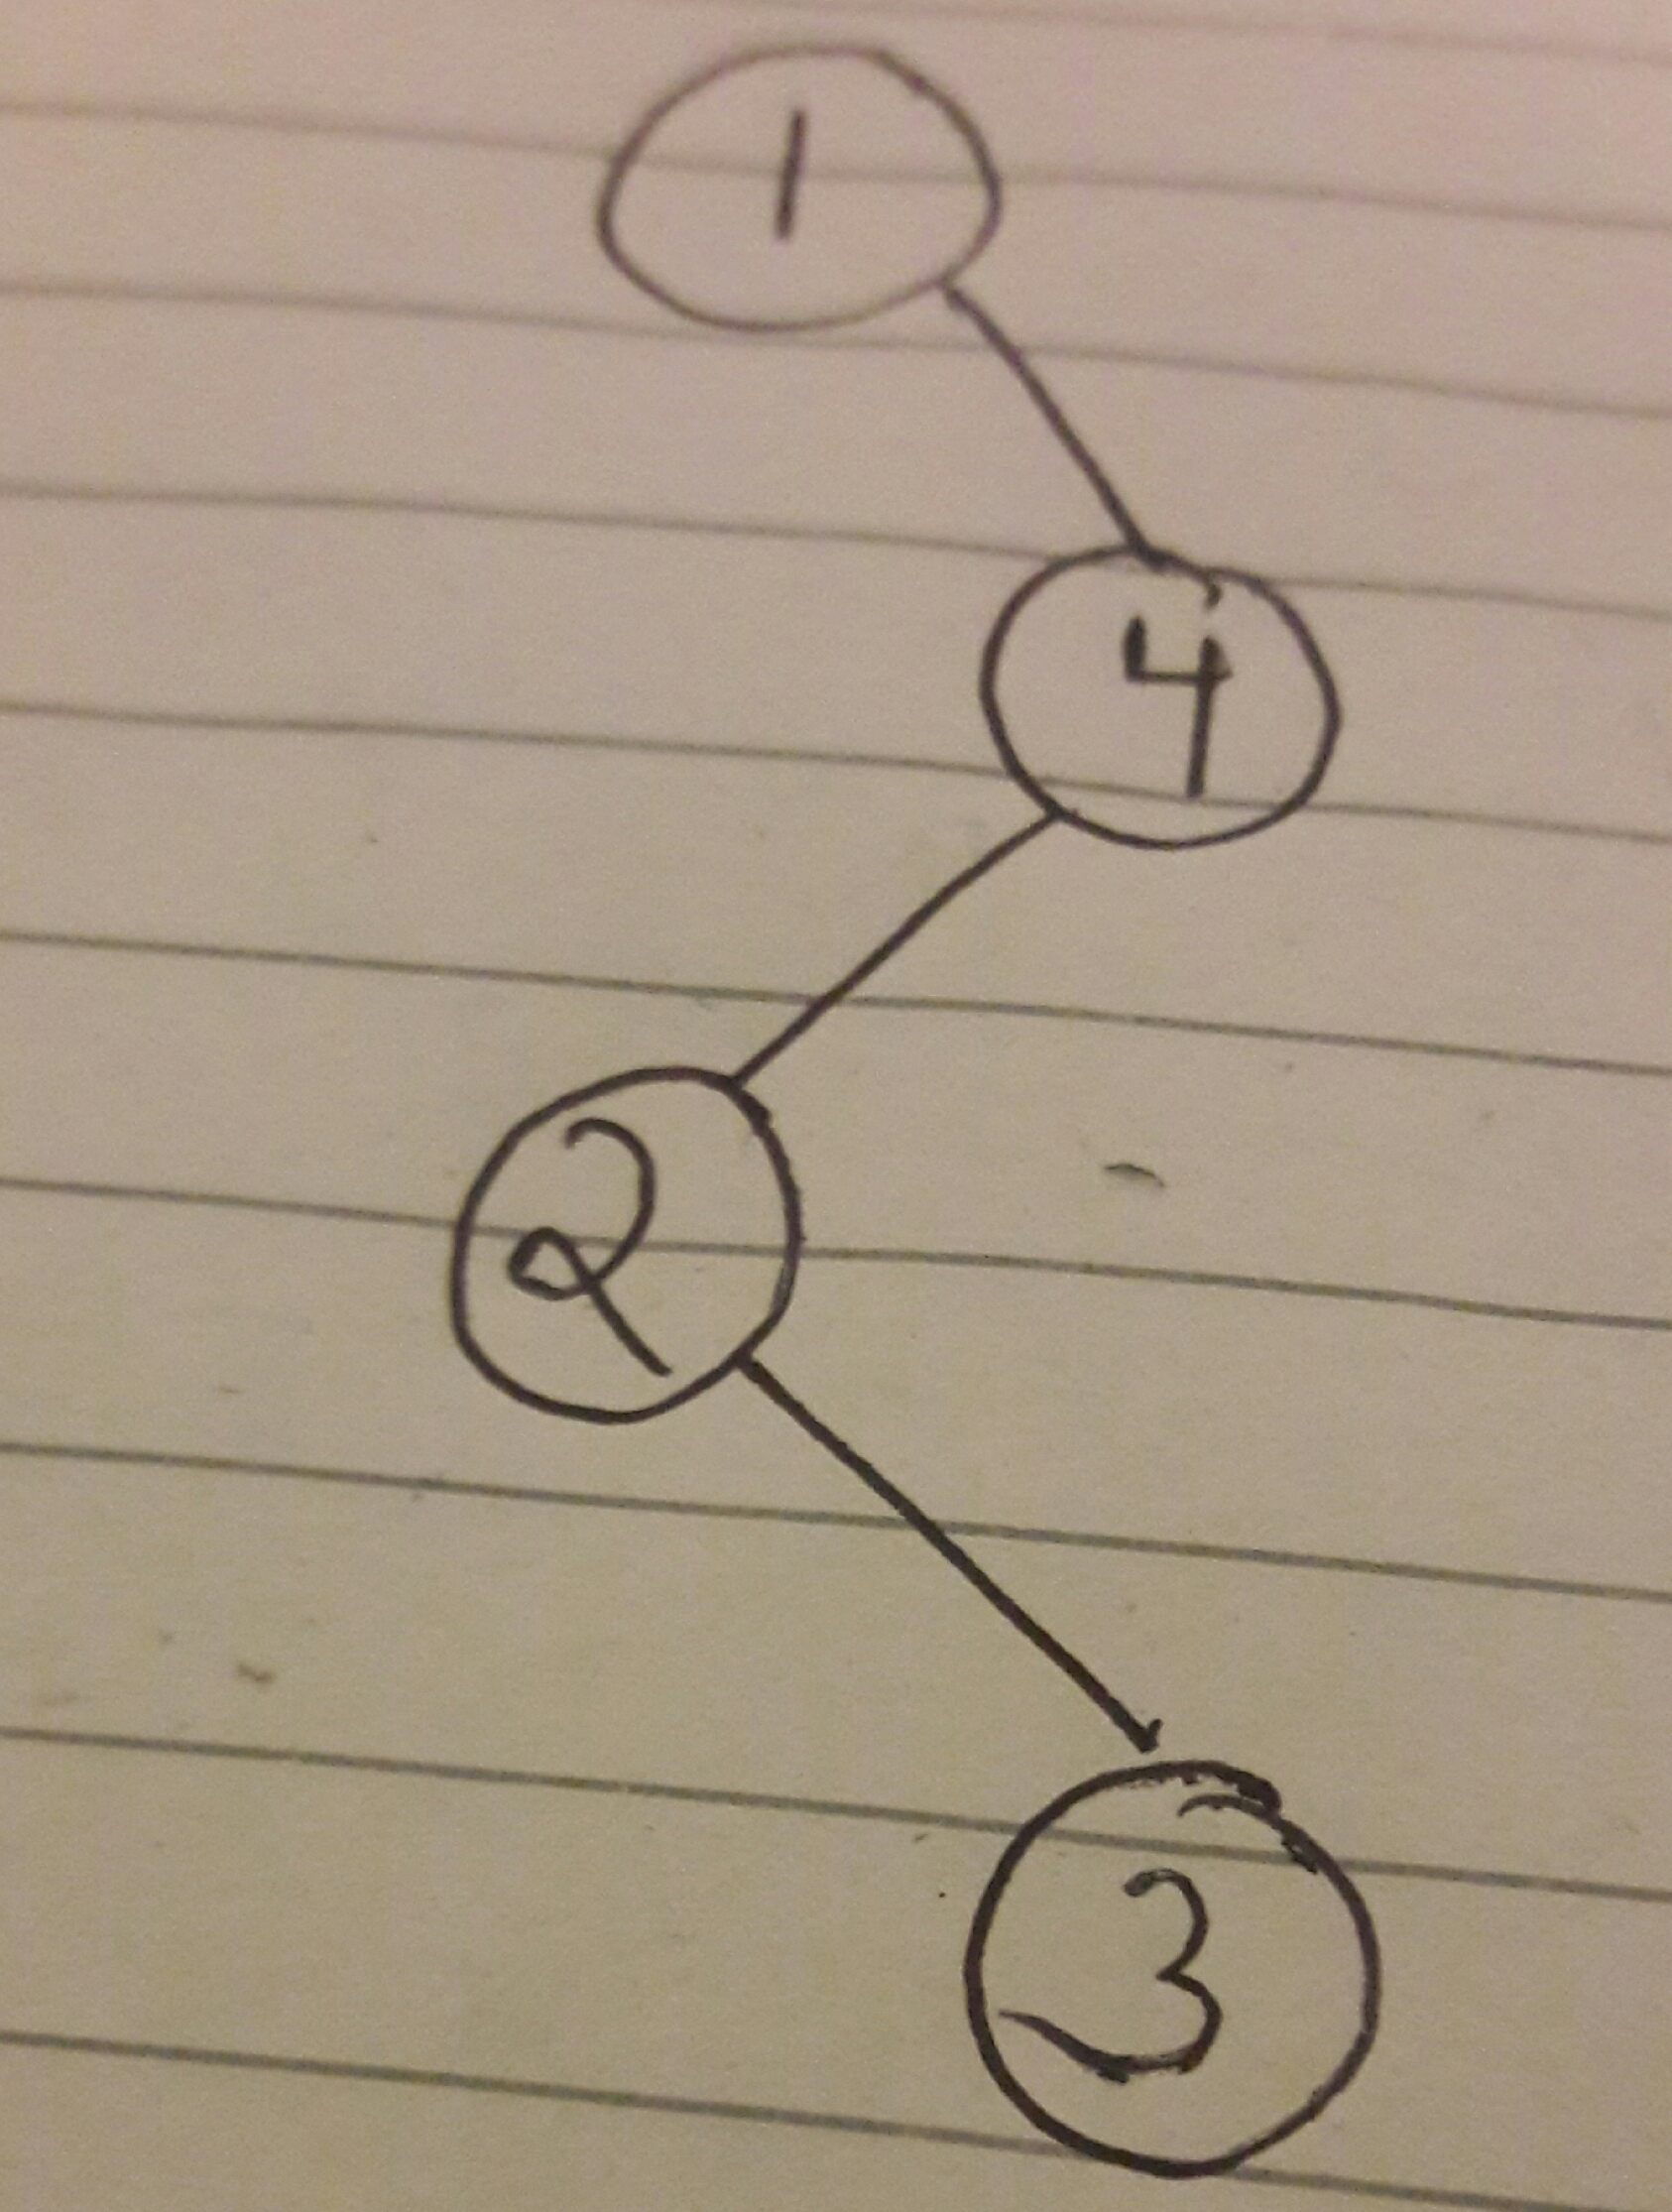
\includegraphics[scale=0.05]{3.jpg}






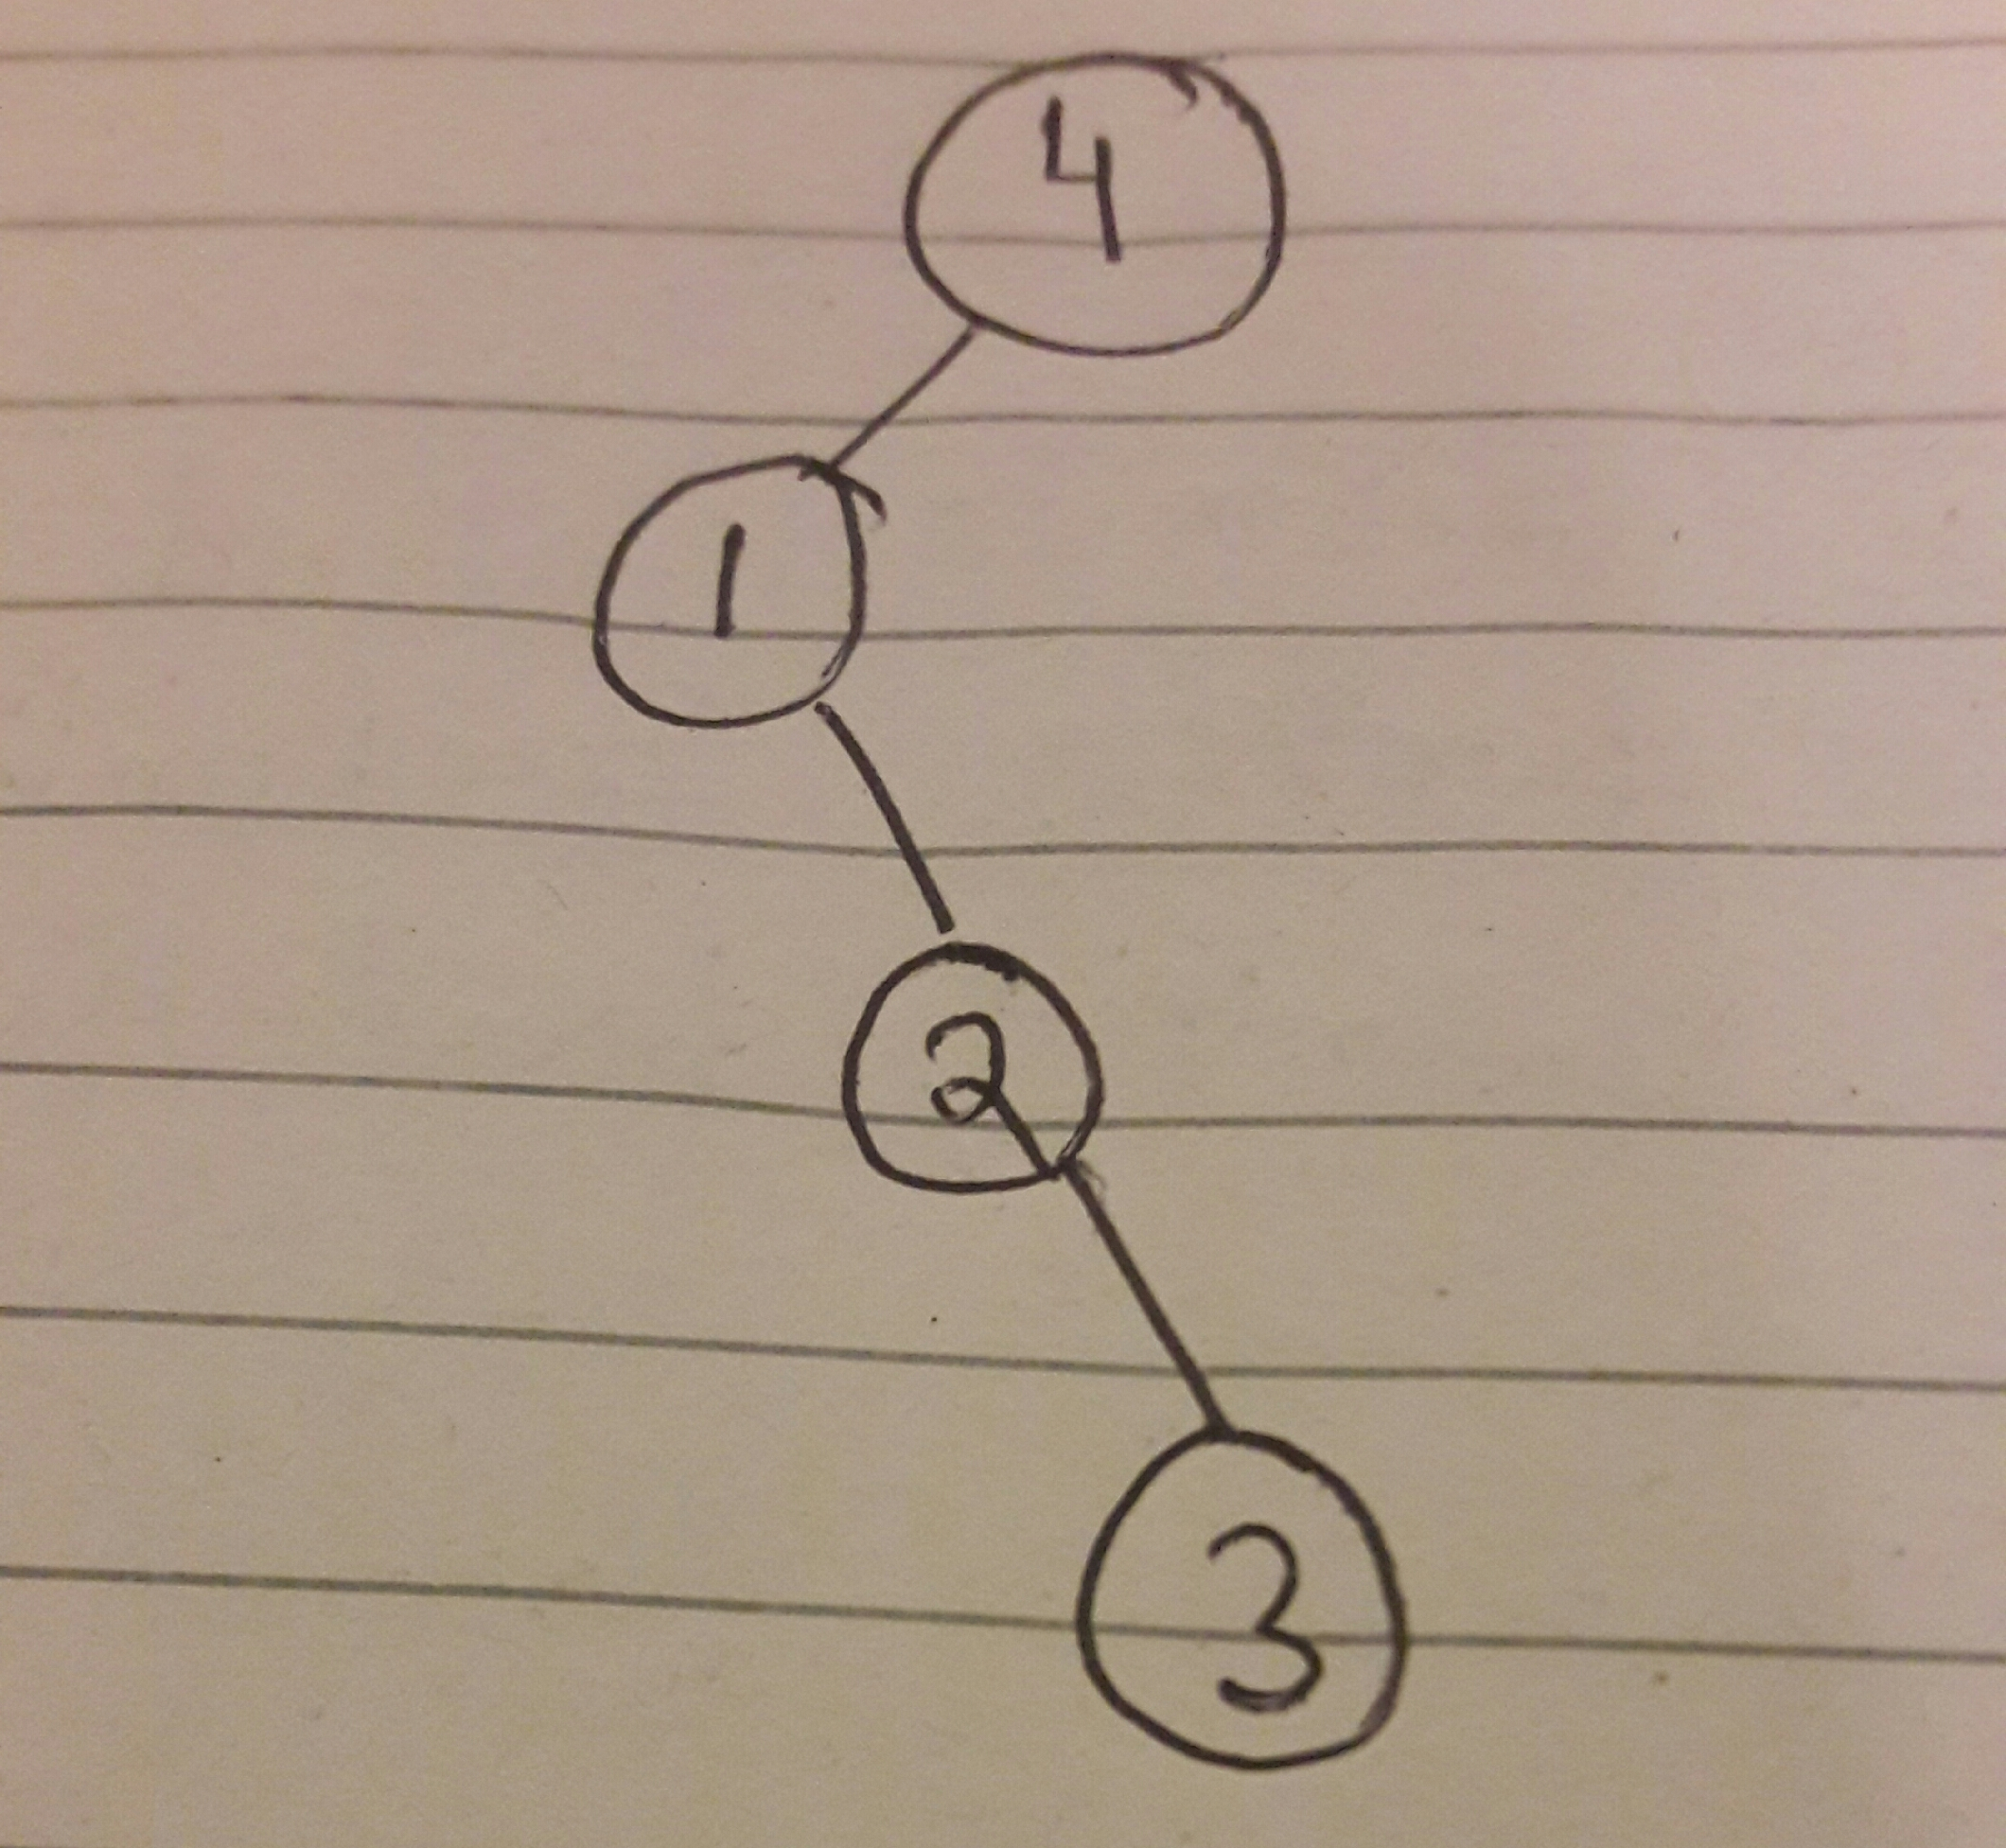
\includegraphics[scale=0.05]{4.jpg}






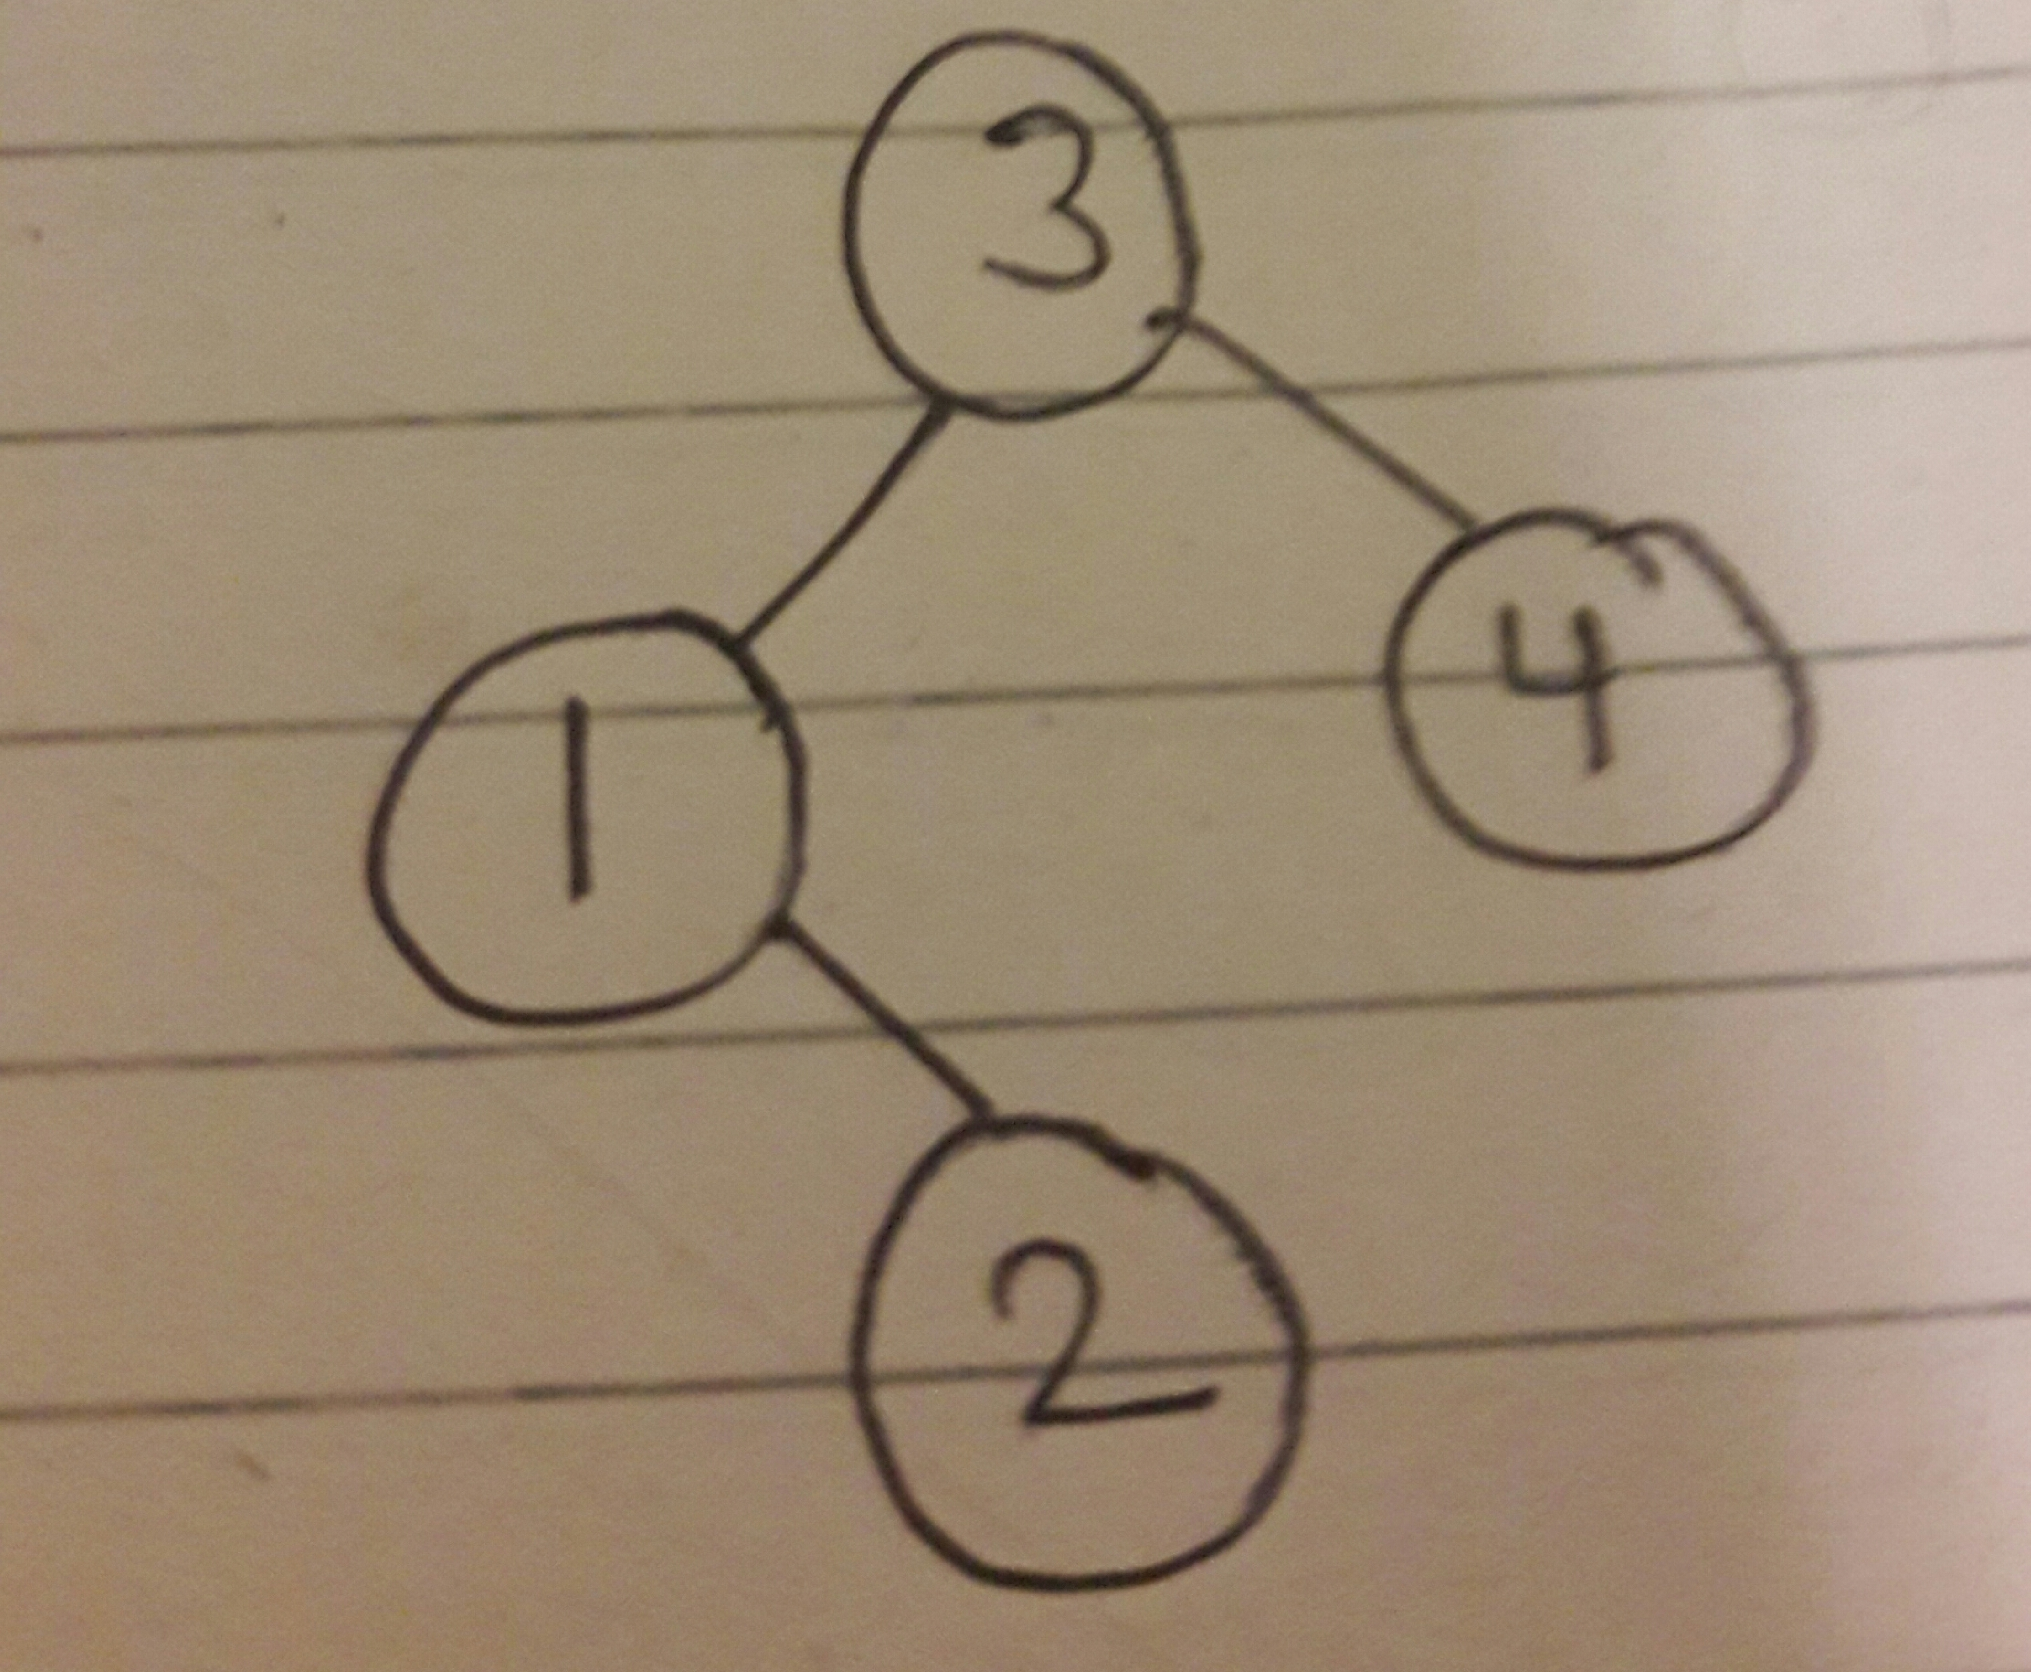
\includegraphics[scale=0.05]{5.jpg}




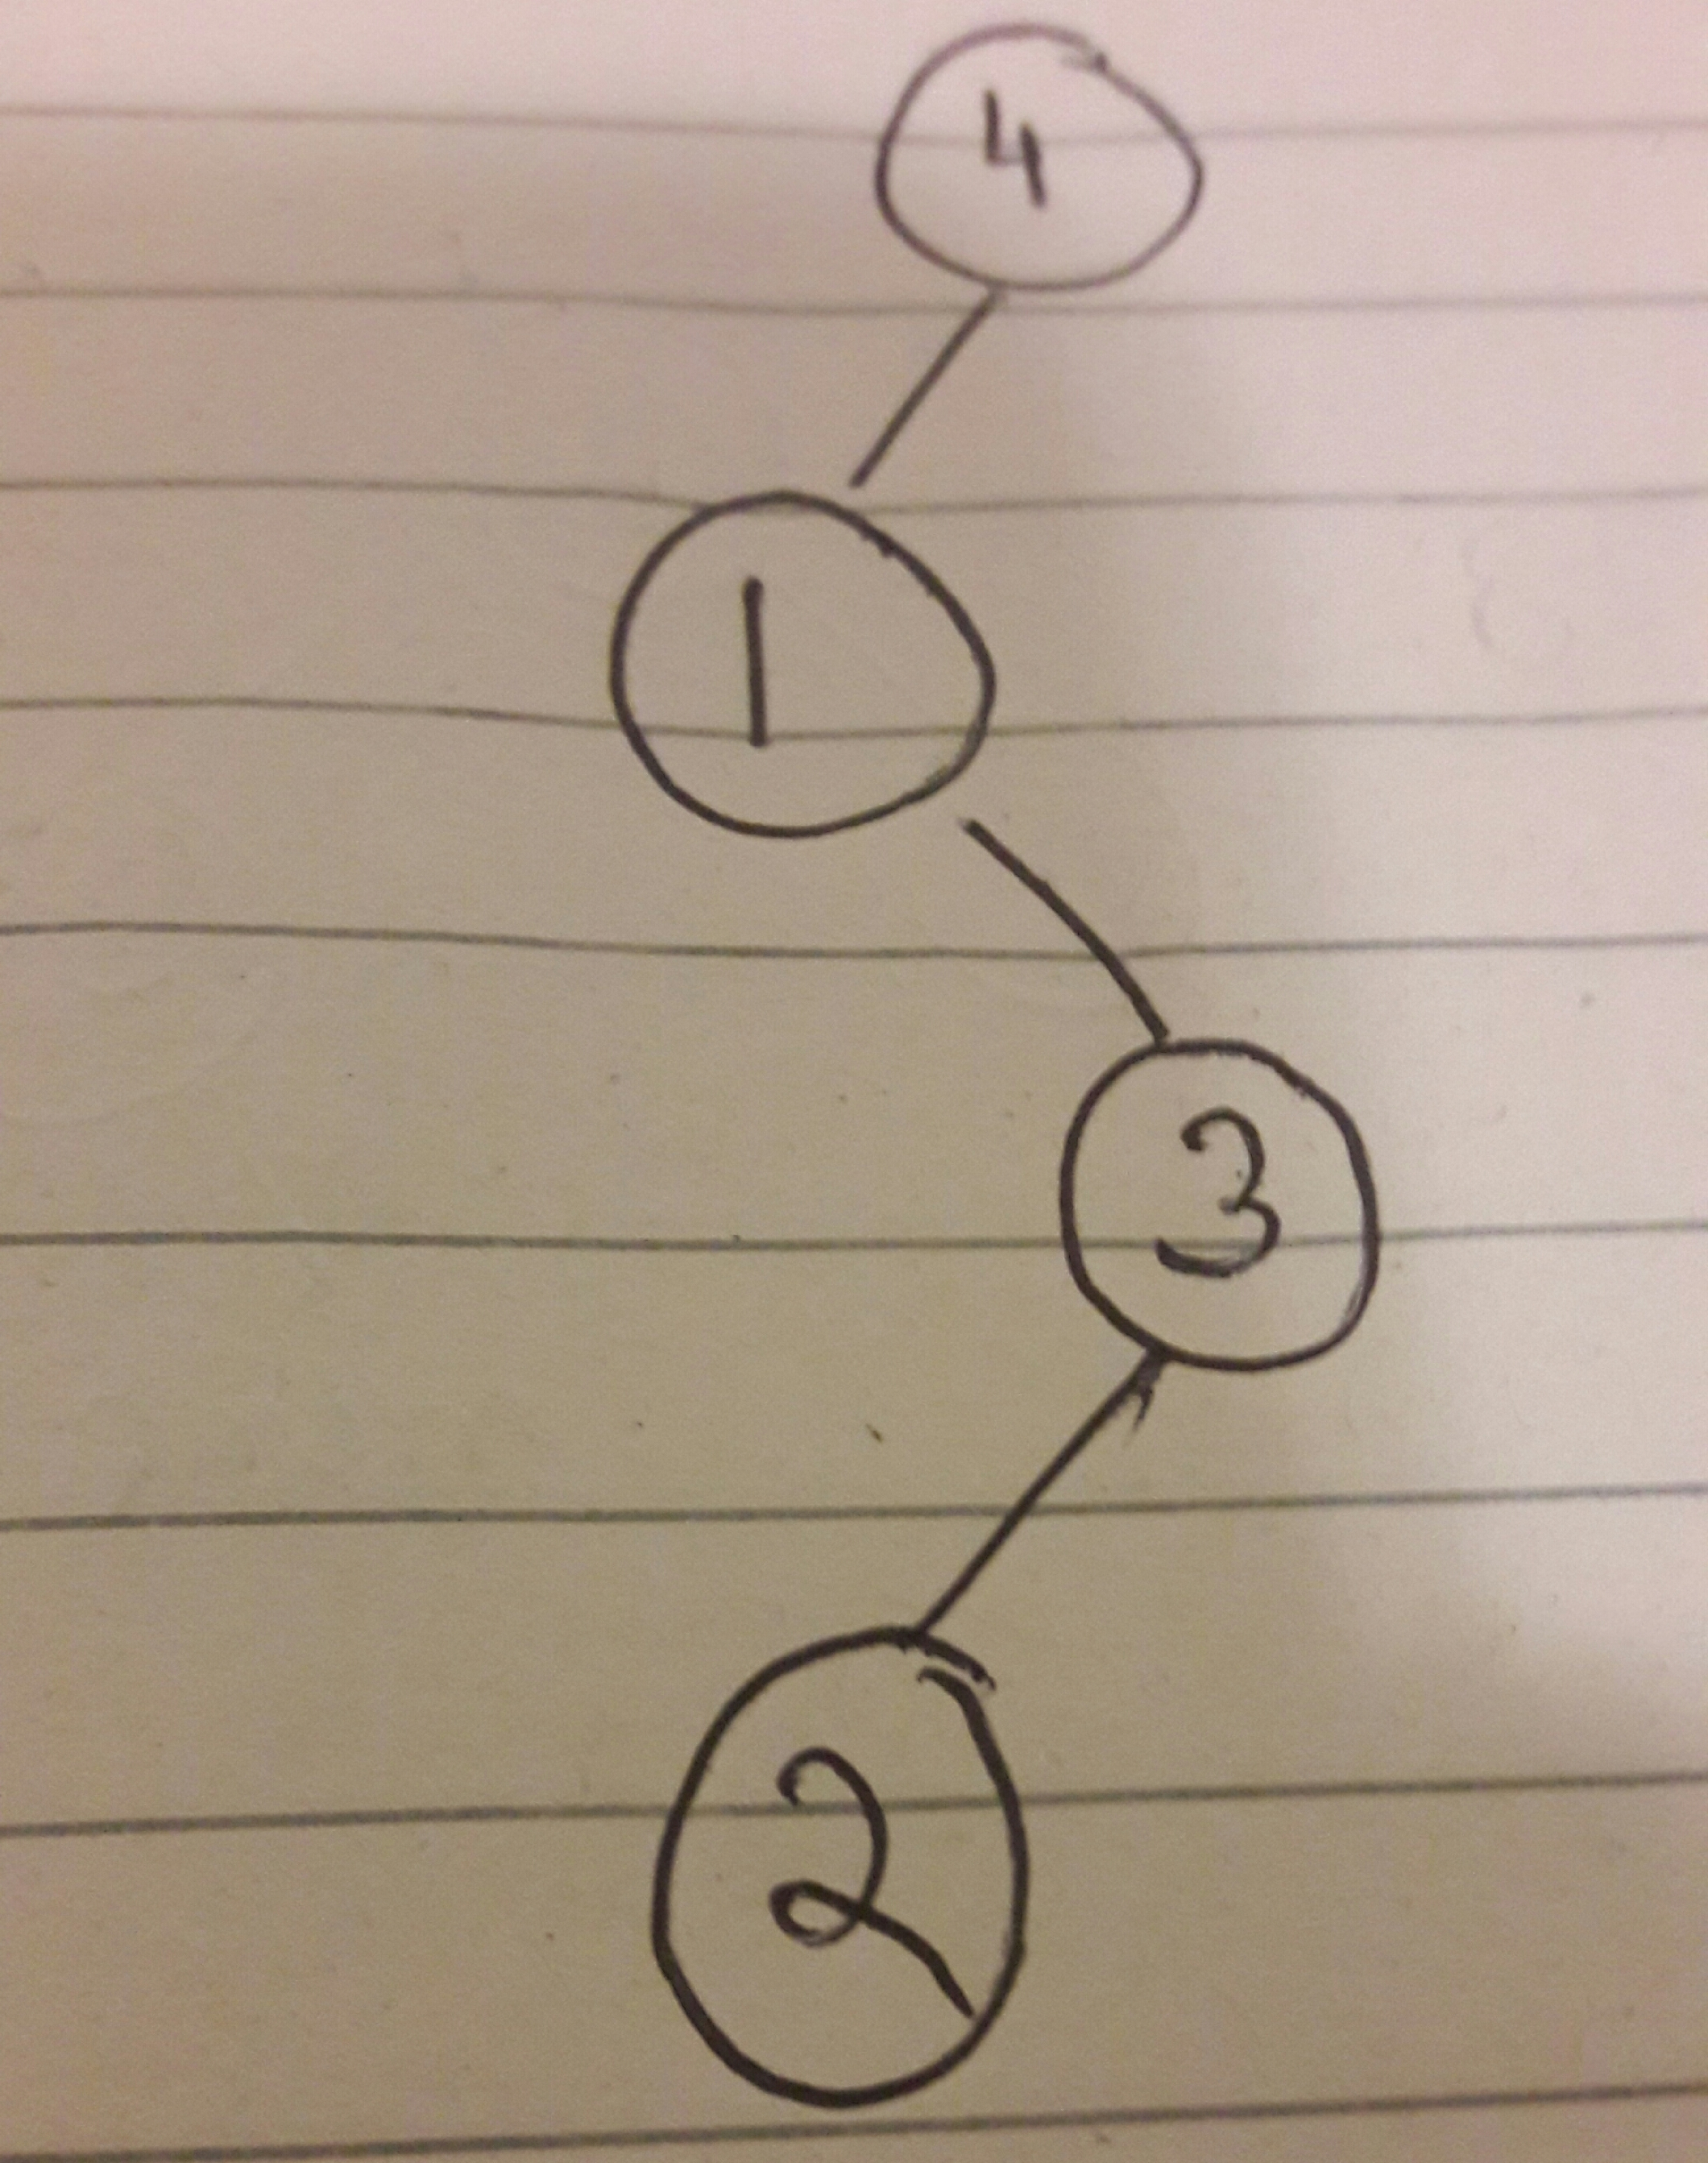
\includegraphics[scale=0.05]{6.jpg}




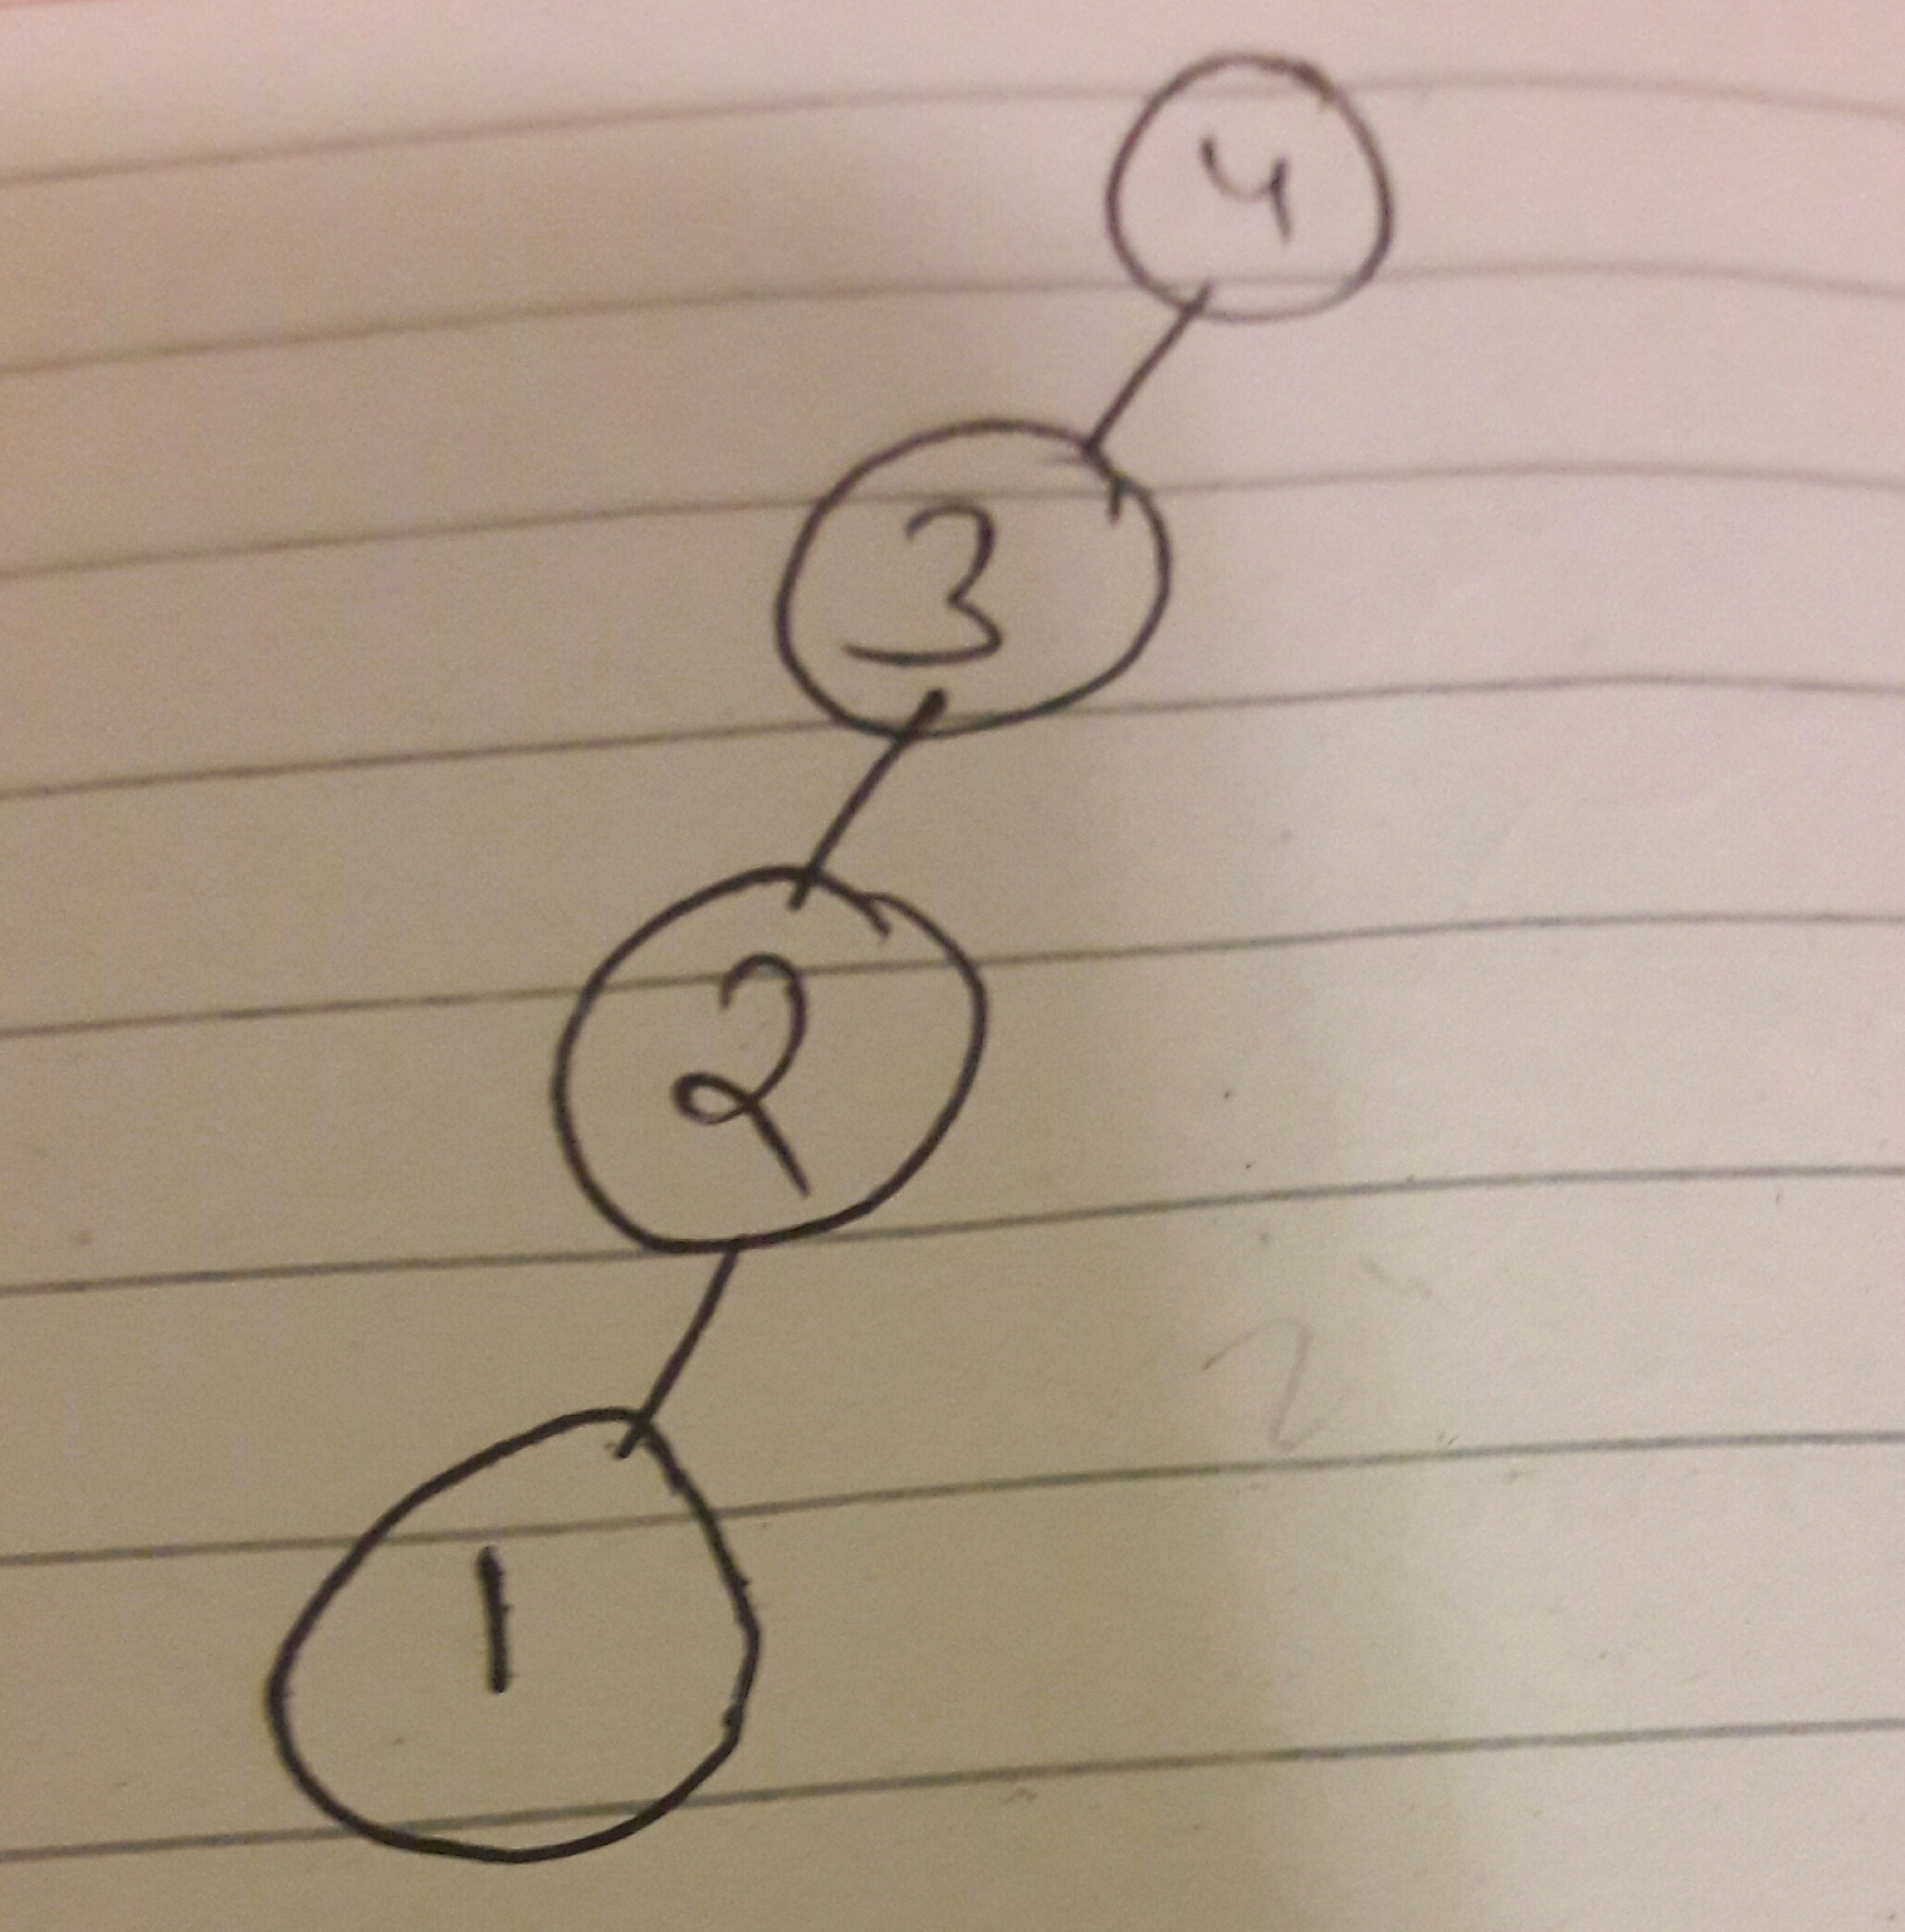
\includegraphics[scale=0.05]{7.jpg}



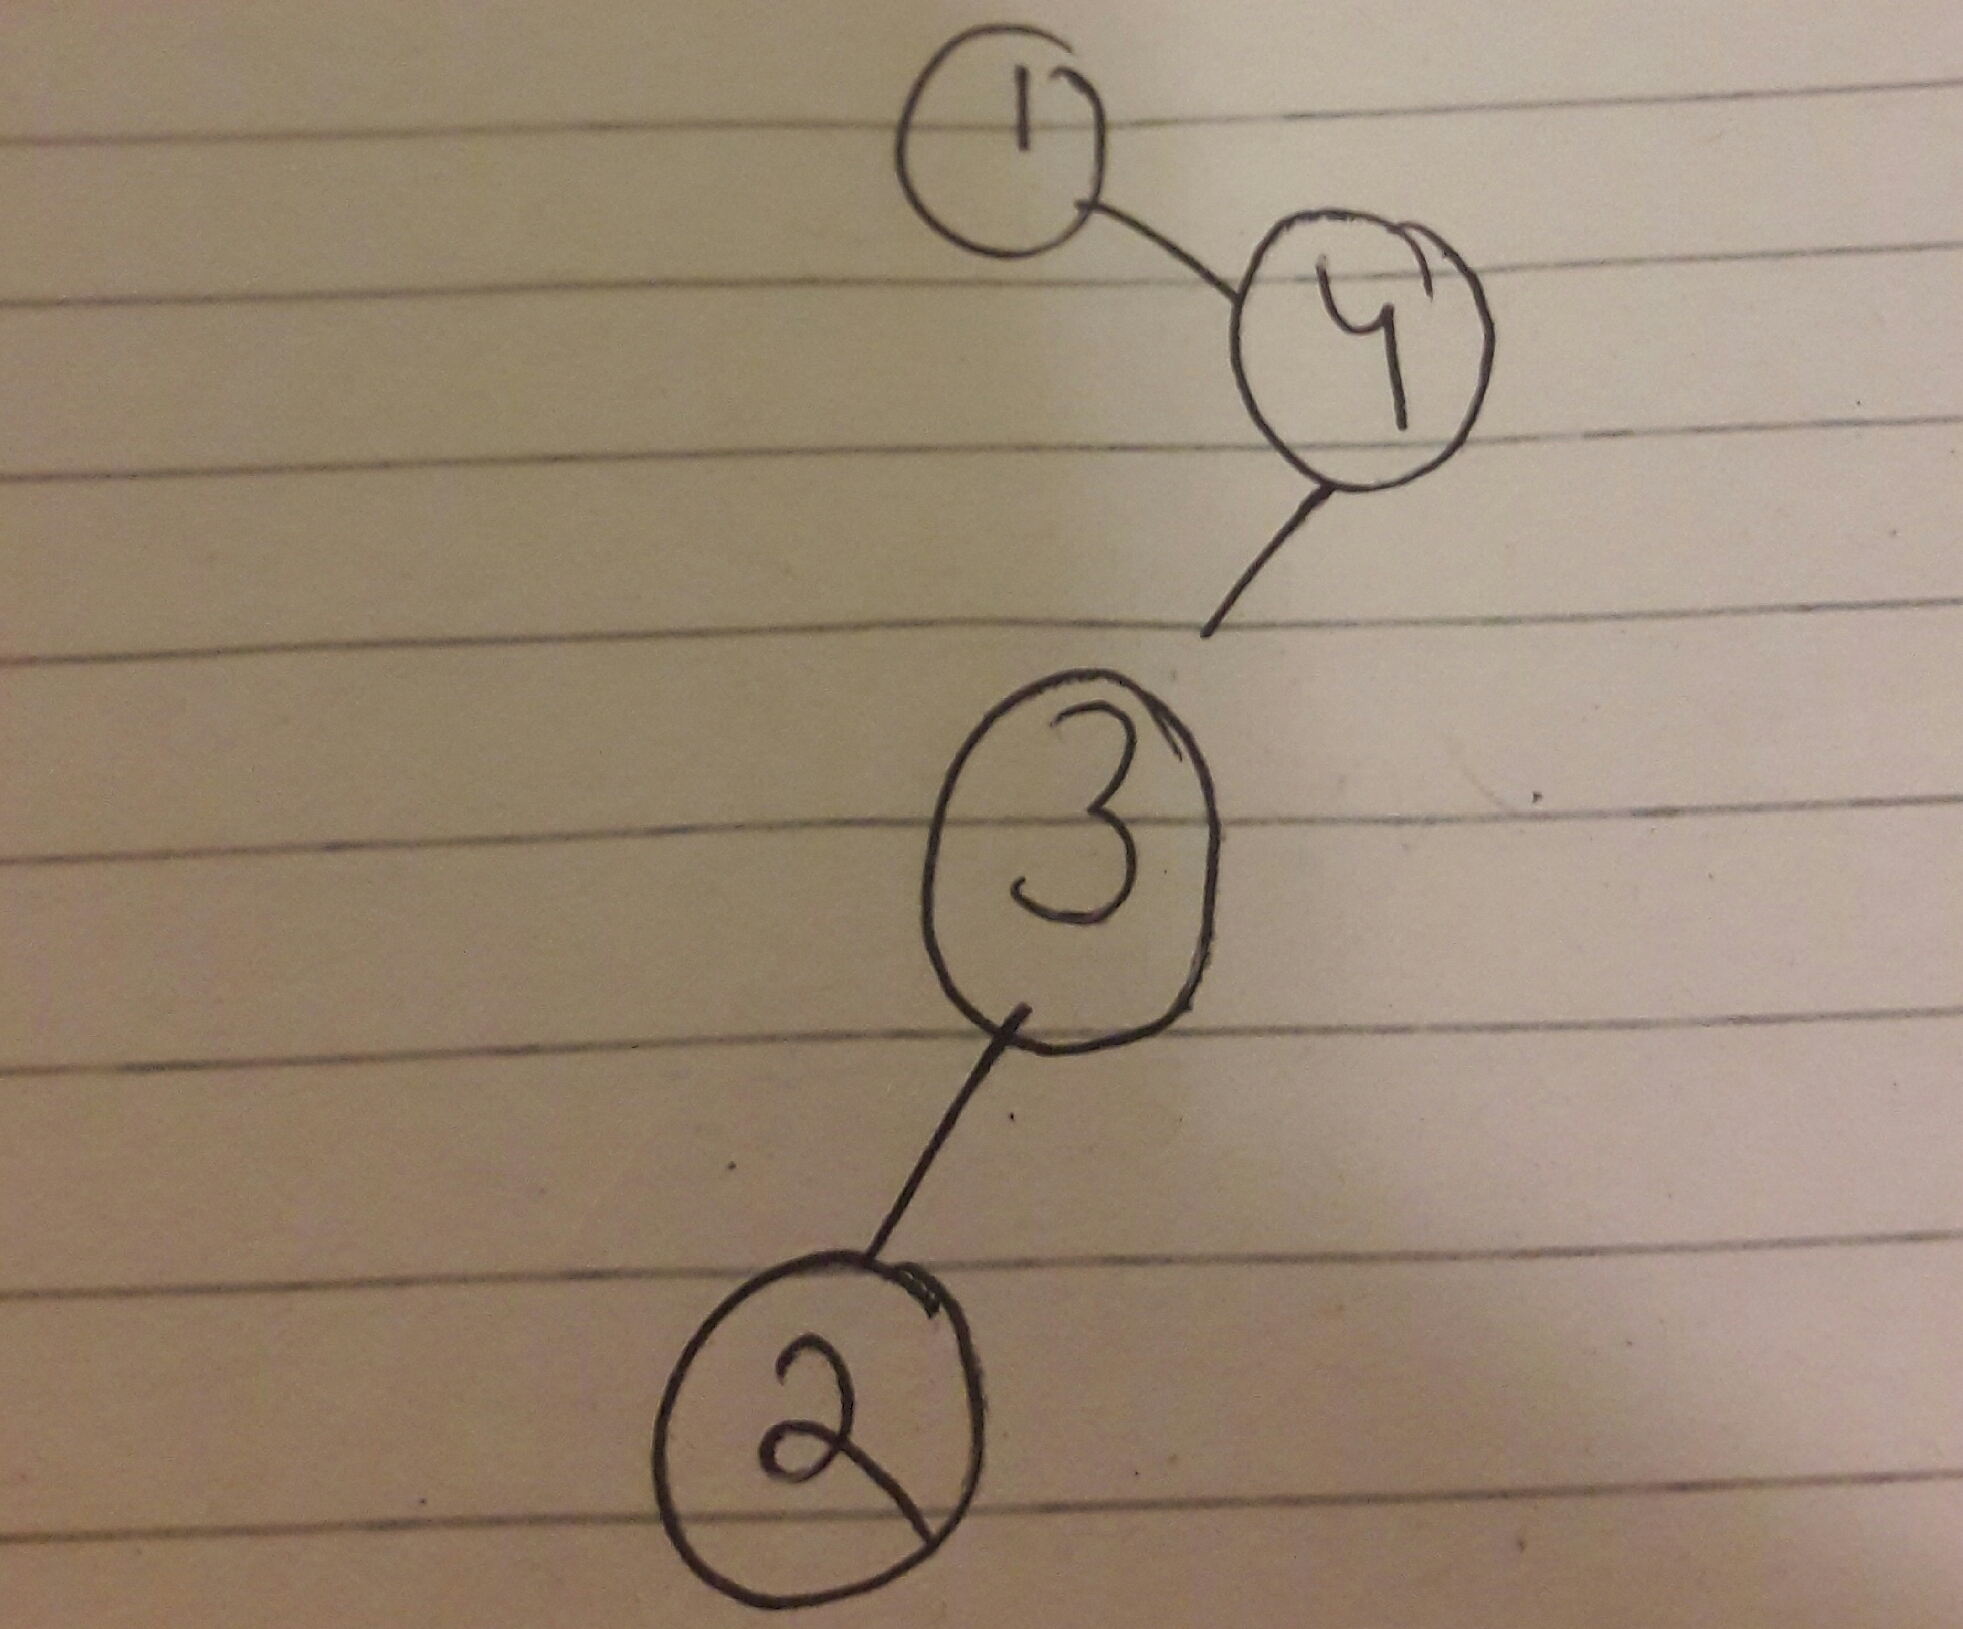
\includegraphics[scale=0.05]{8.jpg}




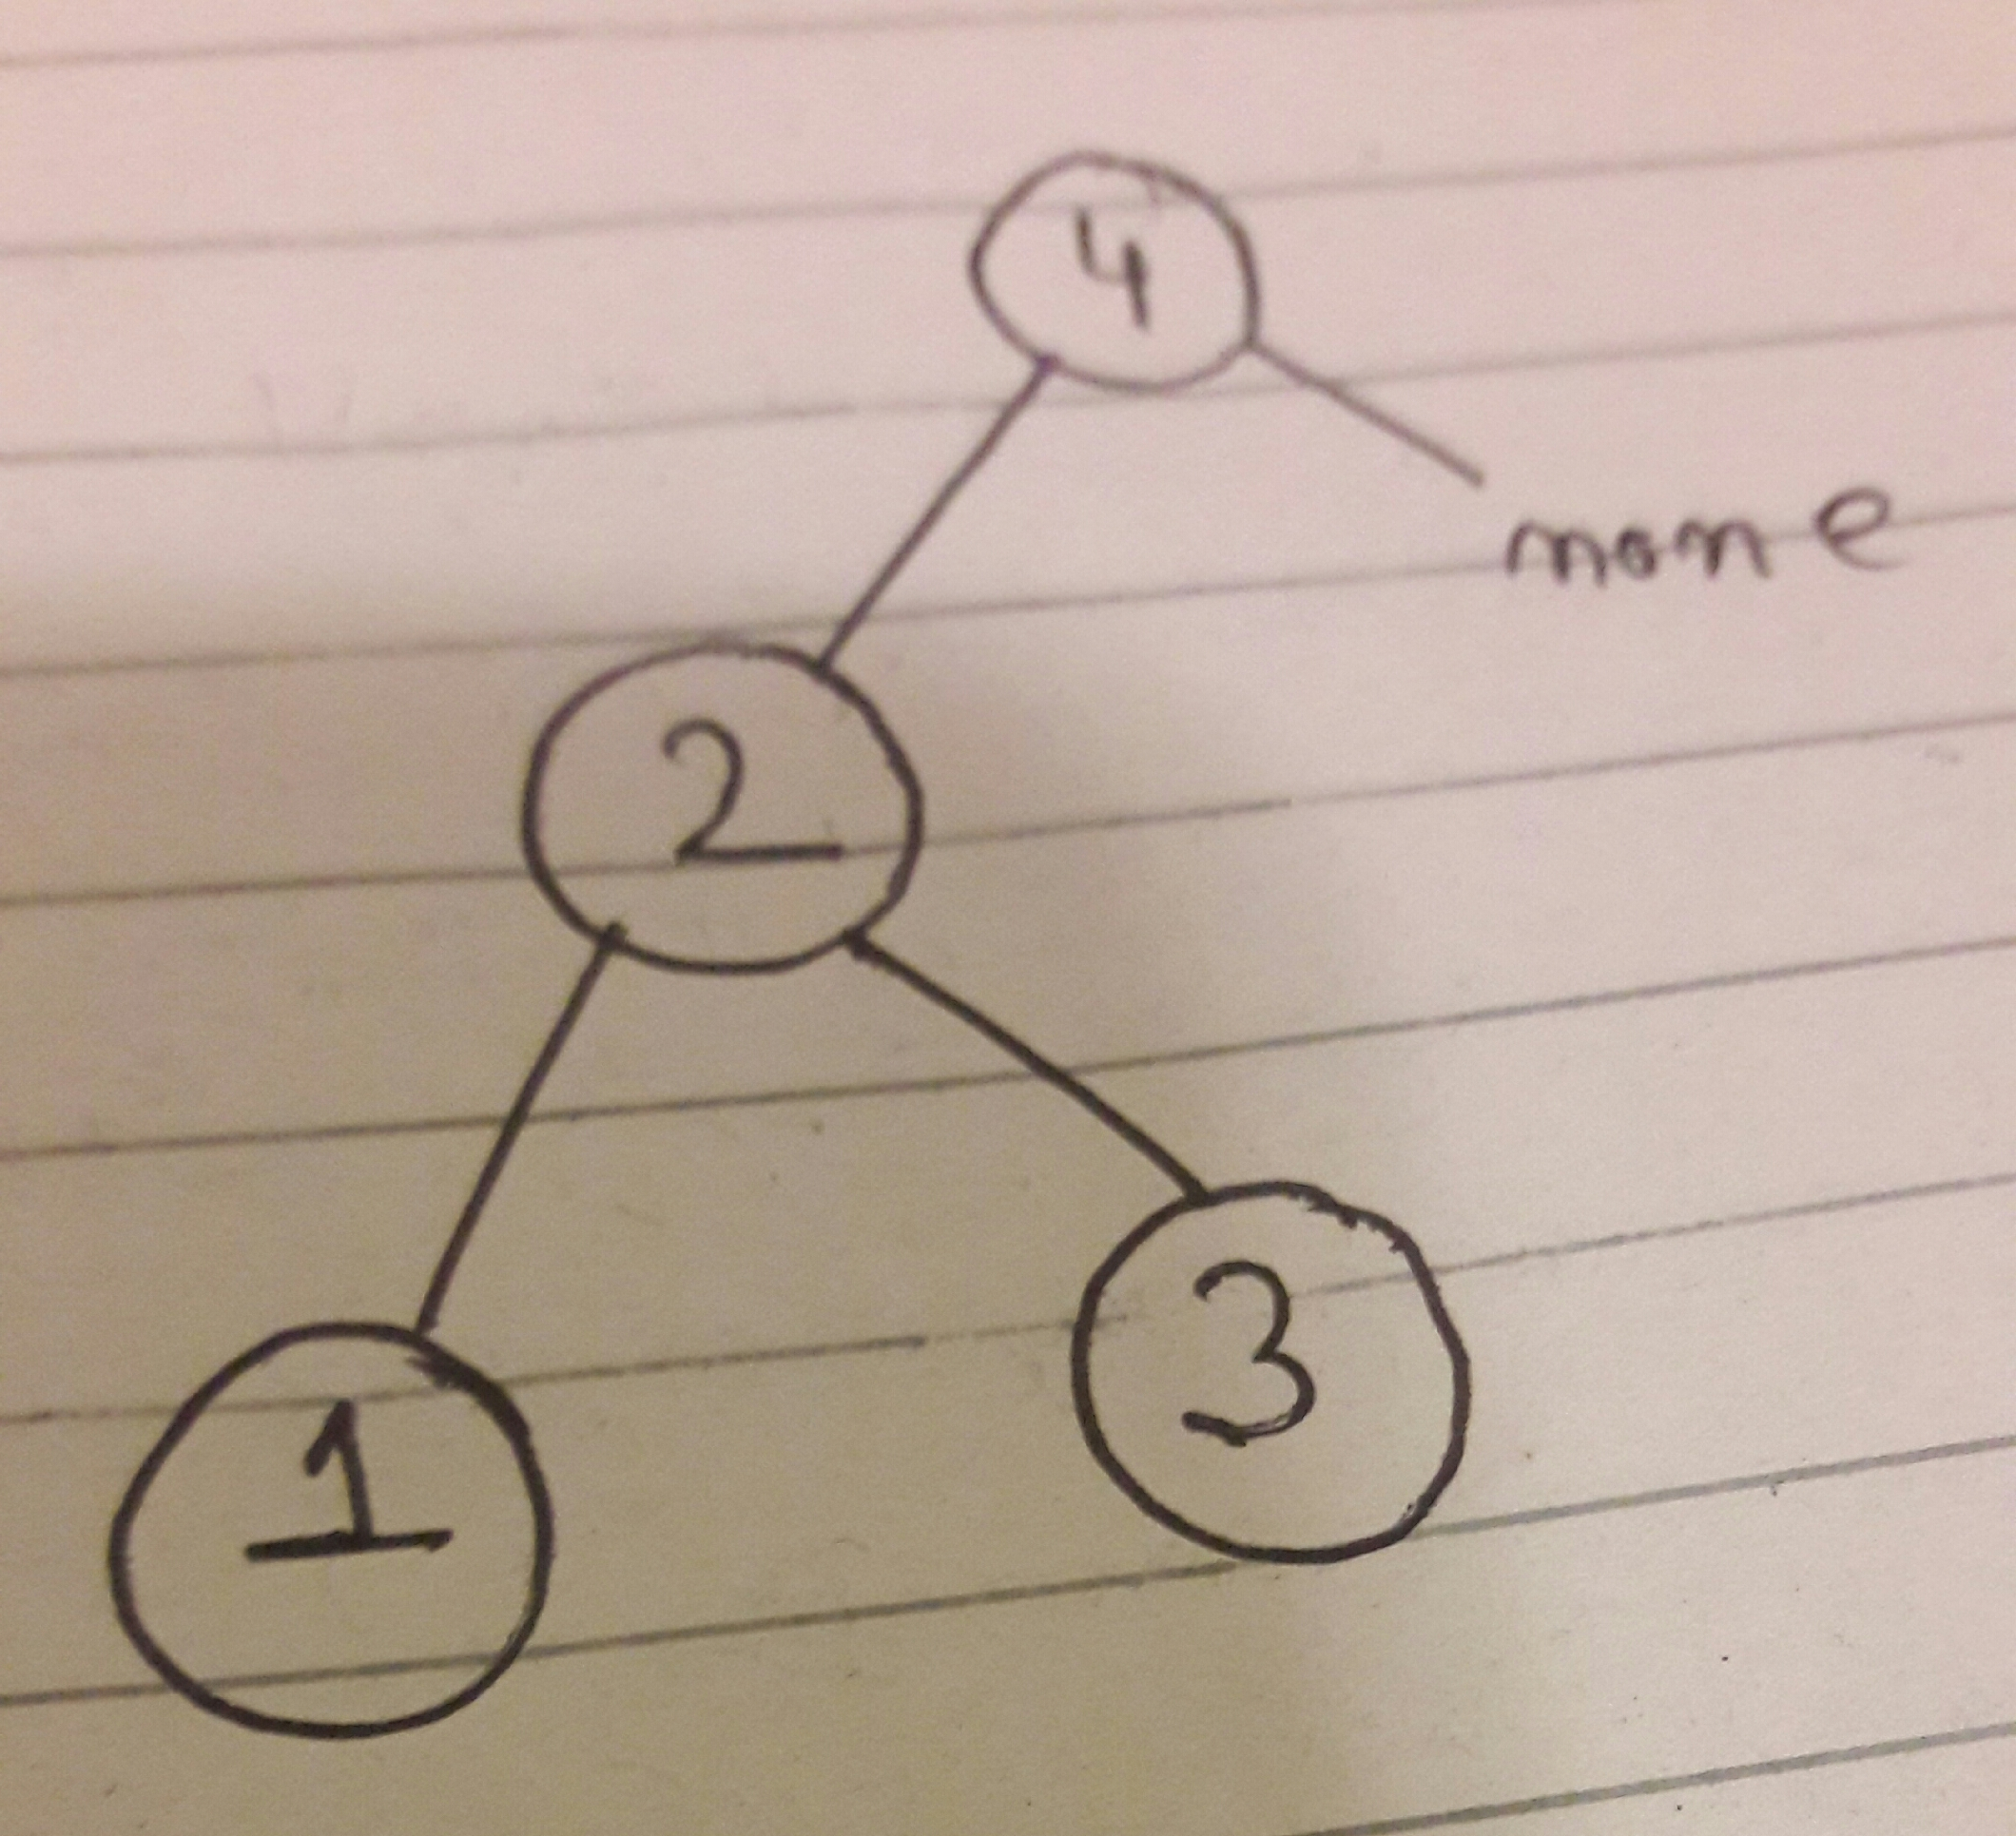
\includegraphics[scale=0.05]{9.jpg}




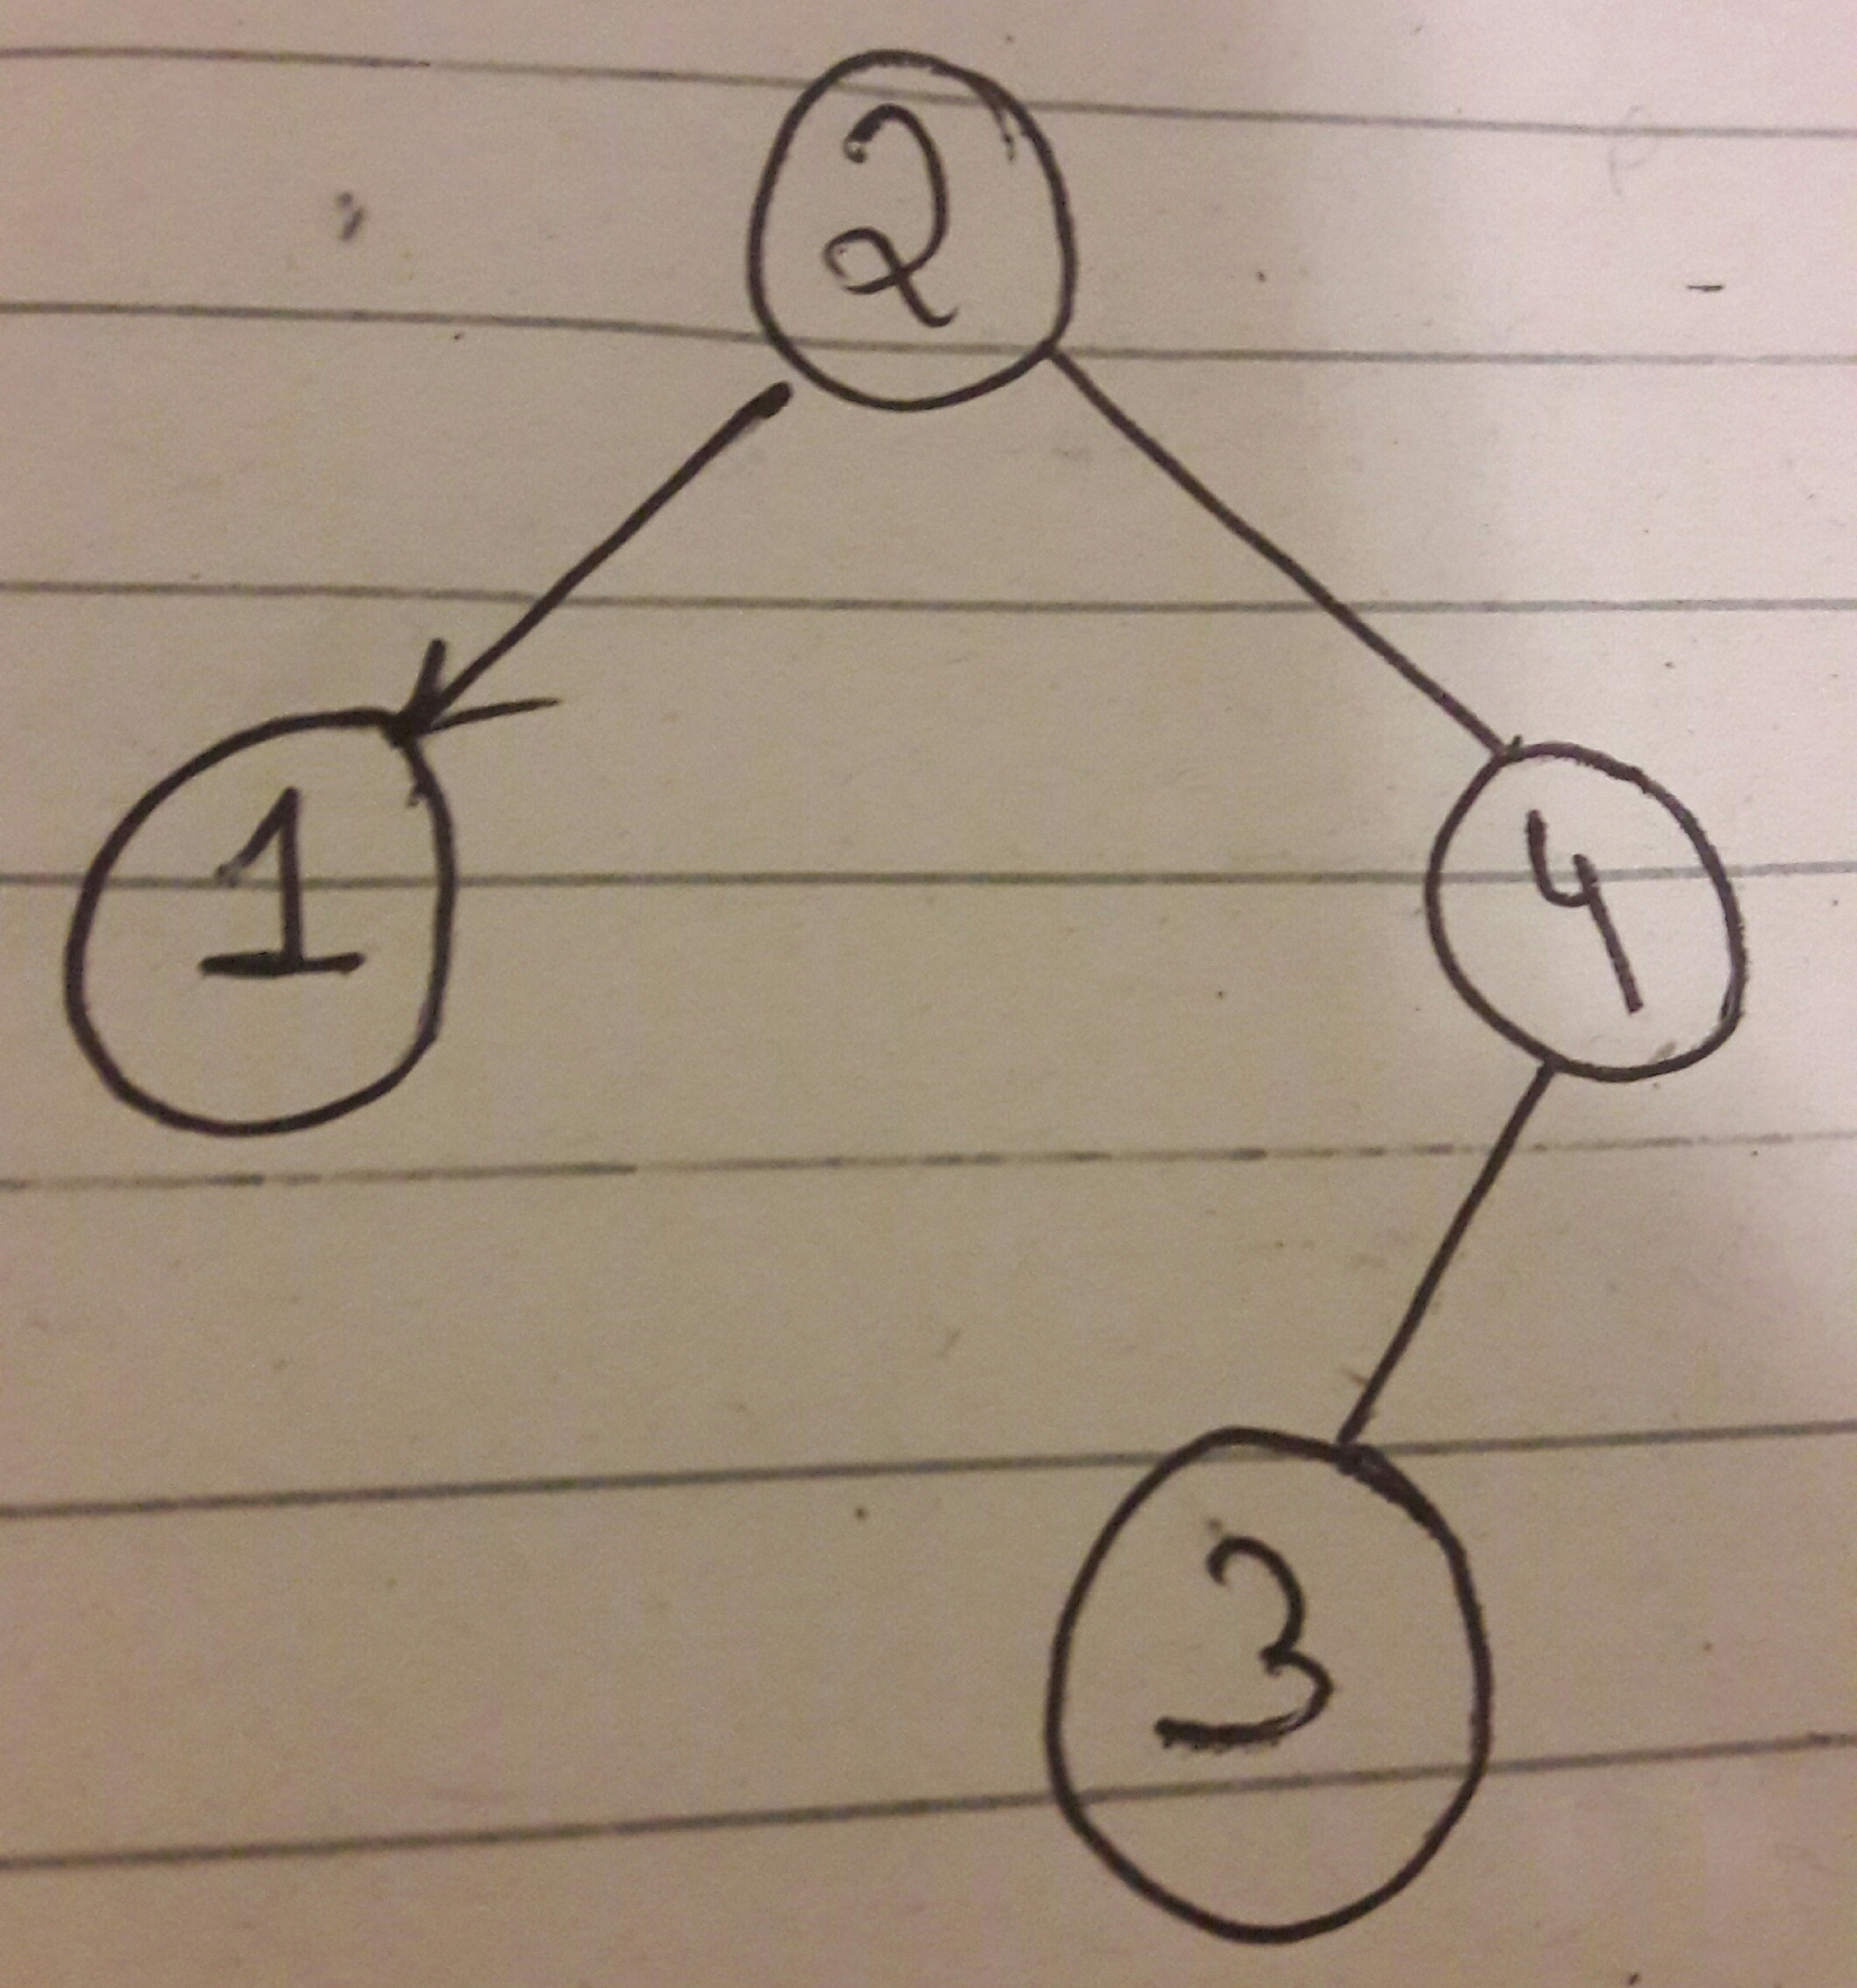
\includegraphics[scale=0.05]{10.jpg}




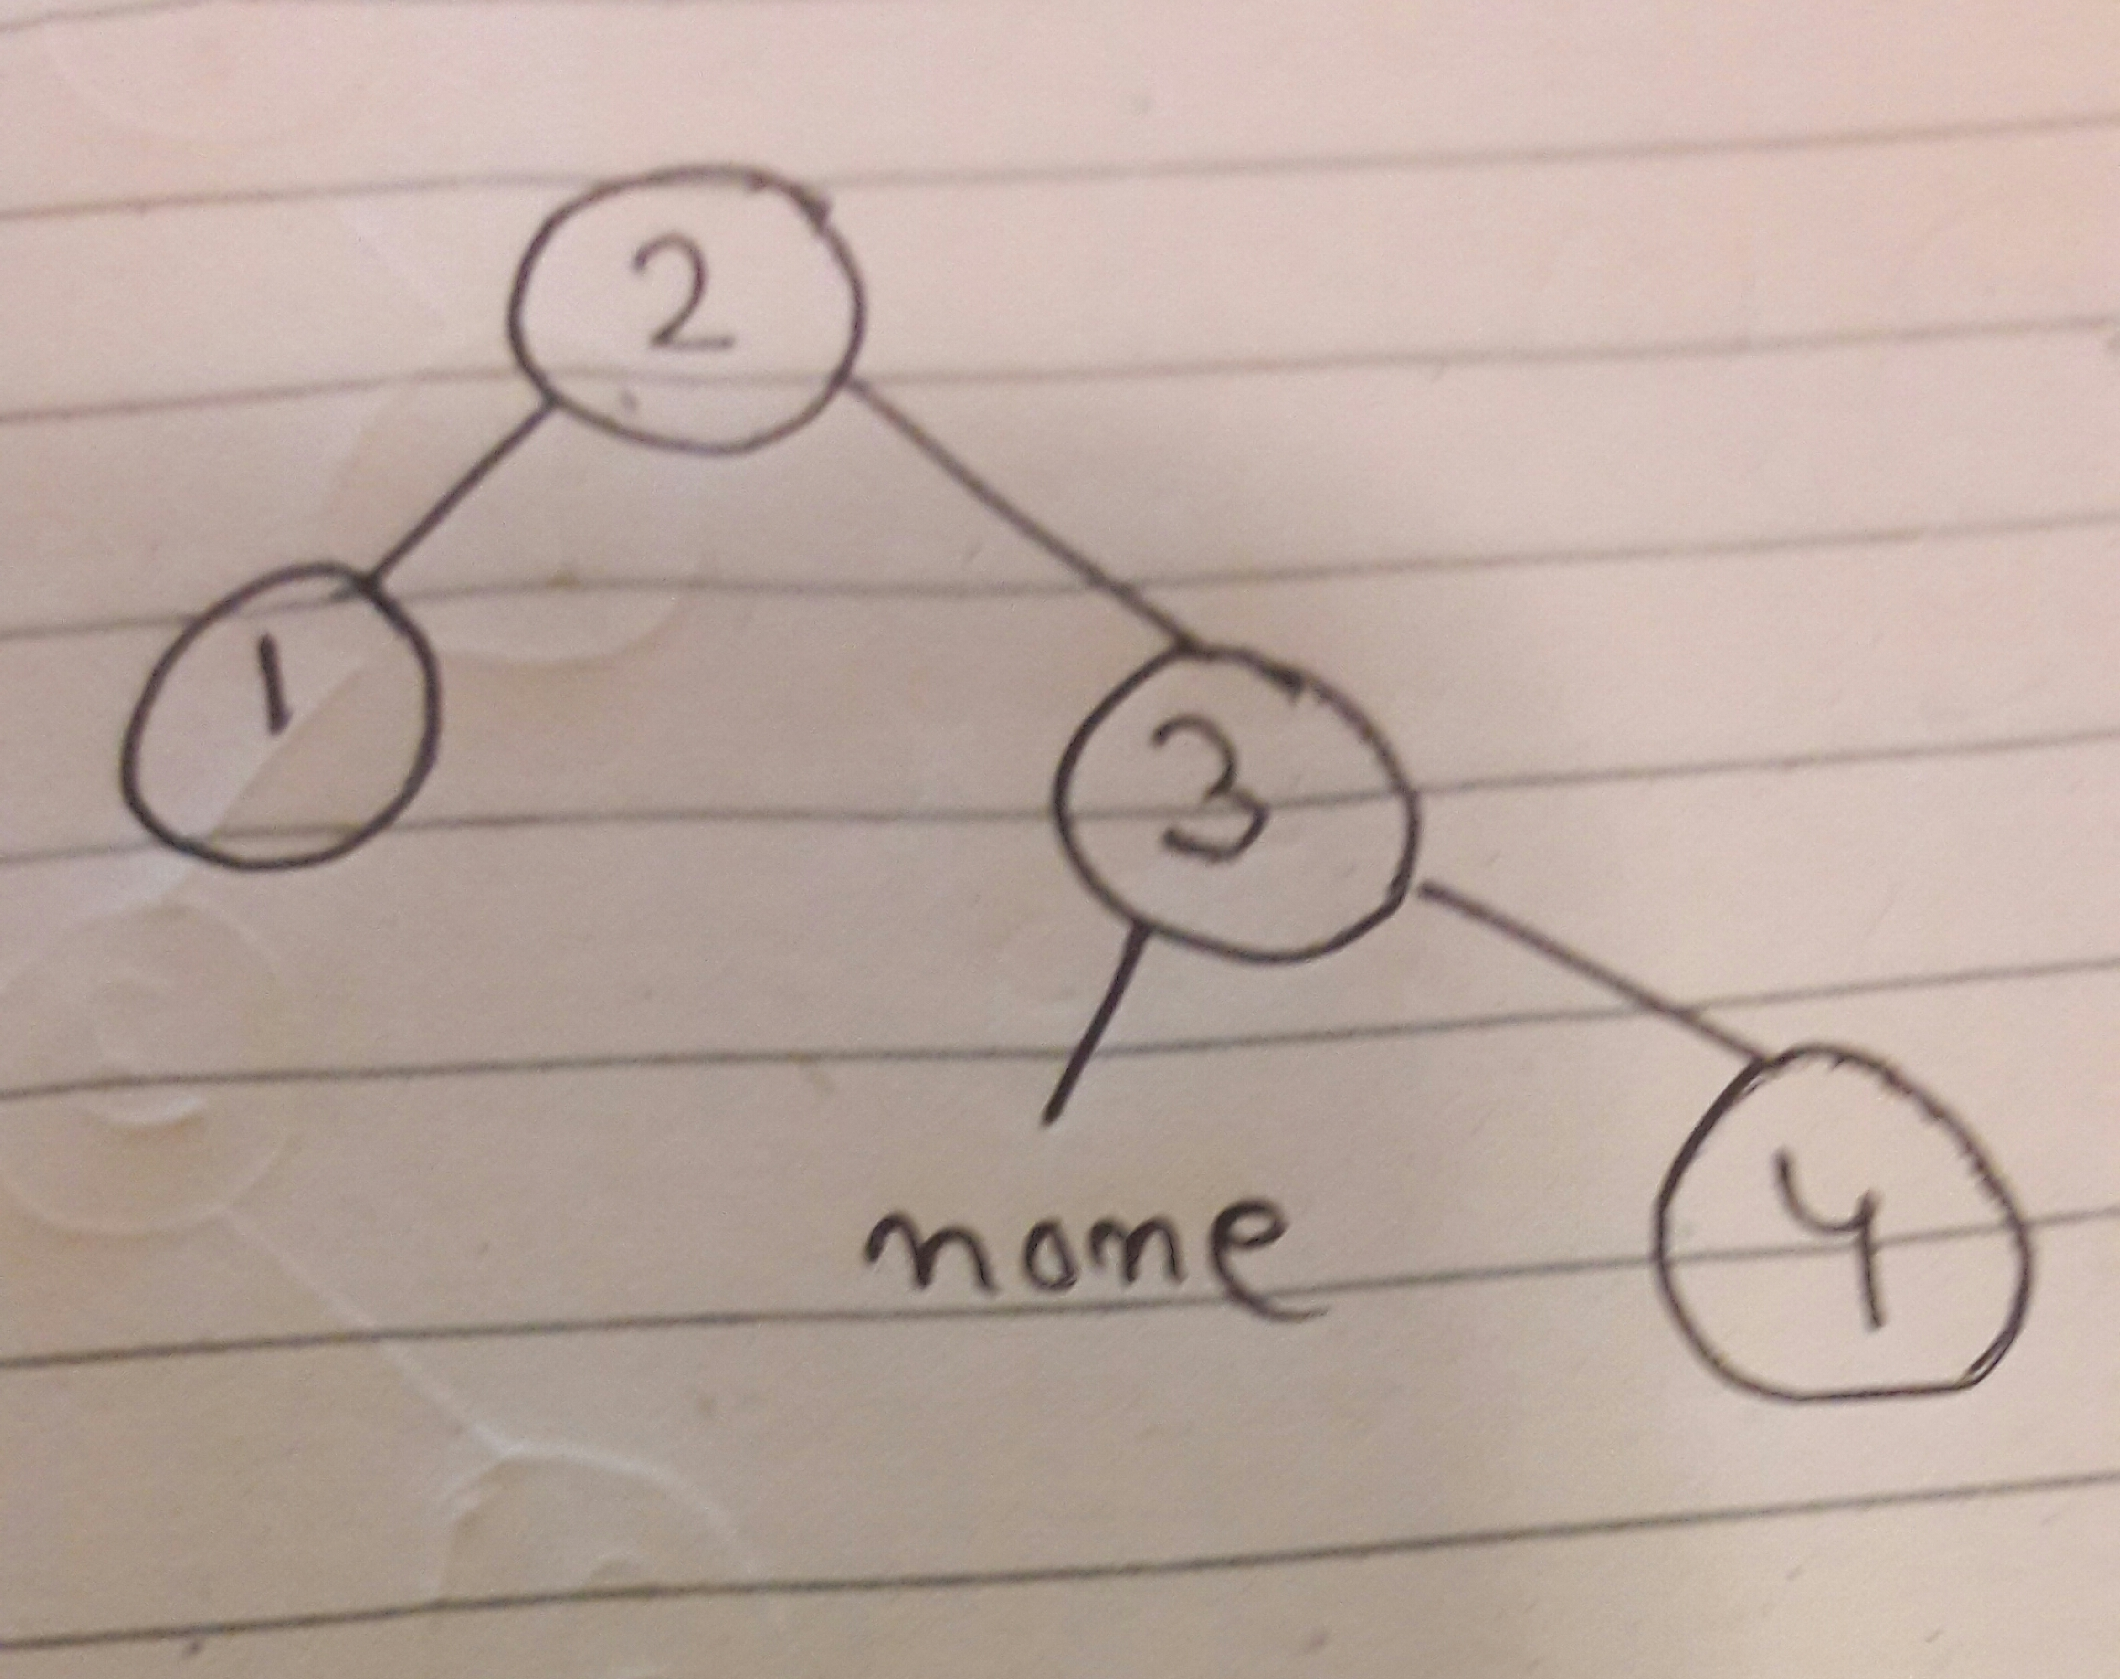
\includegraphics[scale=0.05]{11.jpg}




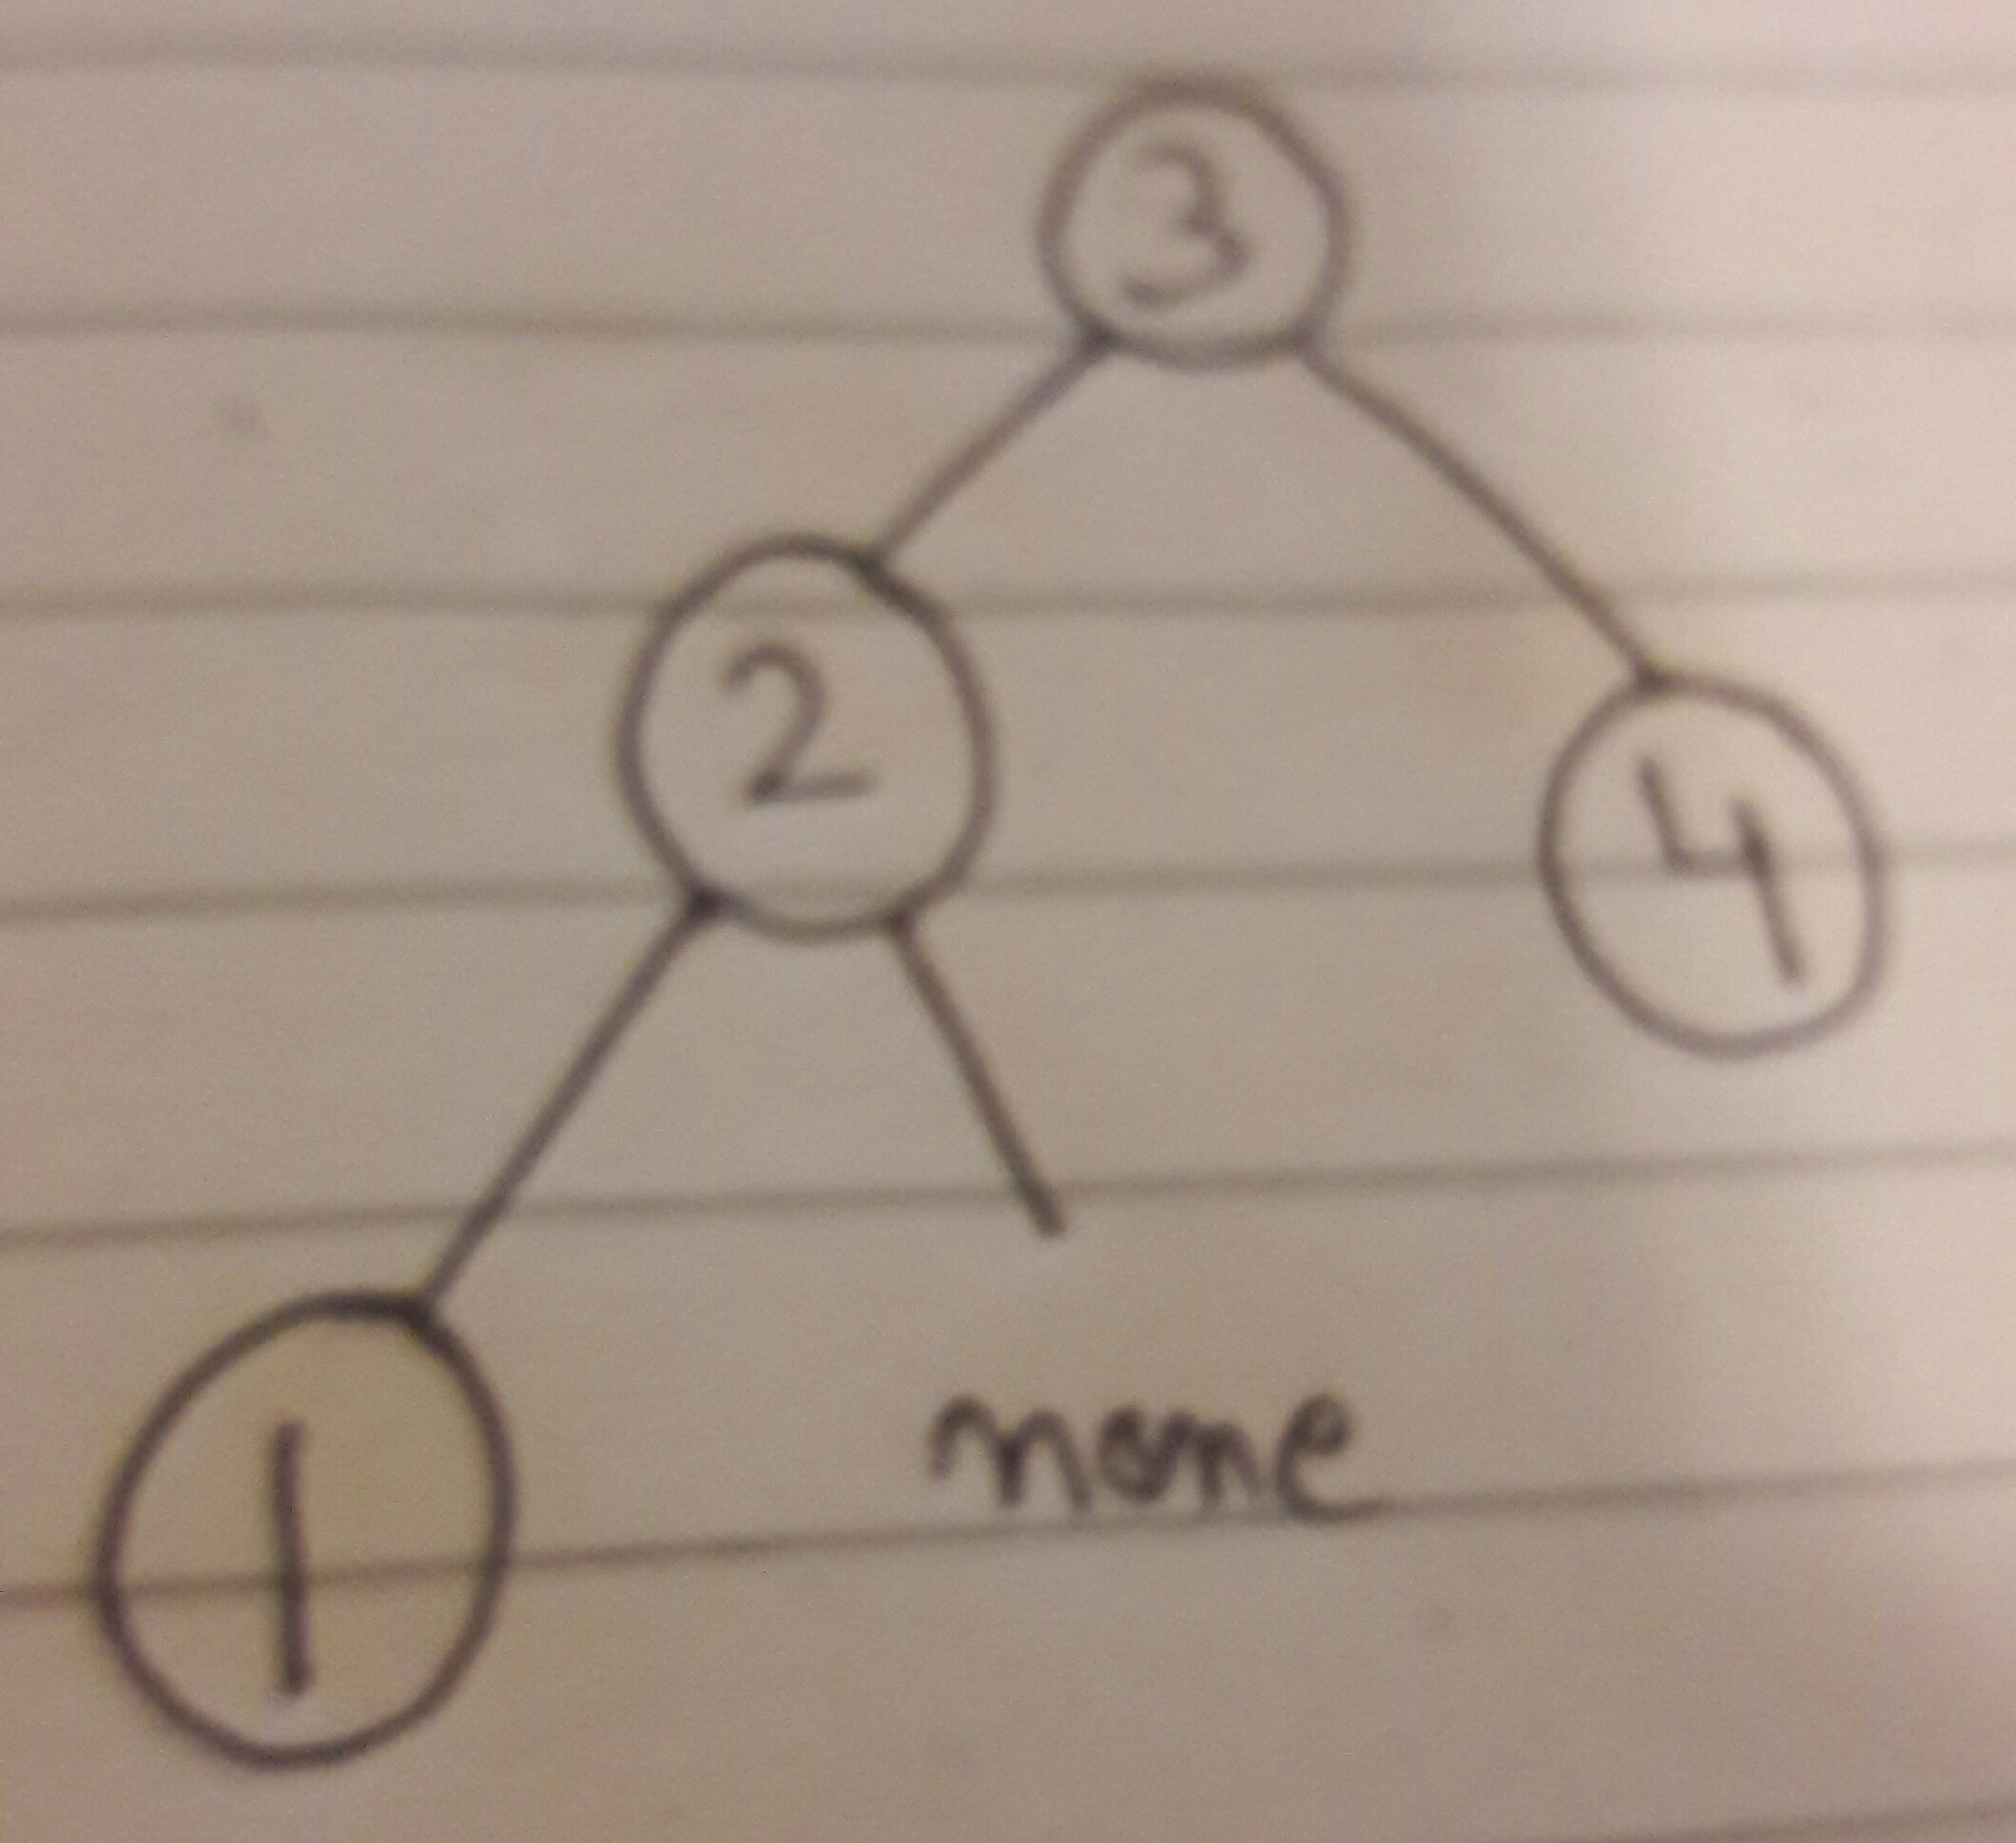
\includegraphics[scale=0.05]{12.jpg}



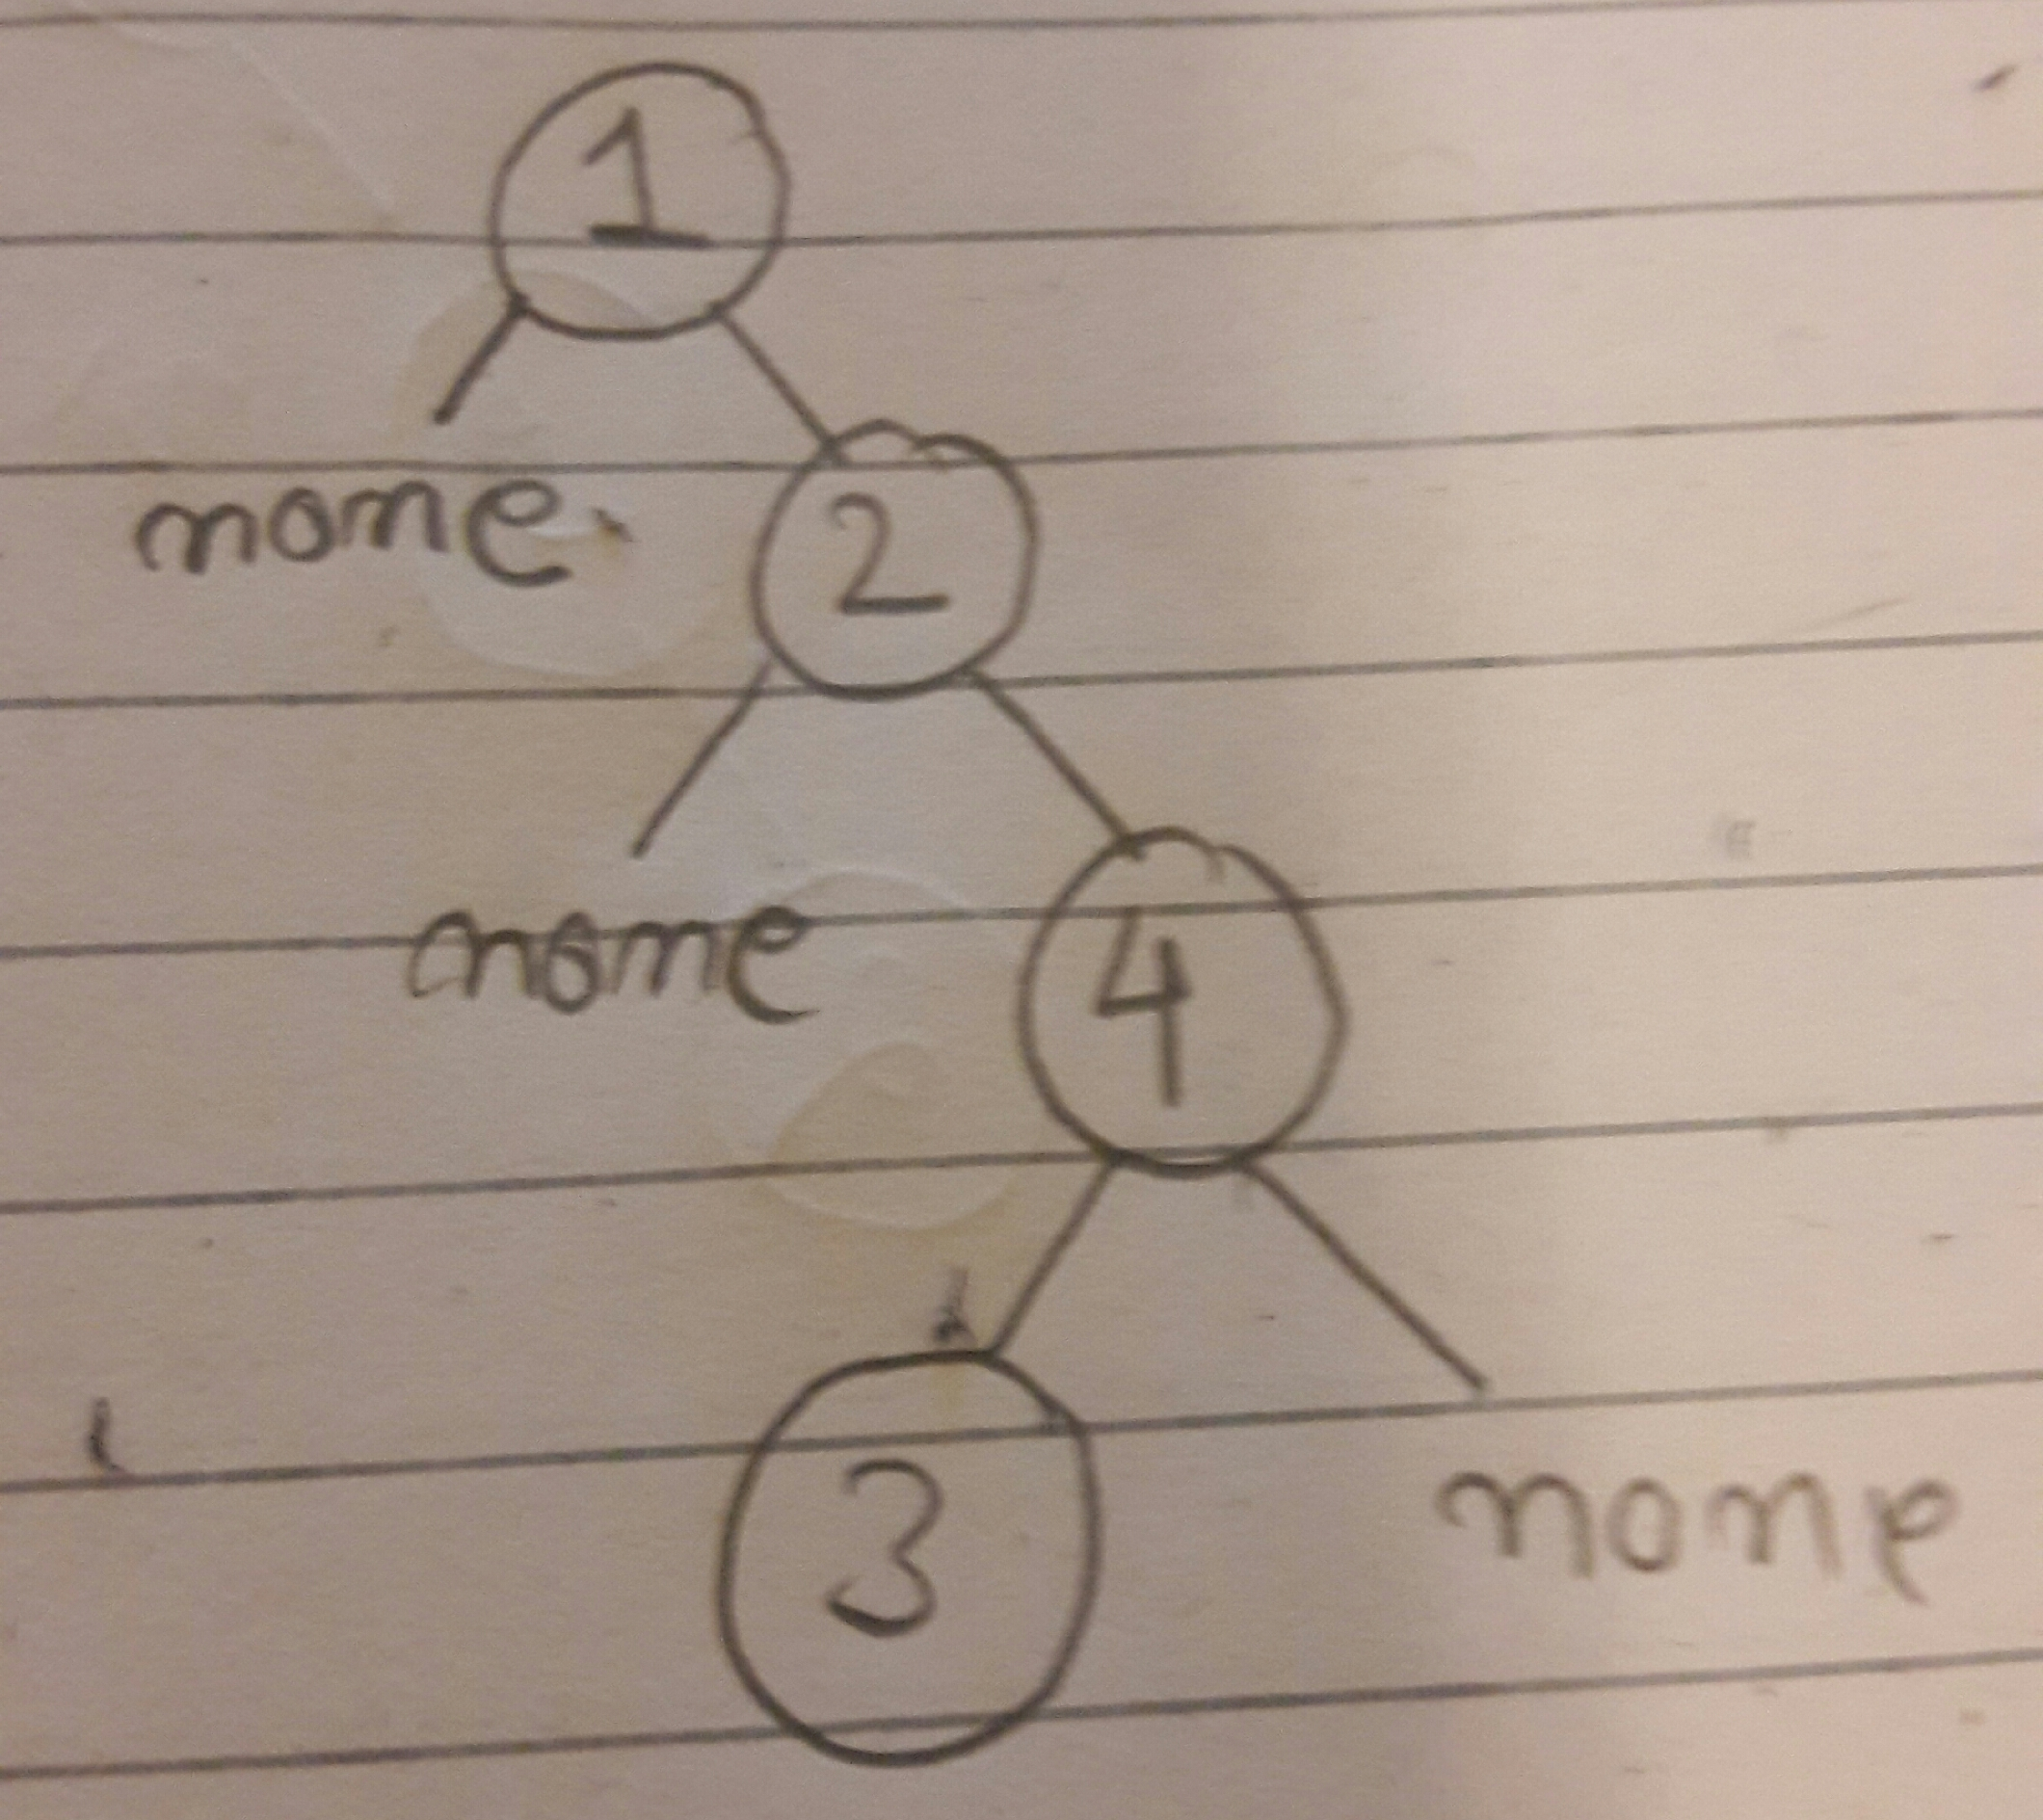
\includegraphics[scale=0.05]{13.jpg}





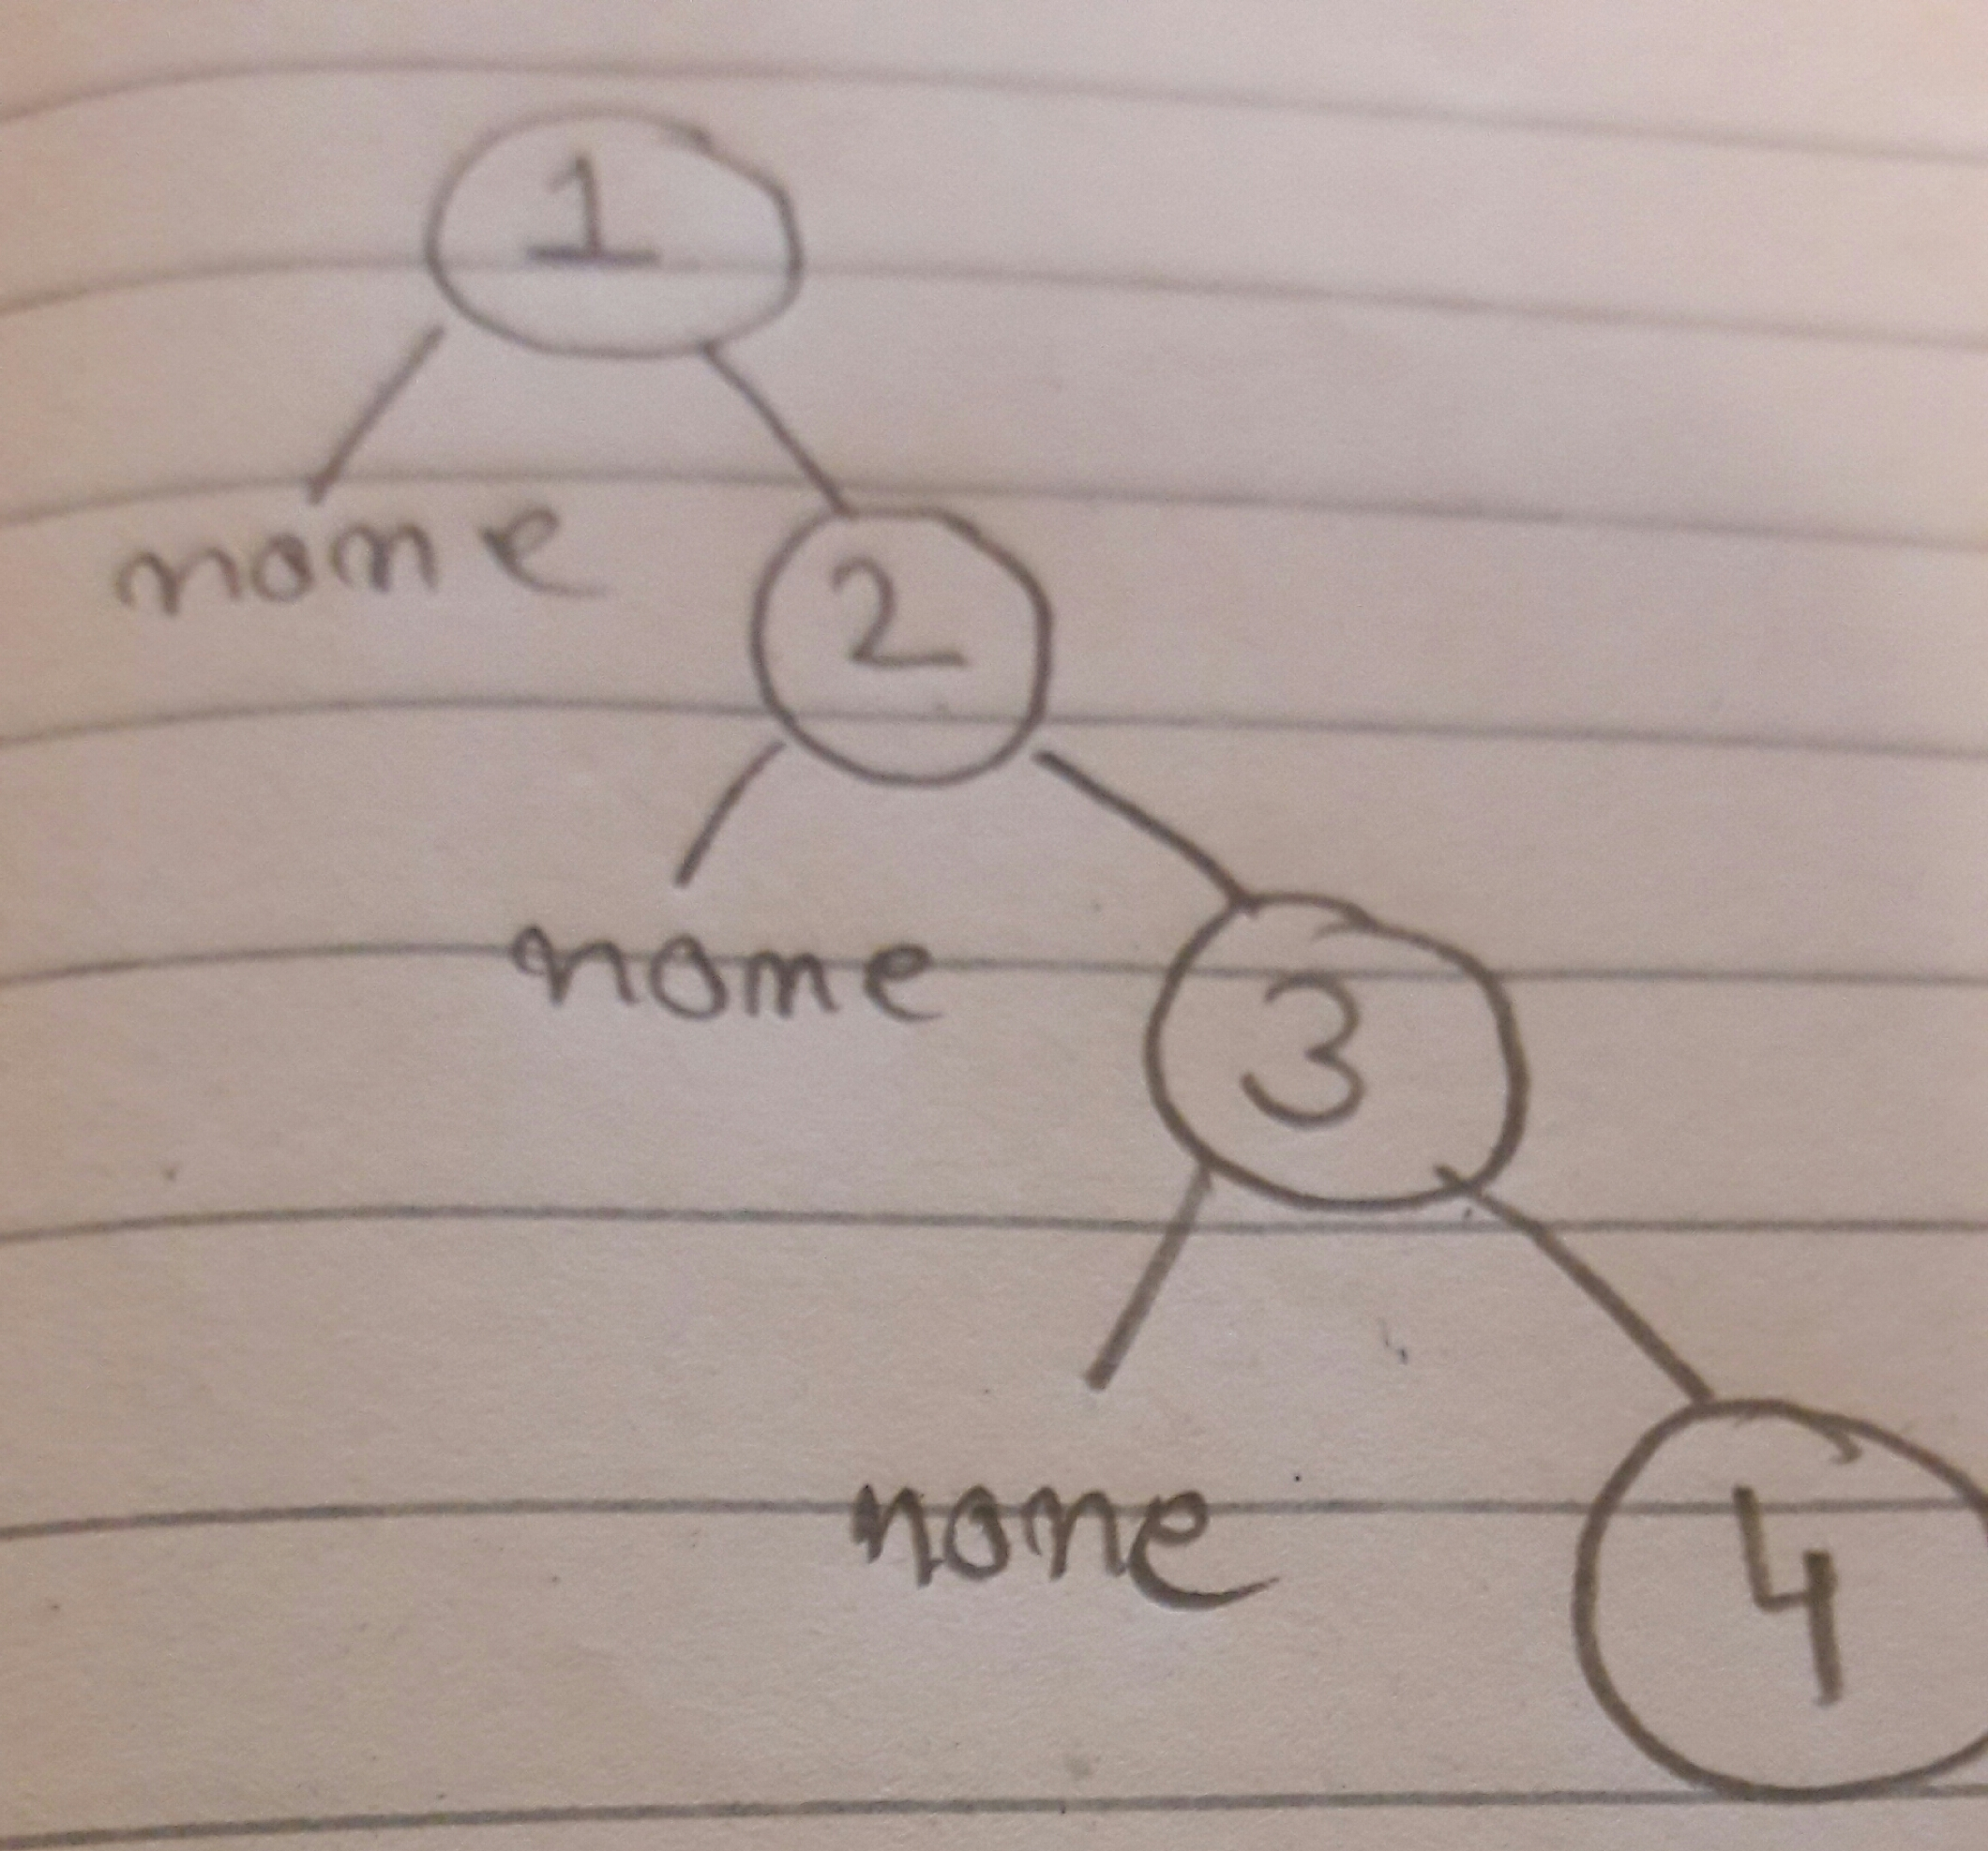
\includegraphics[scale=0.05]{14.jpg}




\section*{Question 2}
The final binary tree is:




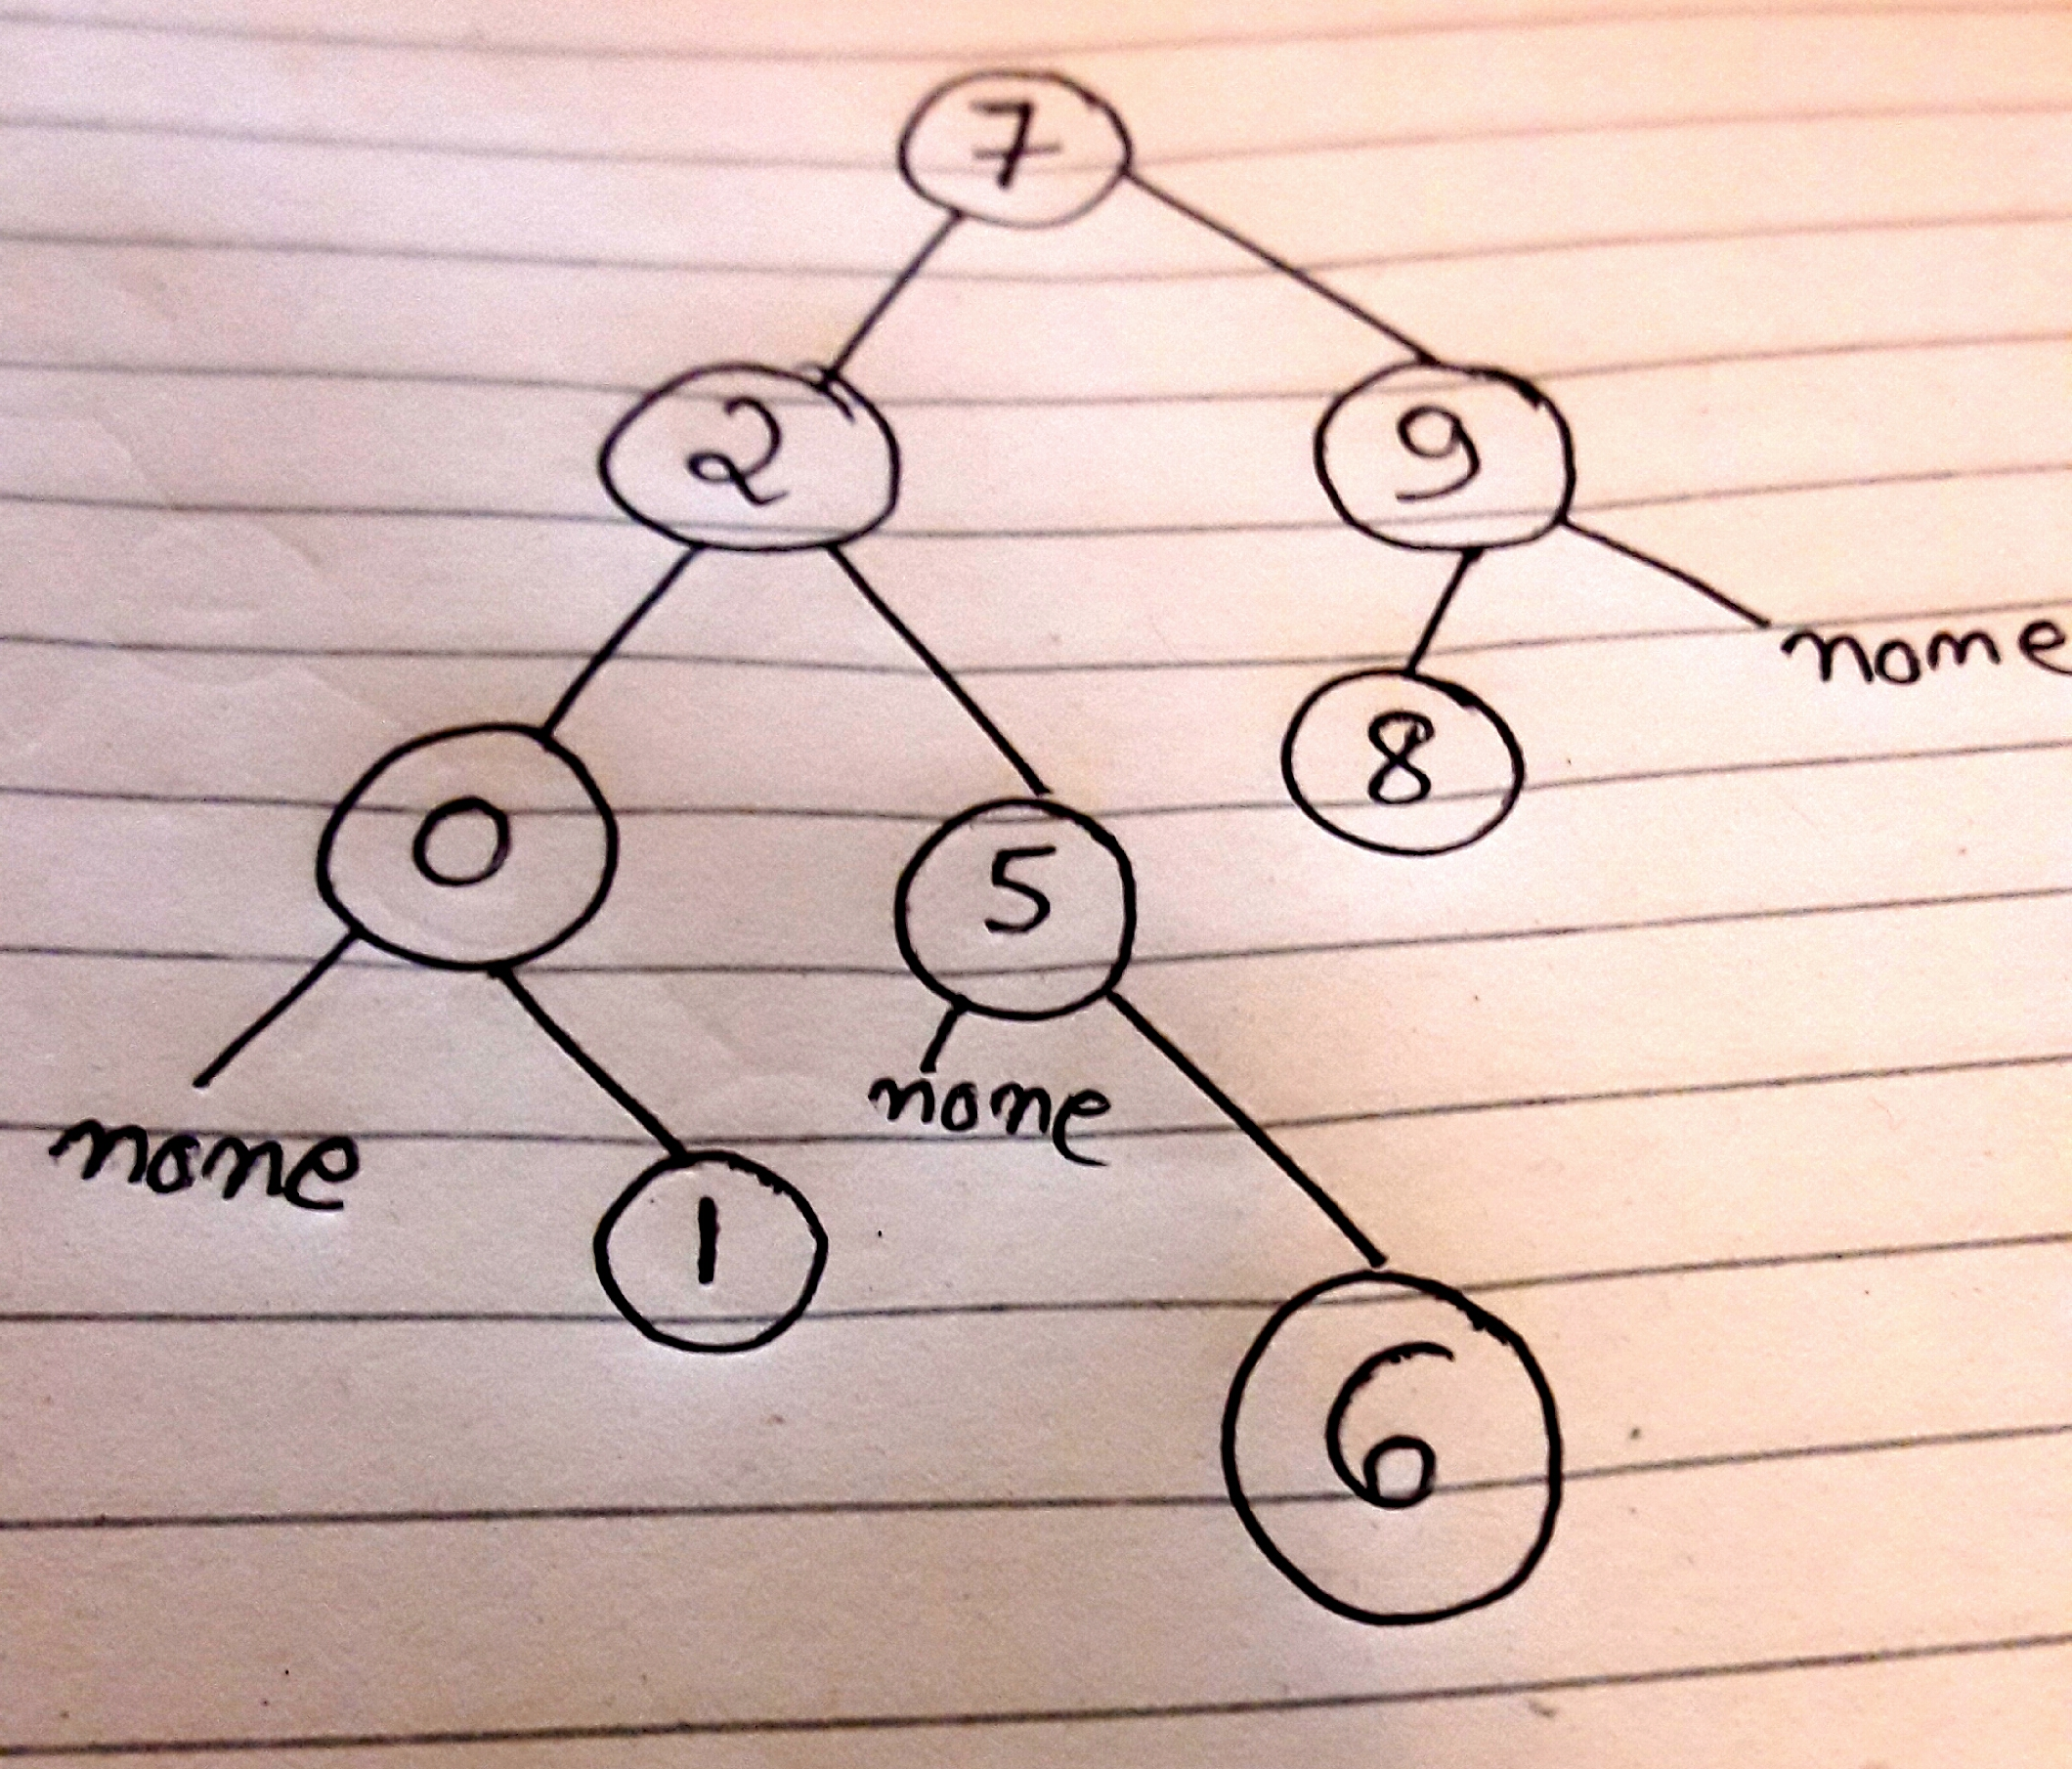
\includegraphics[scale=0.1]{15.jpg}



\section*{Question 3}

After adding first 4 strings:

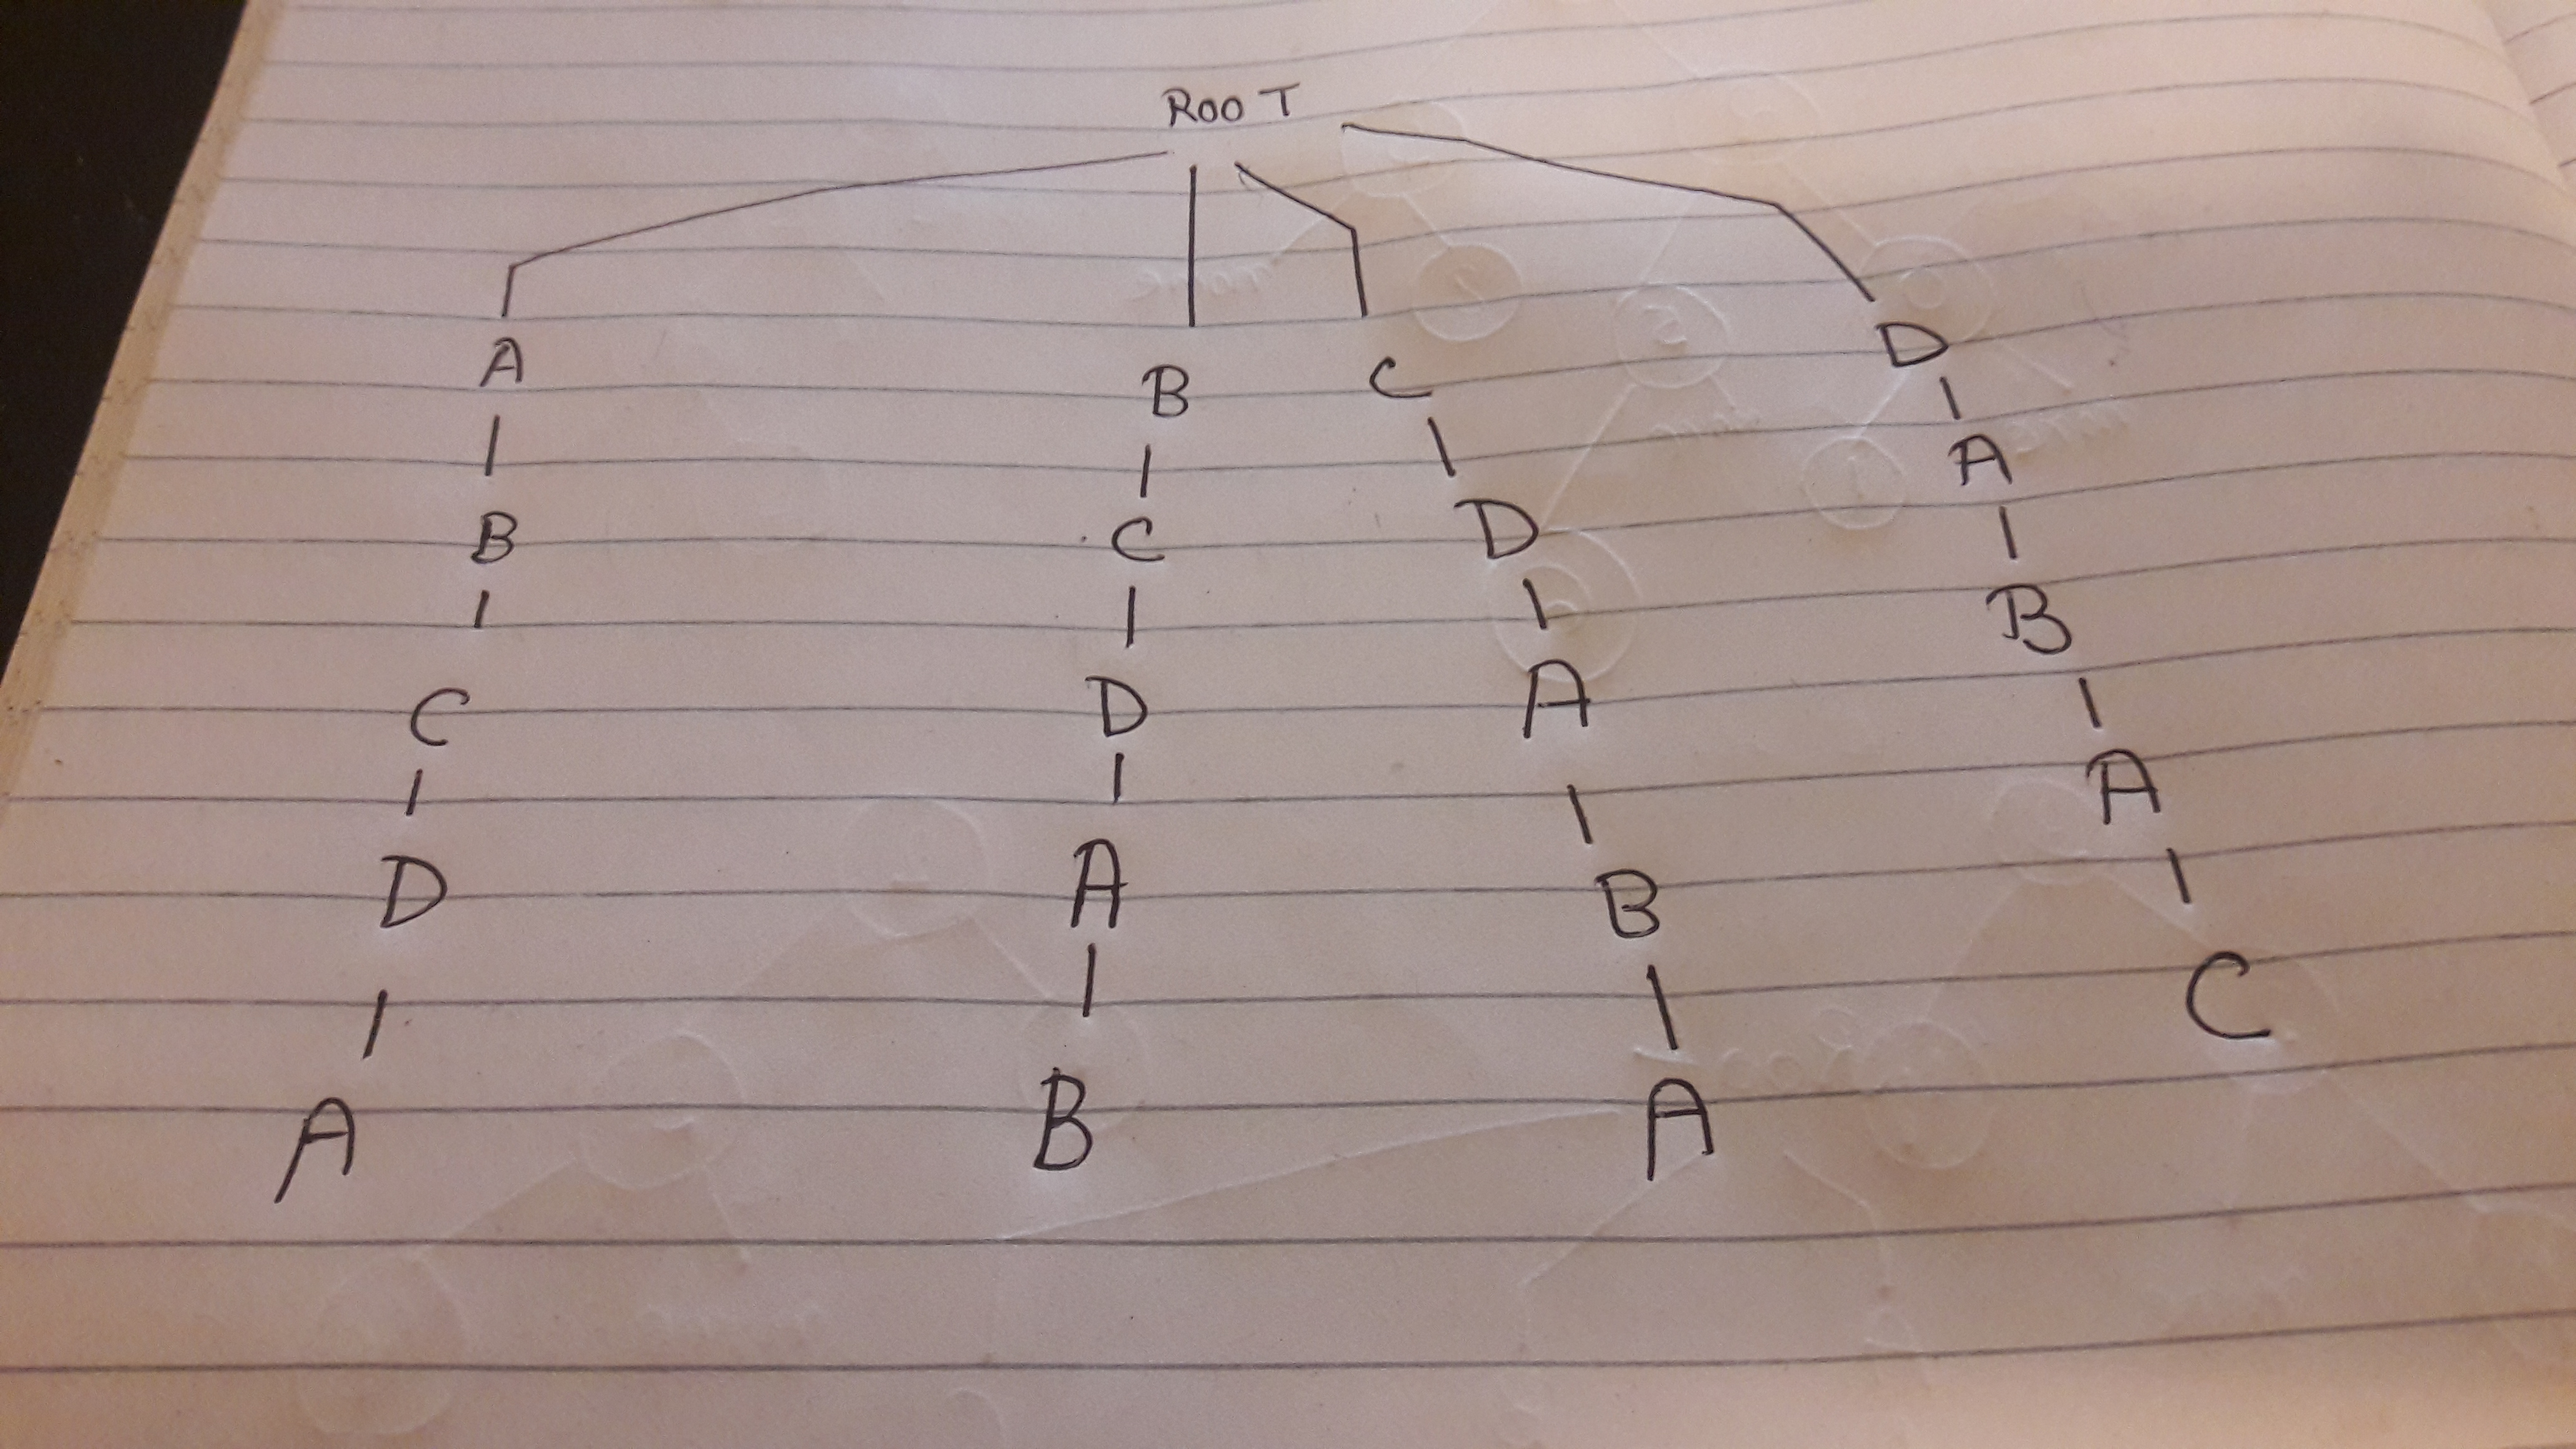
\includegraphics[scale=0.05]{16.jpg}


Midway through adding strings:






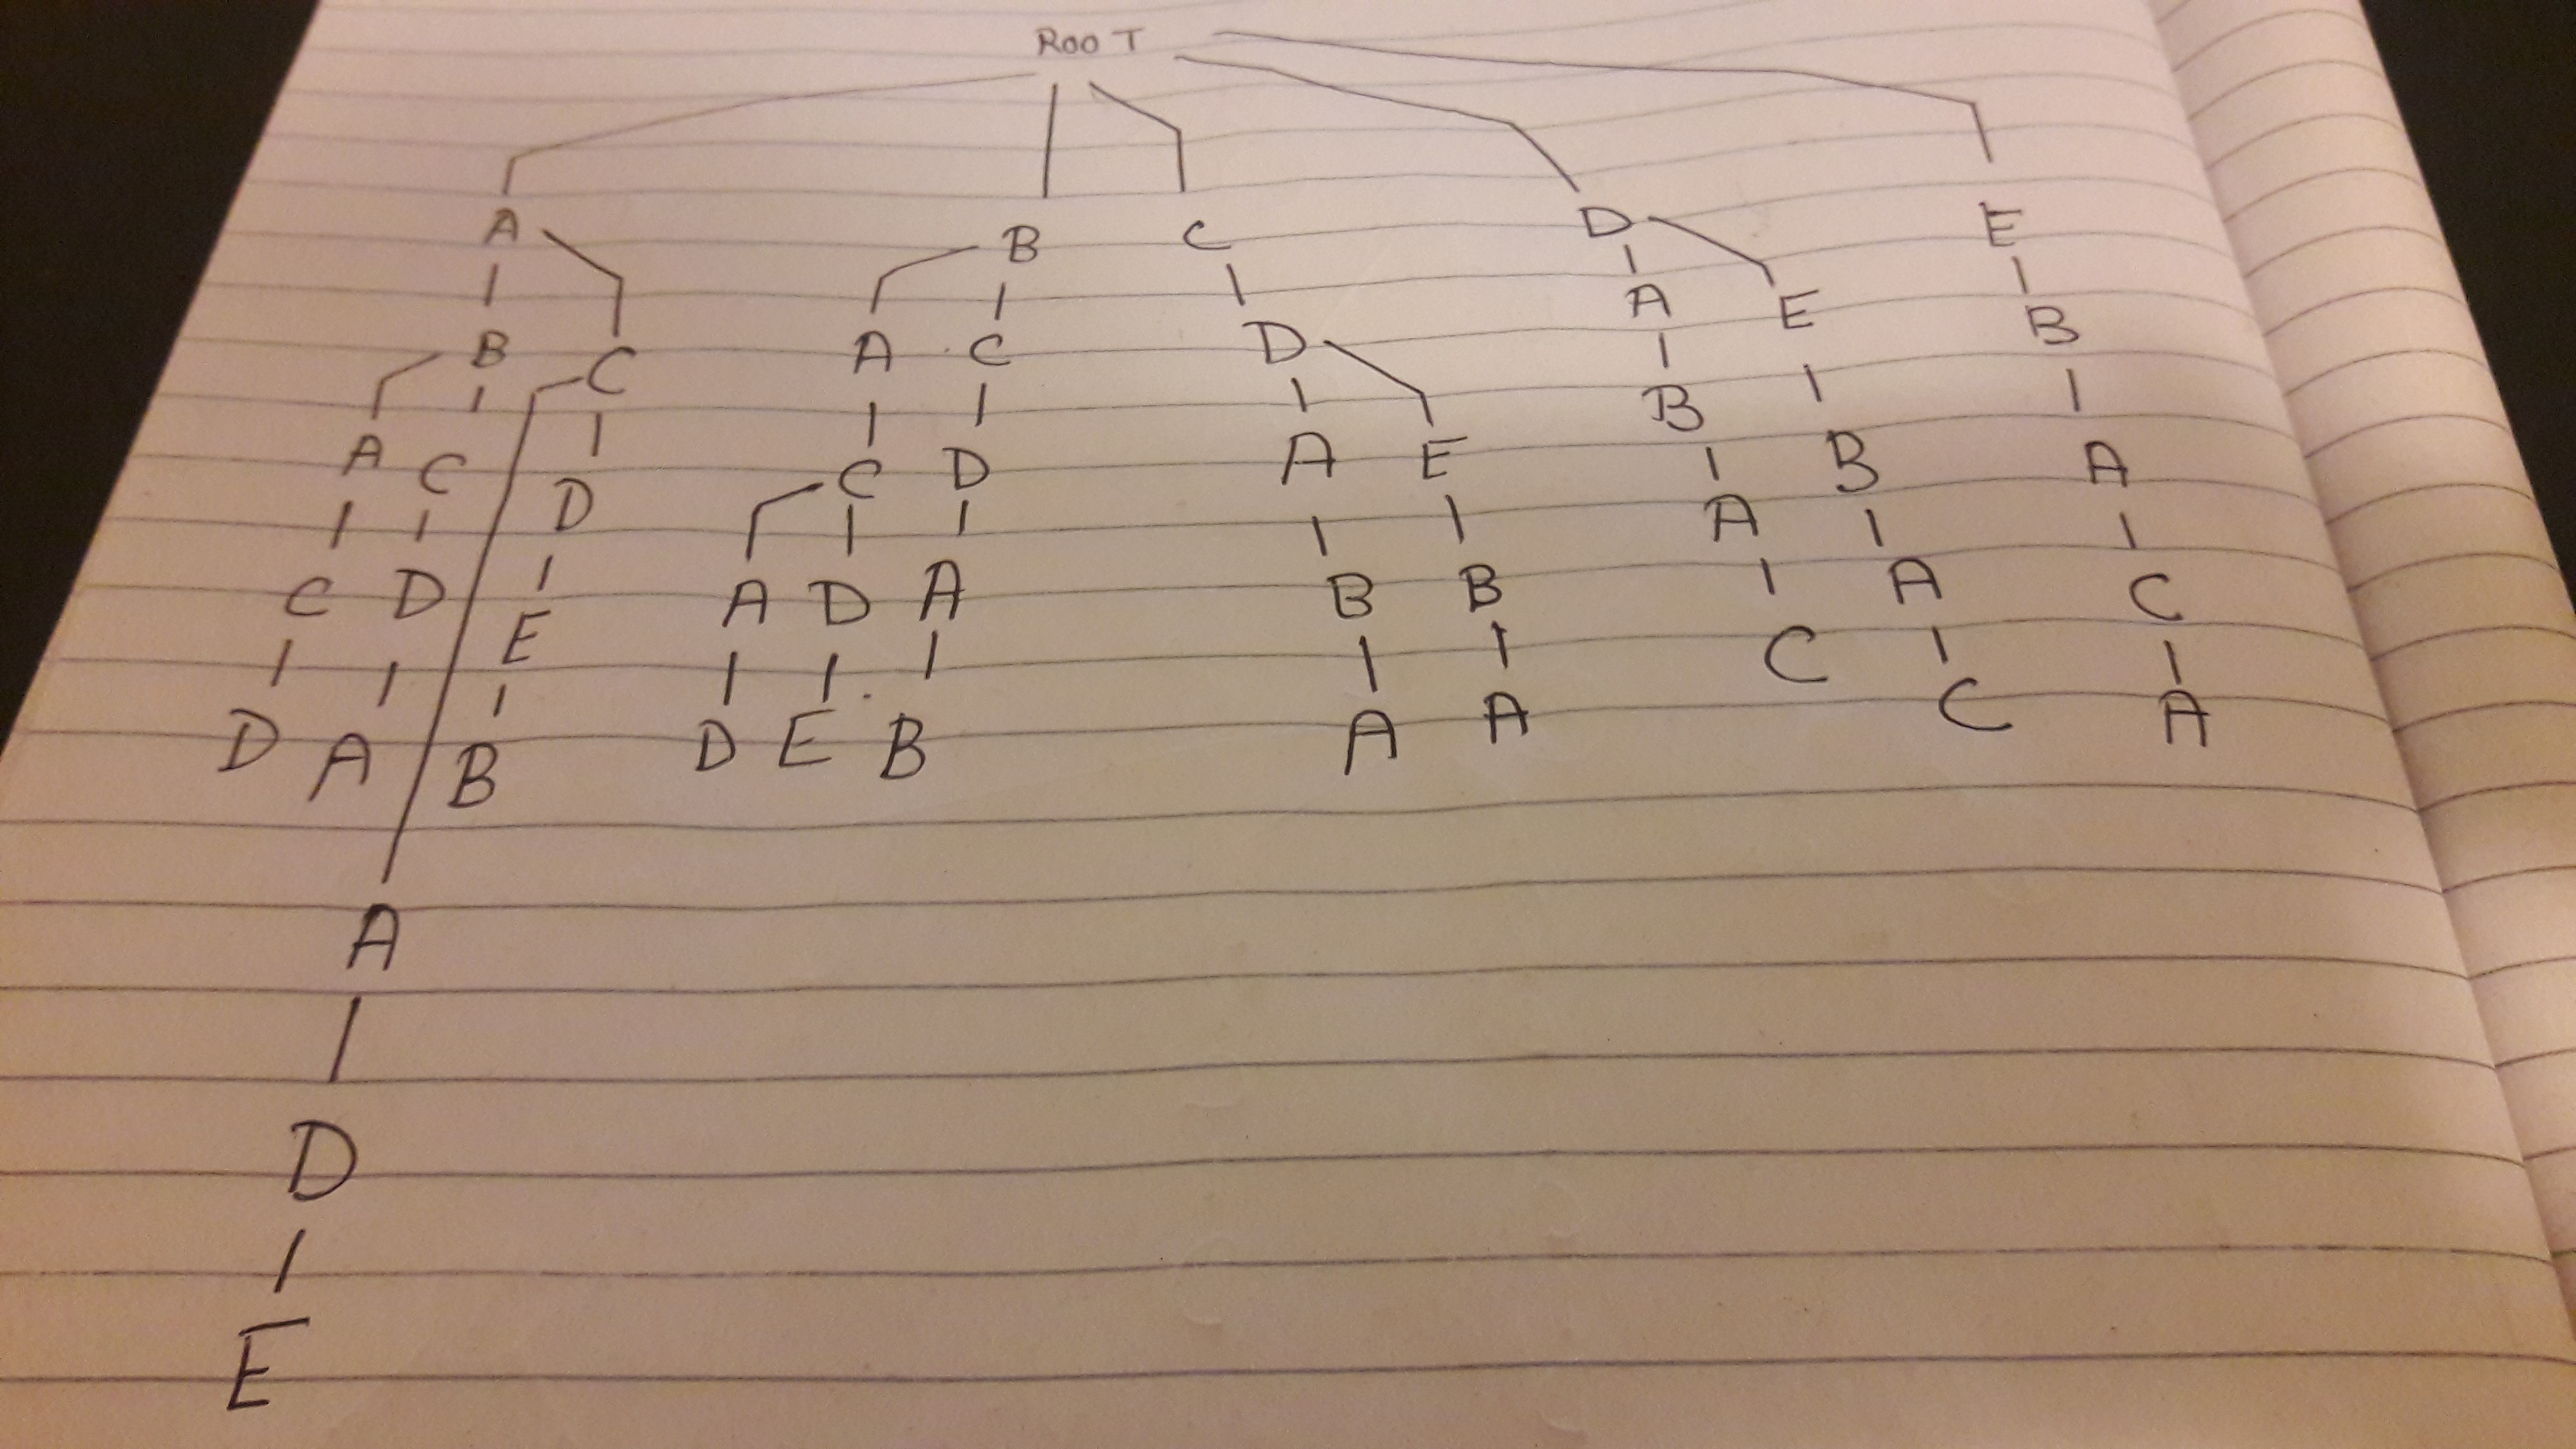
\includegraphics[scale=0.1]{17.jpg}



Final trie:



\includegraphics[scale=0.1]{18.jpg}





\section*{Question 4}

Step 1:



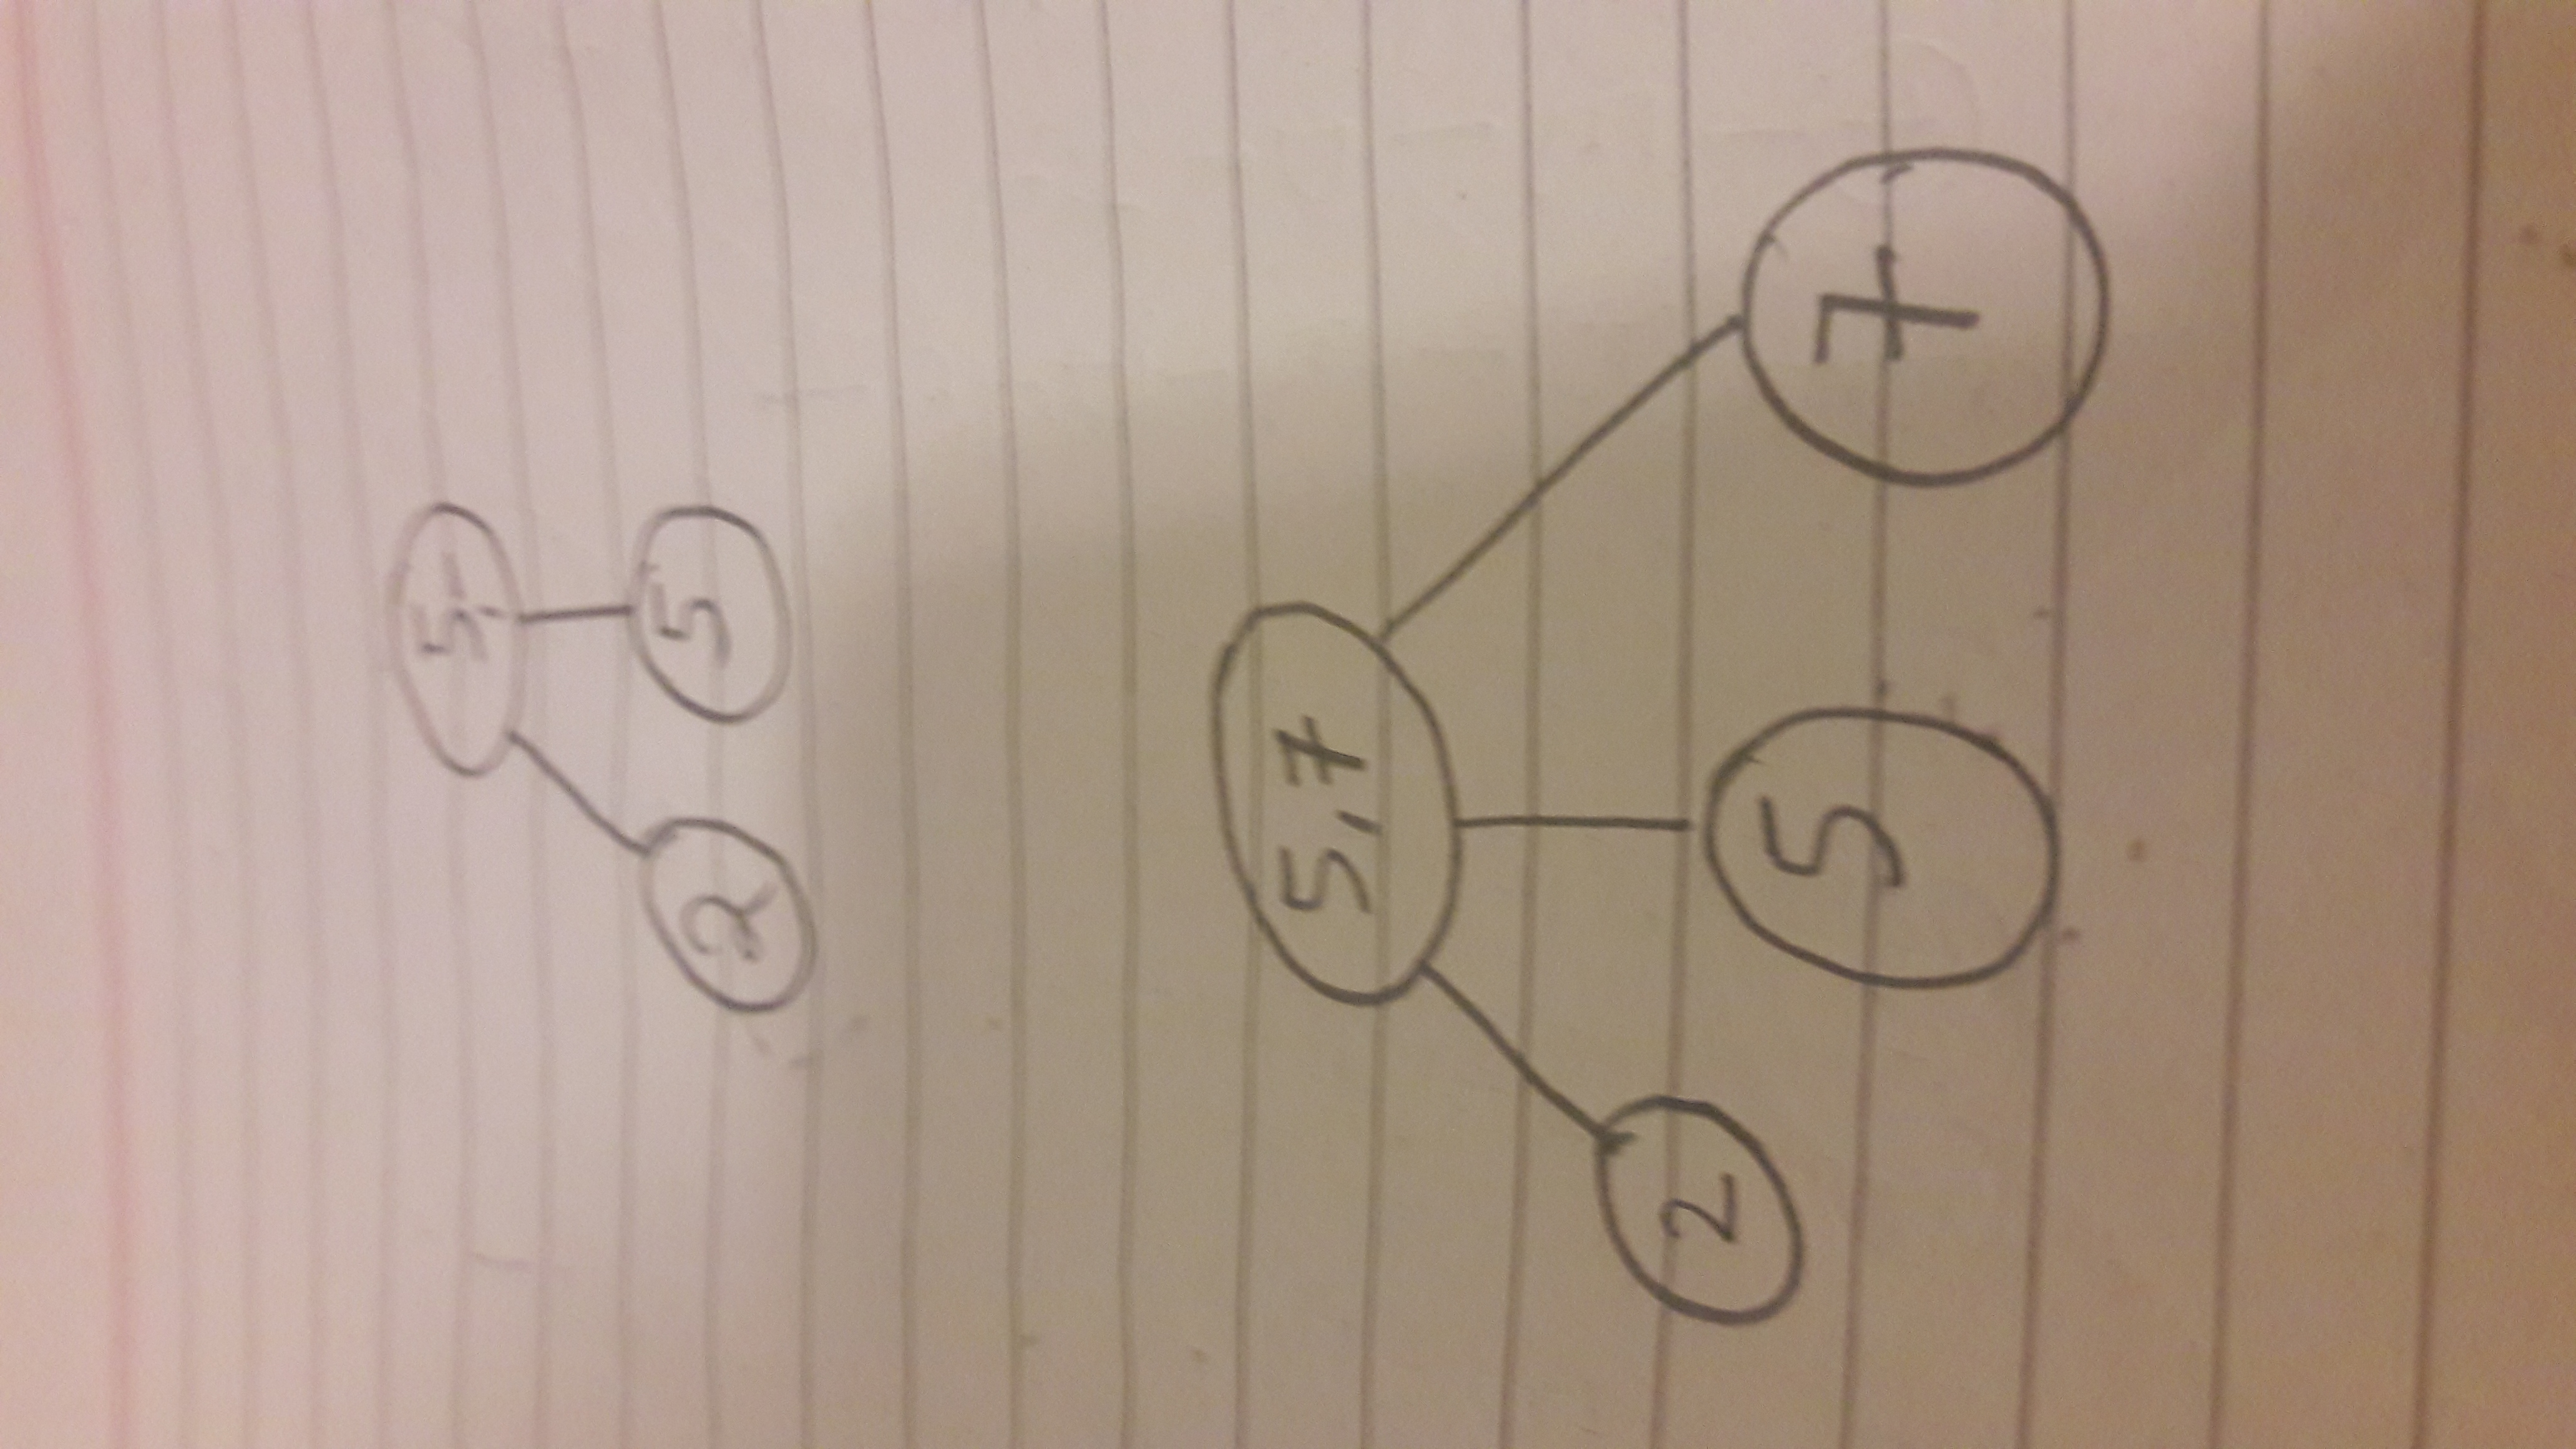
\includegraphics[scale=0.05]{19.jpg}



Step 2:



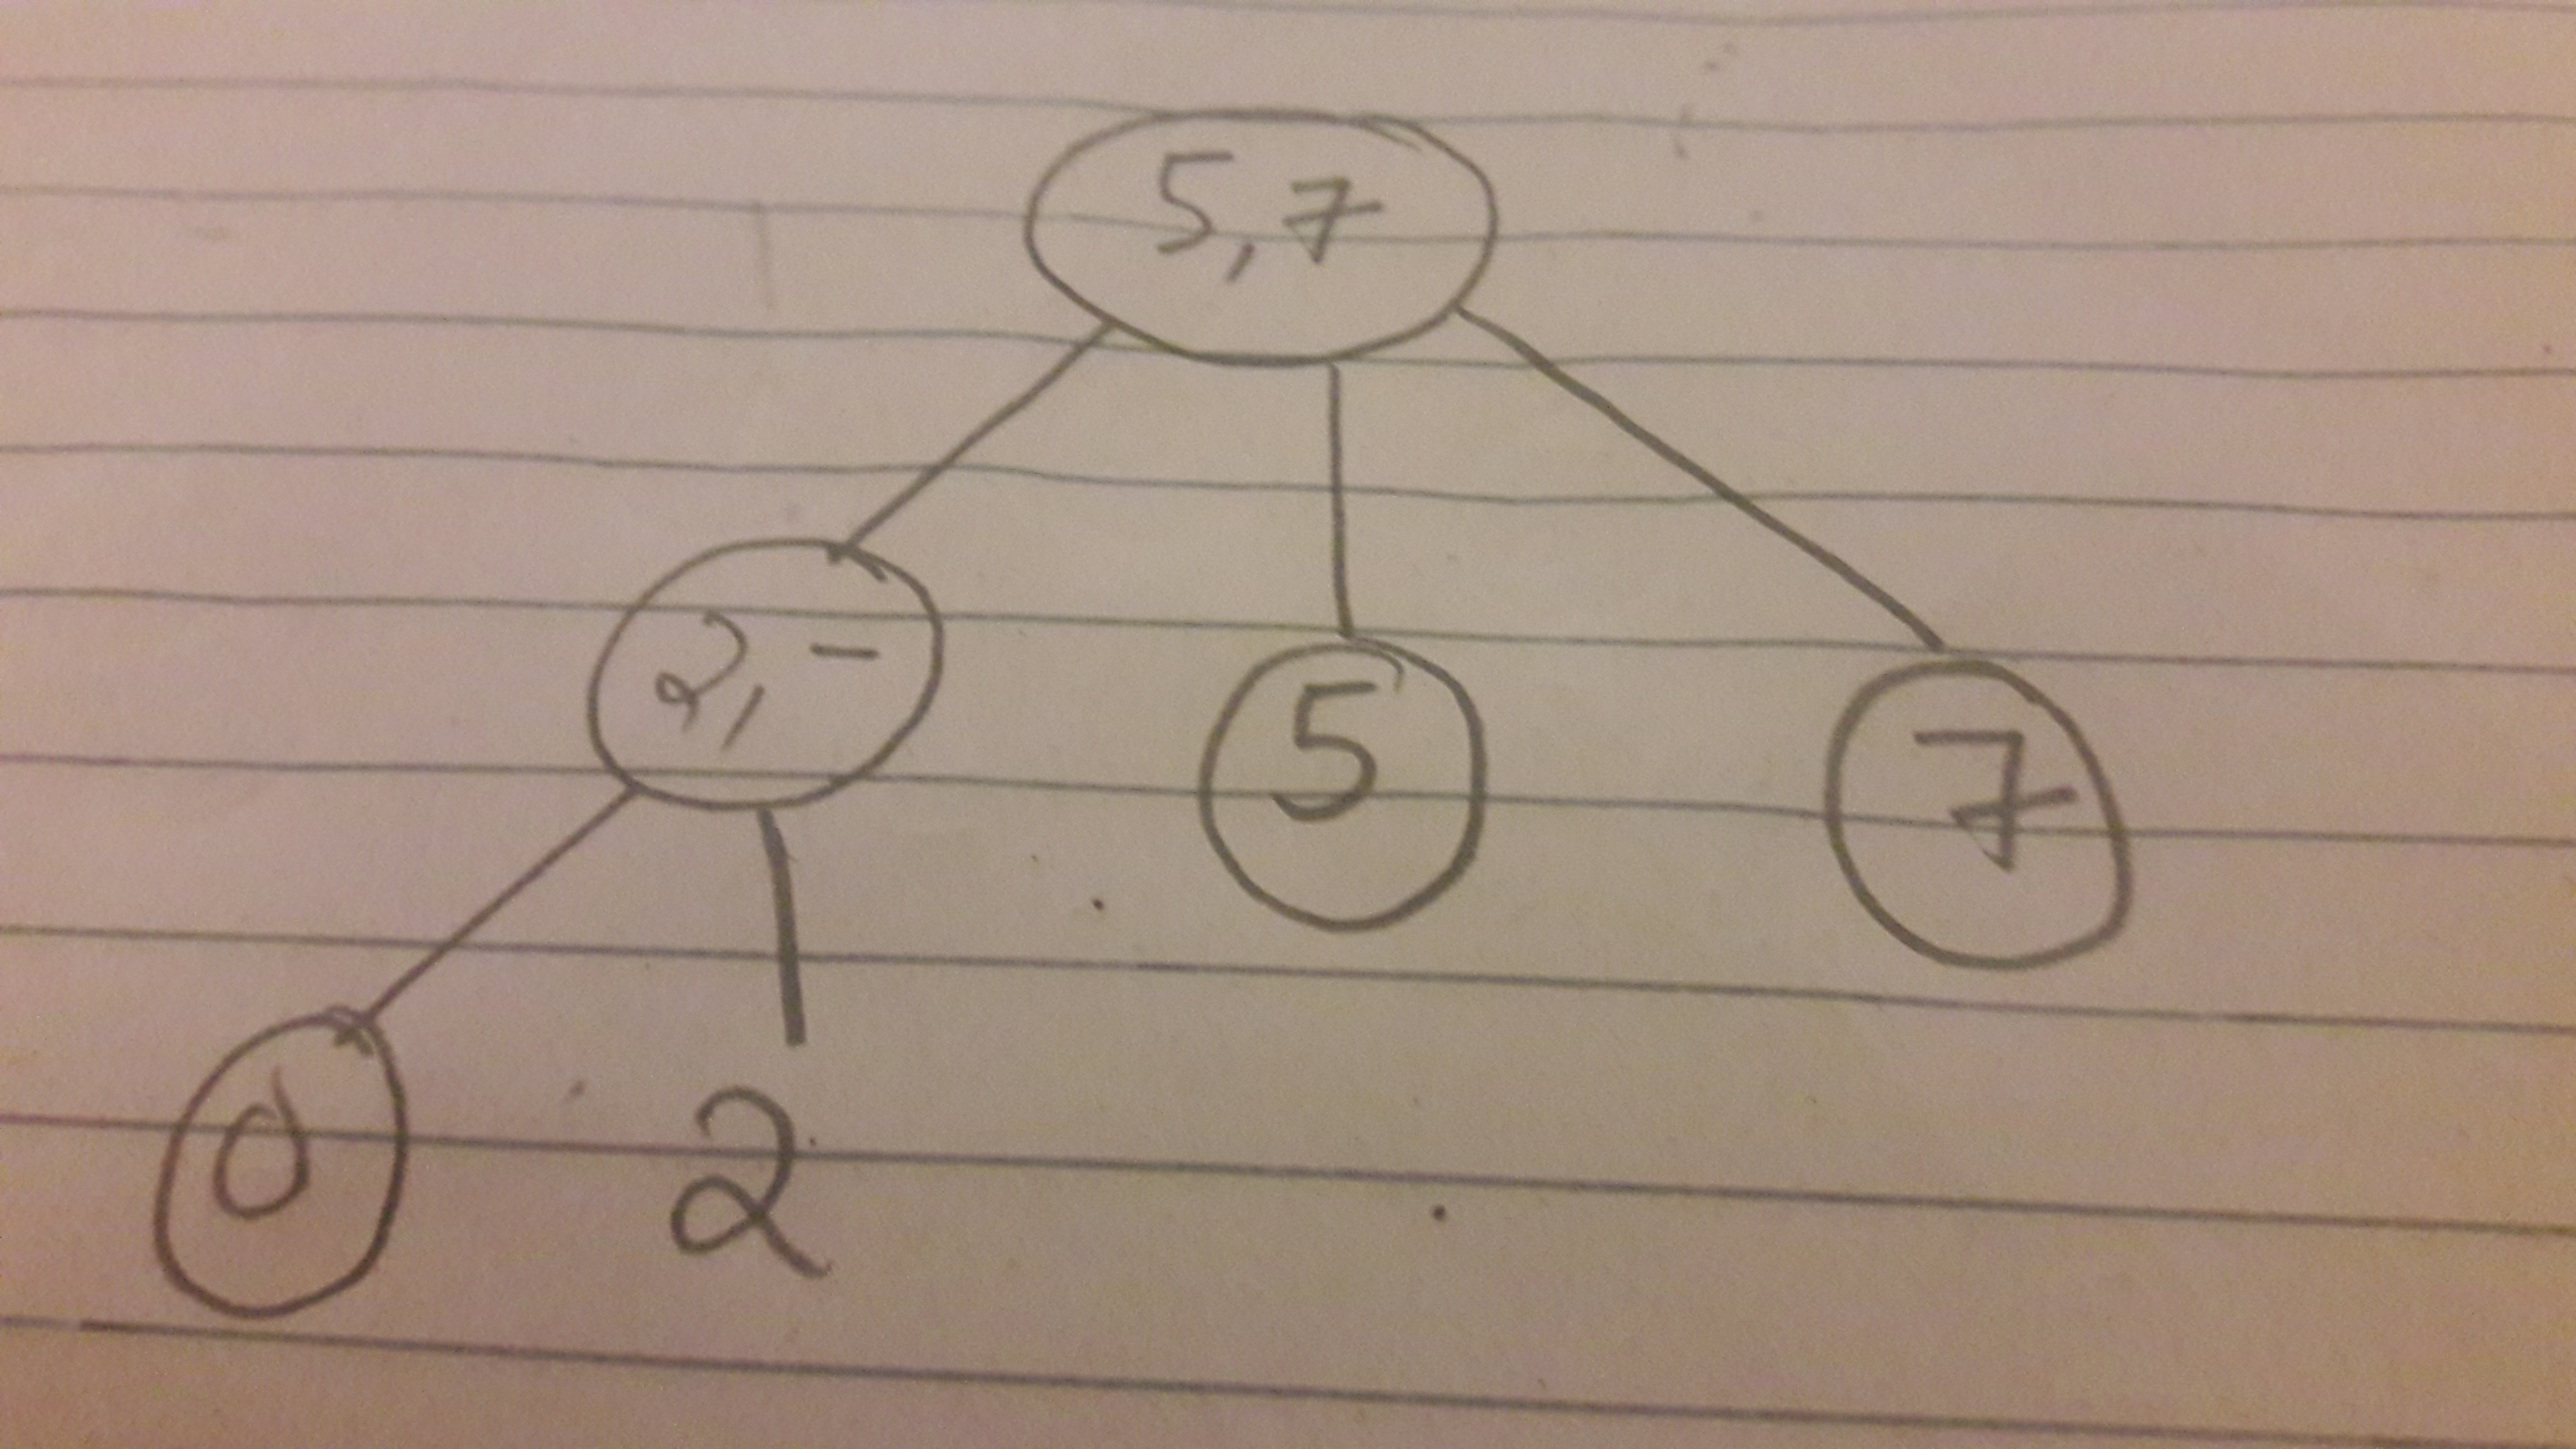
\includegraphics[scale=0.1]{20.jpg}



Step 3:



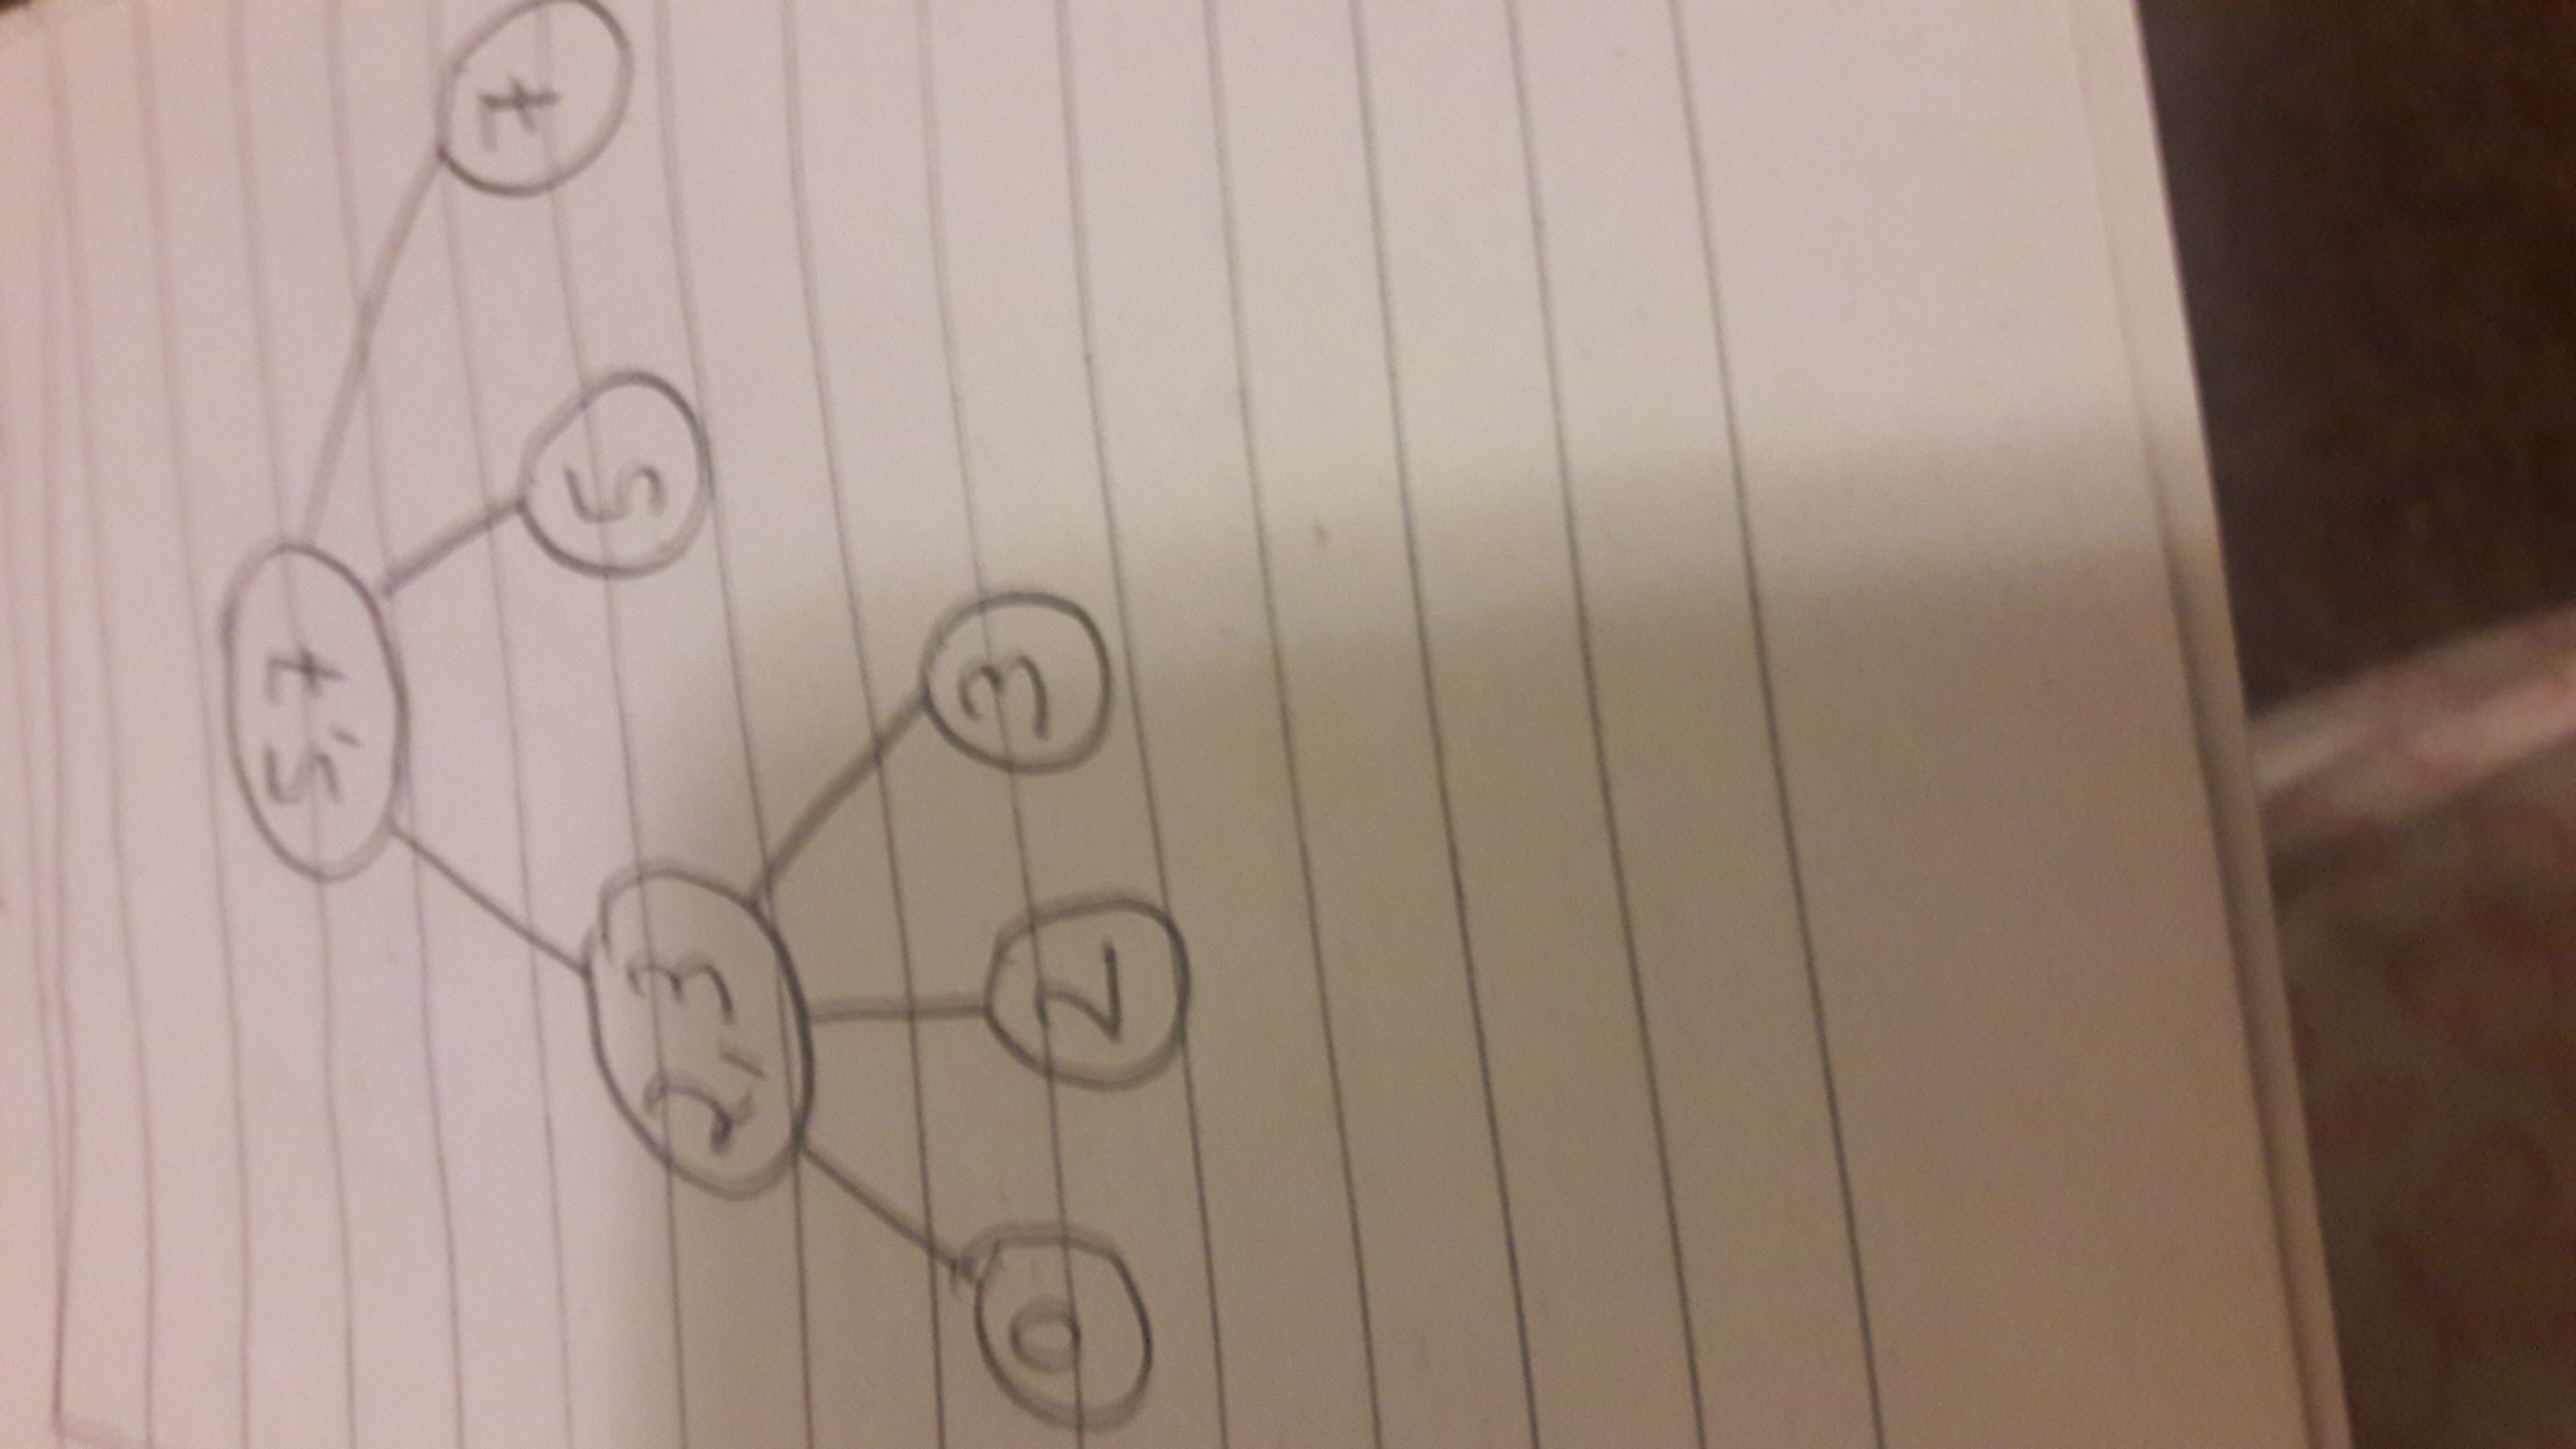
\includegraphics[scale=0.1]{21.jpg}



Step 4:



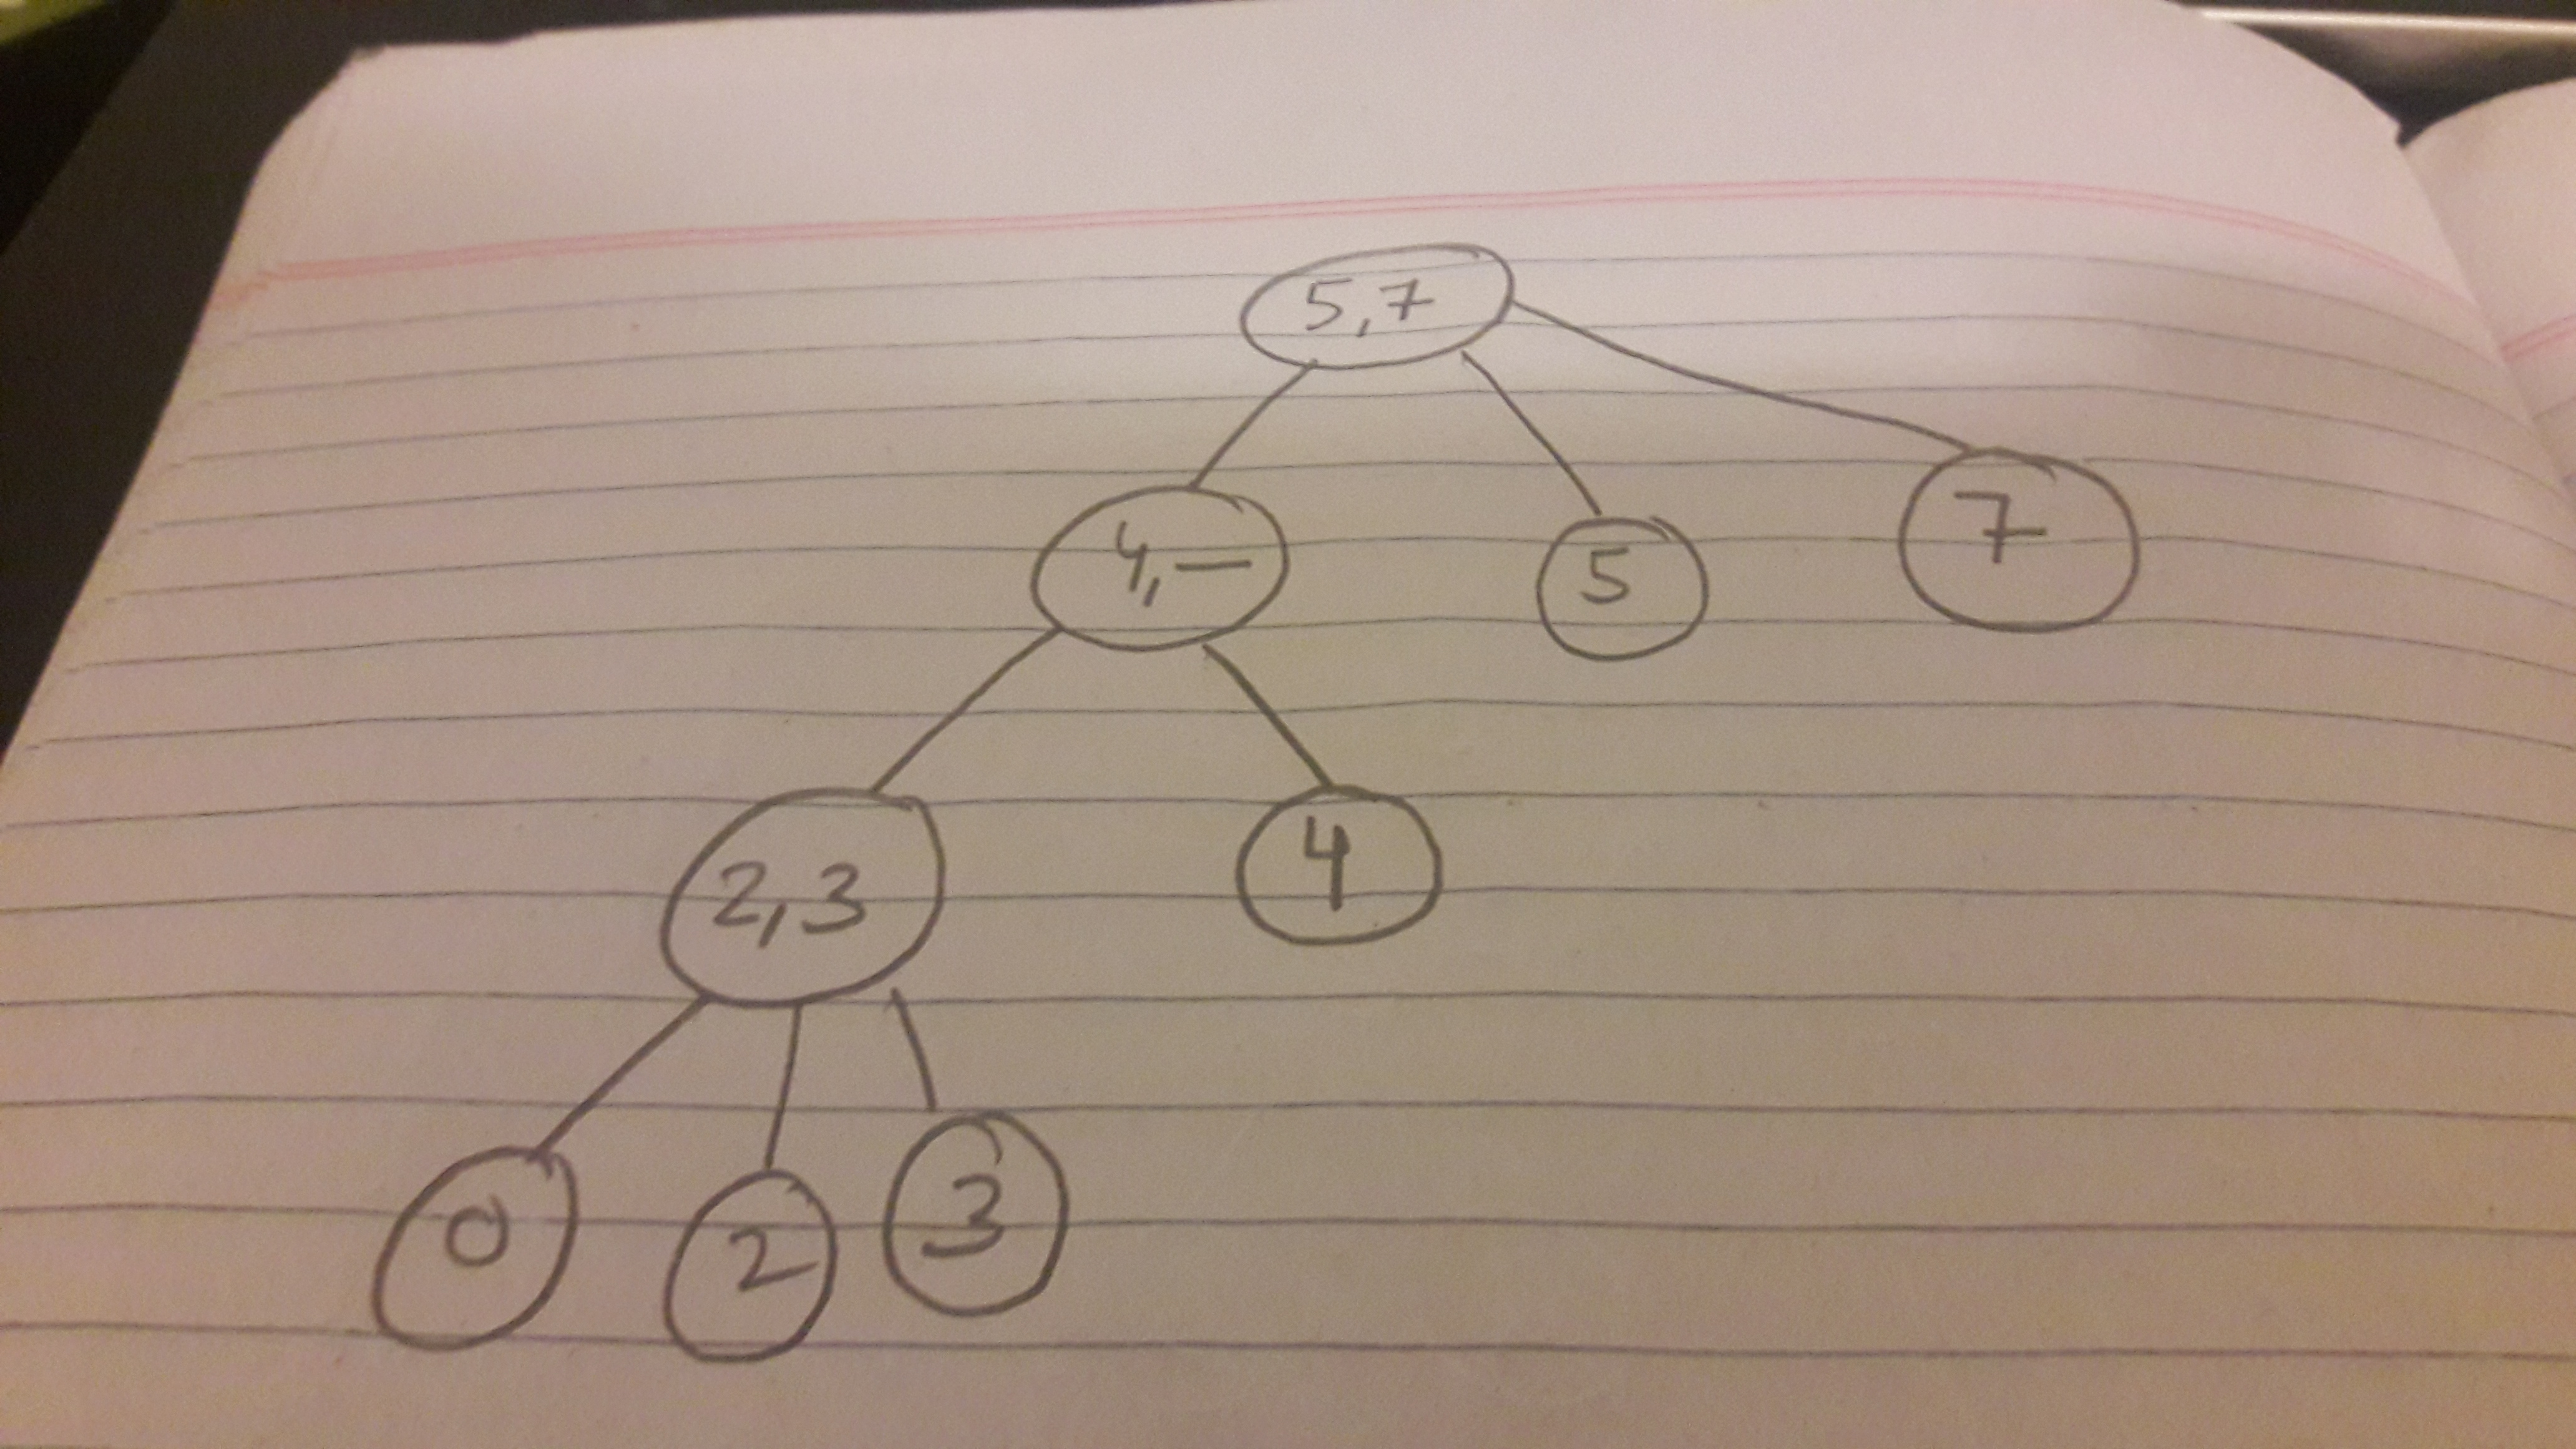
\includegraphics[scale=0.1]{22.jpg}




Step 5:




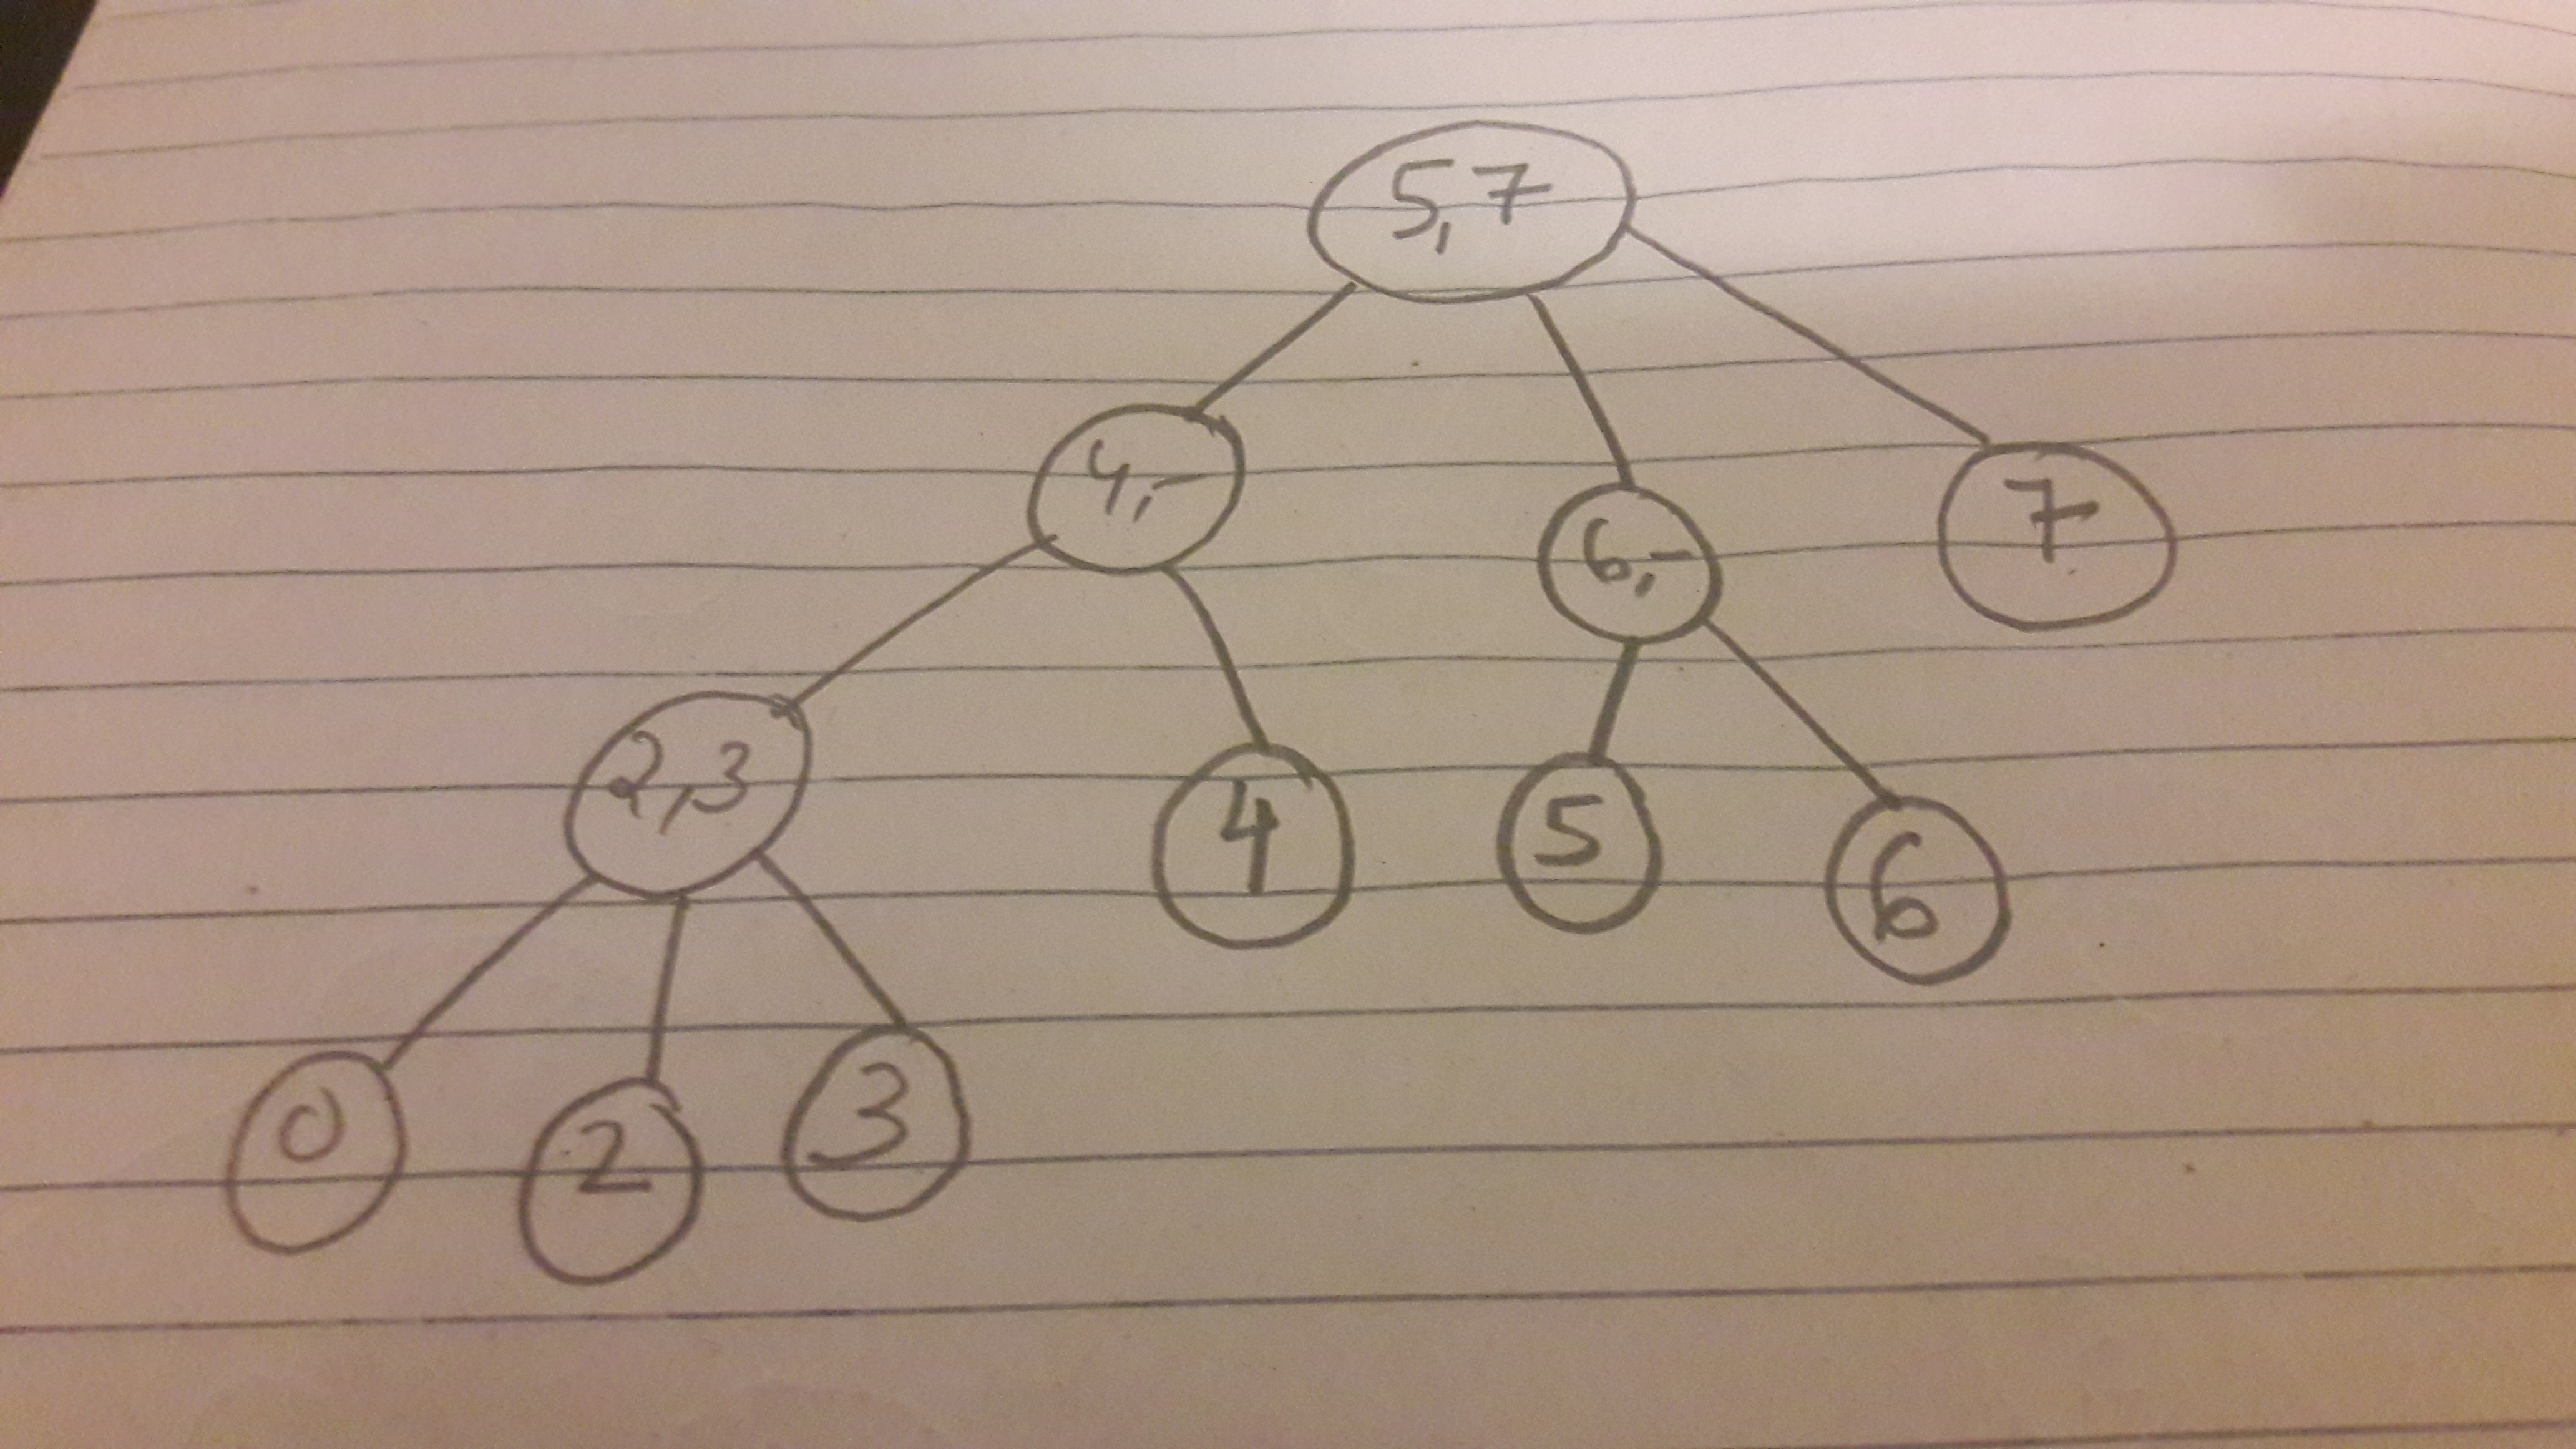
\includegraphics[scale=0.1]{23.jpg}



Final 2-3 tree:



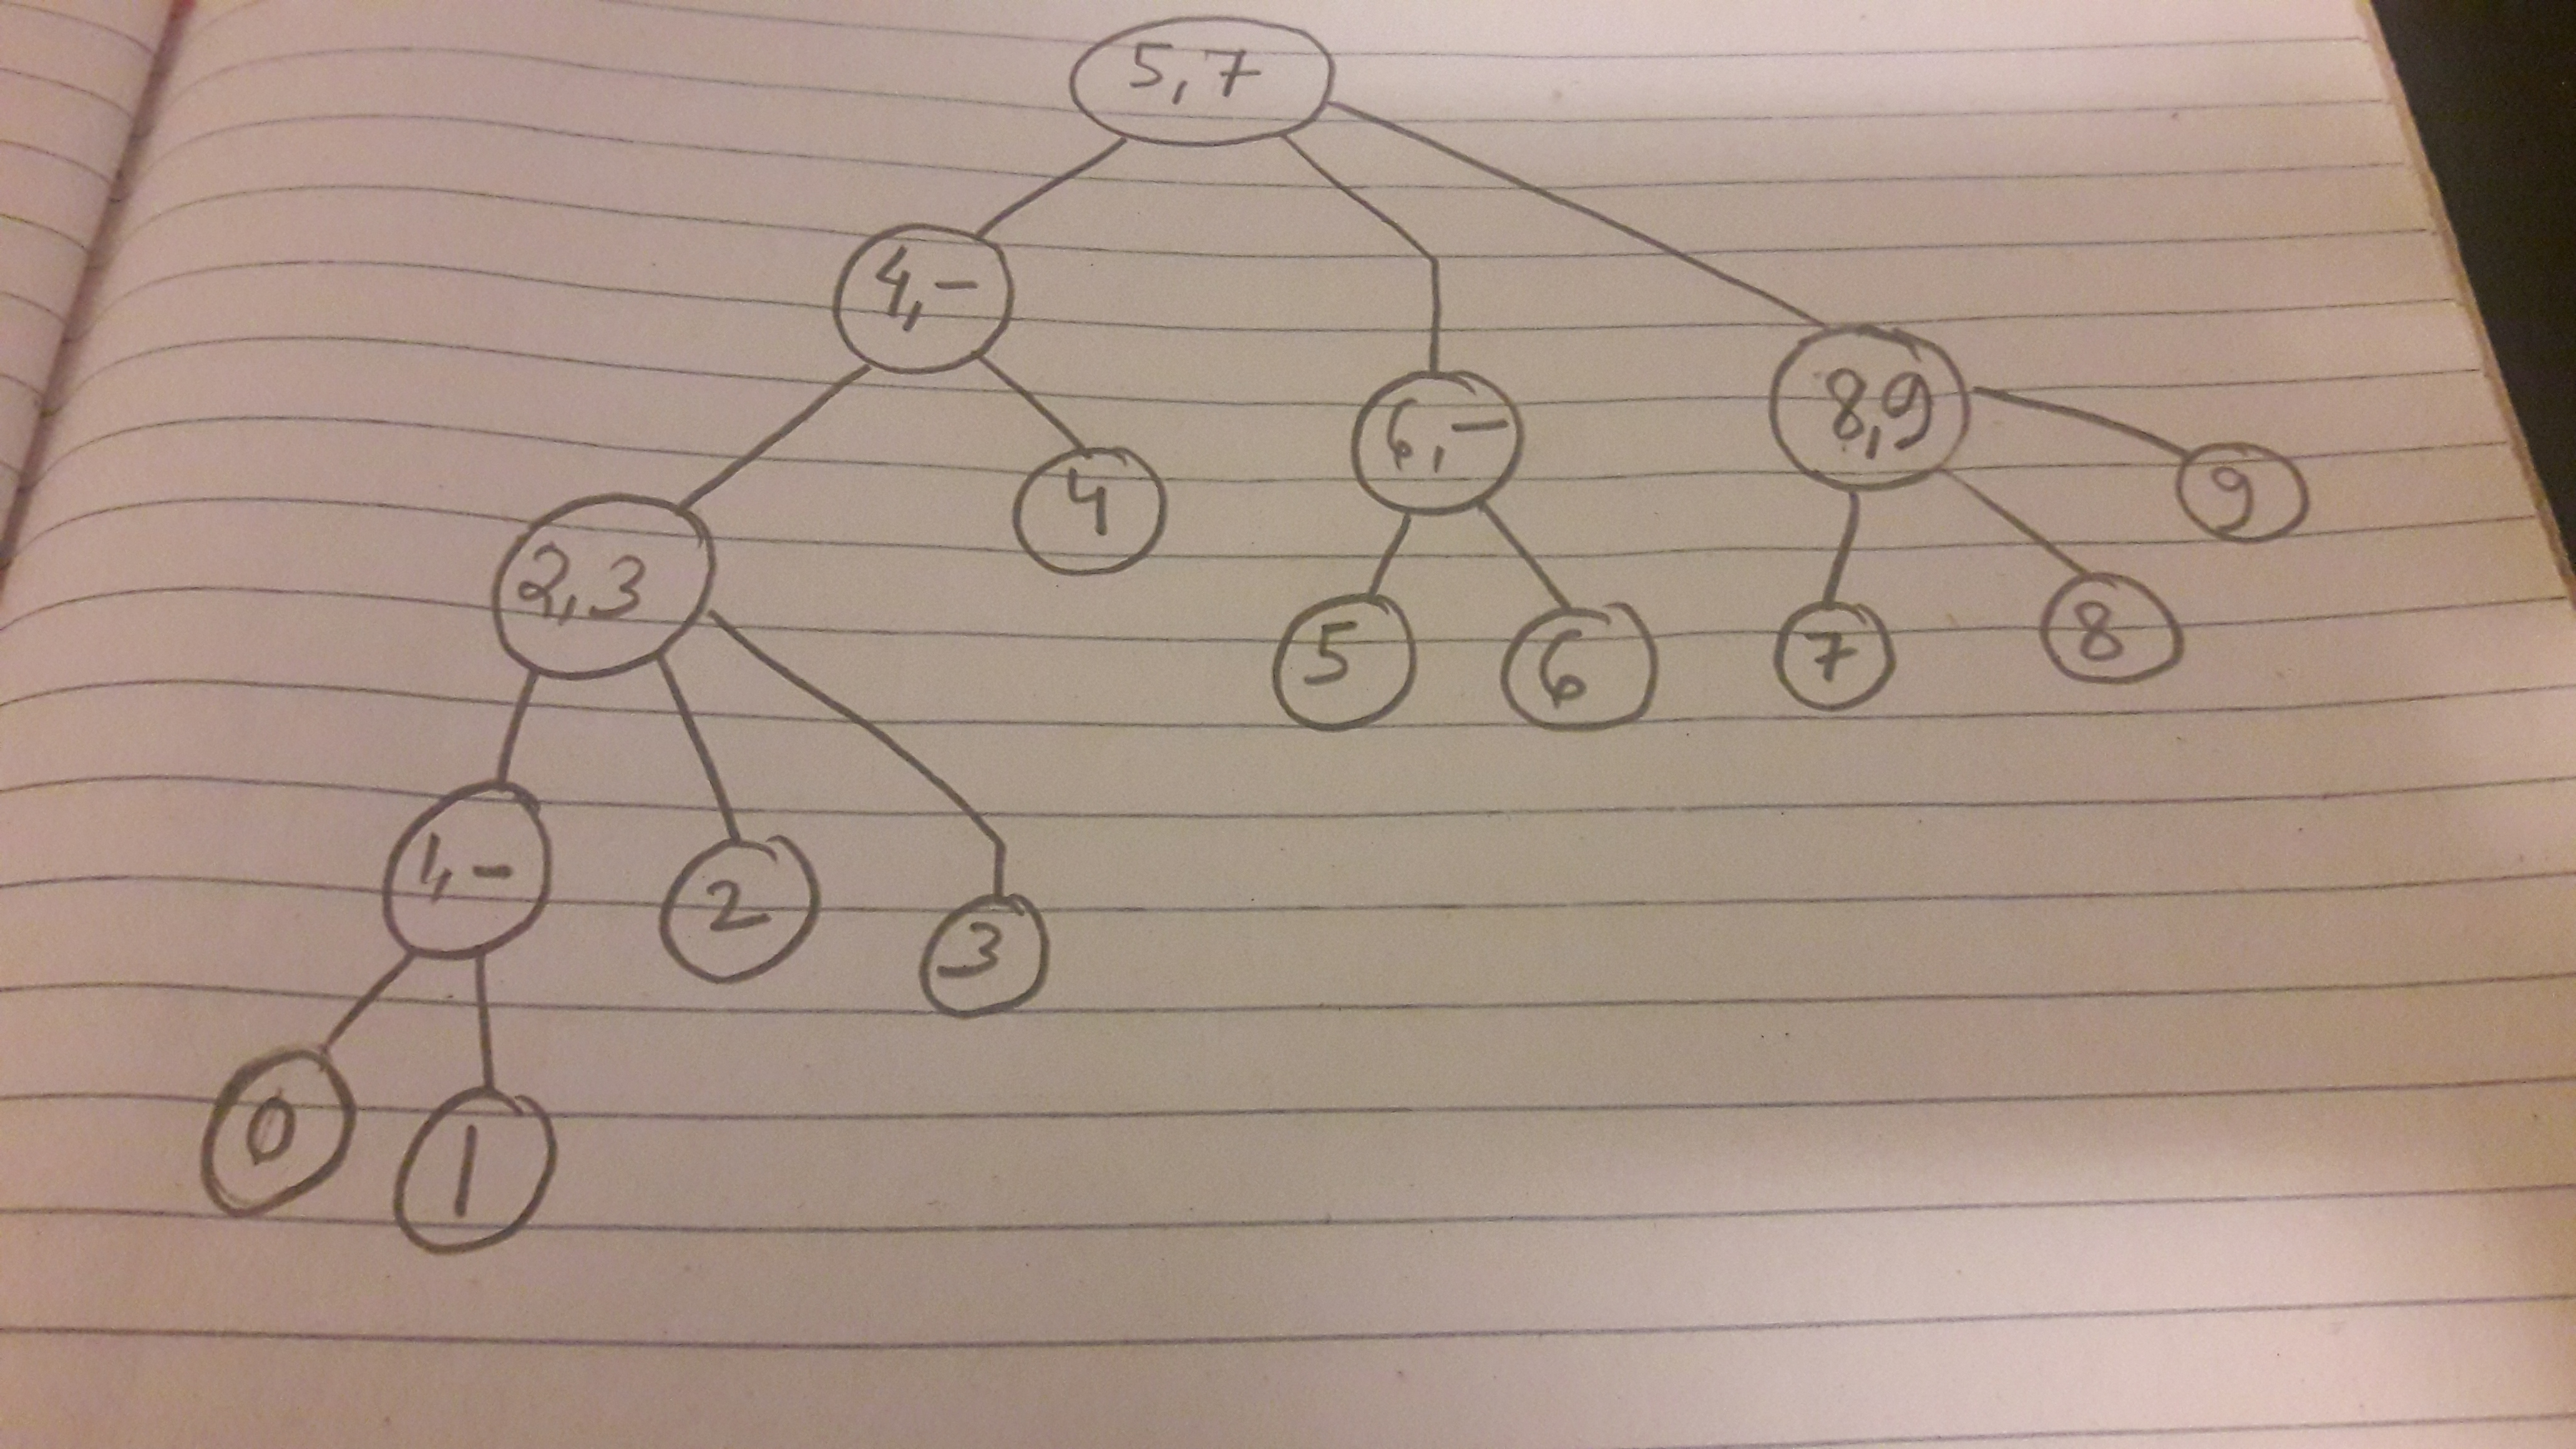
\includegraphics[scale=0.1]{24.jpg}



\end{document}

